%%%%%%%%%%%%%%%%%%%%%%%%%%%%%%%%%%%%%%%%%%%%%%%%%%%%%%%%%%%%%%%%%%%%%%%%%%%%%%%%%%%%%%%%%%
%                                     SETTINGS                                           %
%%%%%%%%%%%%%%%%%%%%%%%%%%%%%%%%%%%%%%%%%%%%%%%%%%%%%%%%%%%%%%%%%%%%%%%%%%%%%%%%%%%%%%%%%%
\documentclass[aspectratio=169, t]{beamer}

\usepackage{amsmath,amssymb}
\usepackage{graphics}
\usepackage{graphicx}
\usepackage{subcaption}
\usepackage{standalone}
\usepackage[makeroom]{cancel}
\usepackage{appendixnumberbeamer}
\usepackage{hyperref}
\usepackage{booktabs}
\usepackage{tikz}
\usepackage{xcolor}
\usepackage{units}

\graphicspath{{../../../analysis/}{../../../descriptive/}}

\usetheme{default}

\setbeamertemplate{itemize items}[circle]
\setbeamertemplate{footline}[frame number]
\setbeamertemplate{navigation symbols}{}

\usepackage[backend = bibtex,
            style = authoryear,
            maxnames = 5,
            maxcitenames = 3,
            doi = false,
            eprint = false]{biblatex}
\addbibresource{../../biblio.bib}

\definecolor{BgBlue}{rgb}{0.2,0.2,0.7}

\AtBeginSection[]{
    \begin{frame}
        \vfill
        \centering
        \begin{beamercolorbox}[sep=8pt,center,shadow=false,rounded=true]{title}
            \usebeamerfont{title}\insertsectionhead\par%
        \end{beamercolorbox}
        \vfill
    \end{frame}
}

\newtheorem{assu}{Assumption}
\newtheorem{prop}{Proposition}

\newcommand{\Z}{\mathcal{Z}}
\newcommand{\MW}{\underline{W}}
\newcommand{\mw}{\underline{w}}
\newcommand{\wkp}{\text{wkp}}
\newcommand{\res}{\text{res}}
\newcommand{\pre}{\text{Pre}}
\newcommand{\post}{\text{Post}}

%%%%%%%%%%%%%%%%%%%%%%%%%%%%%%%%%%%%%%%%%%%%%%%%%%%%%%%%%%%%%%%%%%%%%%%%%%%%%%%%%%%%%%%%%%
%                                     TITLE                                              %
%%%%%%%%%%%%%%%%%%%%%%%%%%%%%%%%%%%%%%%%%%%%%%%%%%%%%%%%%%%%%%%%%%%%%%%%%%%%%%%%%%%%%%%%%%
\title{Minimum Wage as a Place-Based Policy:}
\subtitle{Evidence from US Housing Rental Markets}
\date{\today}
%\date{}
\author{Diego Gentile Passaro \and Santiago Hermo \and Gabriele Borg}
\institute{Brown University $ \quad\quad\quad\quad $ Brown University $ \quad\quad\quad\quad$  AWS}
% \titlegraphic{\hfill\includegraphics[height=1.5cm]{logo.pdf}}

%%%%%%%%%%%%%%%%%%%%%%%%%%%%%%%%%%%%%%%%%%%%%%%%%%%%%%%%%%%%%%%%%%%%%%%%%%%%%%%%%%%%%%%%%%
%                                         BODY                                           %
%%%%%%%%%%%%%%%%%%%%%%%%%%%%%%%%%%%%%%%%%%%%%%%%%%%%%%%%%%%%%%%%%%%%%%%%%%%%%%%%%%%%%%%%%%
\begin{document}
\maketitle


%%% Introduction %%%

\begin{frame}
    \frametitle{Motivation}
    
    Minimum wage policies attempt to improve the livelihoods of low-wage workers.
    \begin{itemize}
        \item Increase wages with small effects on employment
        {\small \color{gray} \parencite[e.g.,][]{CegnizEtAl2019}}
        \item Decrease inequality {\small \color{gray} \parencite{AutorEtAl2016}}
        and poverty {\small \color{gray} \parencite{Dube2019Income}}
    \end{itemize}

    \vspace{2mm}
    \pause
    However, %as low-wage workers are more likely to rent houses, 
    a significant pass-through of MWs to rents may undermine the objectives of the policy.
    
    %% Plot showing probability of renting by income

\end{frame}

\begin{frame}
    \frametitle{Motivation}
    
    Research on minimum wage (MW) has mostly focused on labor market outcomes.
    % States: only workplace MW matters
    
    \begin{itemize}
        \item But MW policies are \textit{place-based} $\Rightarrow$ Housing market
    \end{itemize}

    \pause
    \vspace{3mm}
    Large variation of MW levels in the US even within metropolitan areas.
    
    \begin{itemize}
        \item Divergence between MW levels at workplace and residence
        \item Expect spatially heterogeneous effects
    \end{itemize}
\end{frame}

\begin{frame}
    \frametitle{This paper}
    
    What we do
    \begin{itemize}
        \vspace{.5mm} \item Accounting for spatial spillovers, estimate 
        elasticity of rents in the local housing market to
         {\color{blue} workplace MW} and {\color{red} residence MW} changes
        \vspace{.5mm} \item Estimate share of the extra dollar generated by
        MW increases pocketed by landlords in each local market
    \end{itemize}
    
    \vspace{3mm}
    \pause
    How we do it
    \begin{itemize}
        \vspace{.5mm} \item Propose a novel measure of exposure to MW changes 
        based on commuting shares
        \vspace{.5mm} \item Construct novel dataset of MW policies at ZIP code level
        \vspace{.5mm} \item Exploit high-frequency (month) high-resolution 
        (ZIP code) rents data from Zillow
        \vspace{.5mm} \item Leverage timing and spatial variation in MW changes 
        \textit{within} metropolitan areas
    \end{itemize}
\end{frame}

\begin{frame}
    \frametitle{An initial intuition}
    
    \vspace{3mm}
    
    Think of a metropolitan area and a MW increase in the business district (CBD). 
    
    \vspace{3mm}
    
    \textbf{Partial equilibrium: short term}
    \begin{itemize}
        \vspace{.5mm} \item Firms producing in the CBD will pay a higher wage. Income 
        redistribution from CBD consumers to low-income workers.
        \vspace{.5mm} \item Income changes are heterogeneous across space because people work 
        and reside in different locations.
        \vspace{.5mm} \item Housing is a normal good, so demand in some areas increases 
        and landlords charge a higher rent.
    \end{itemize}

    \pause
    \vspace{3mm}
    \textbf{General equilibrium: long term} (Not this paper!)
    \begin{itemize}
    \vspace{.5mm} \item People change residence and workplace locations (sorting).
    \vspace{.5mm} \item Developers build more houses (supply response).
\end{itemize}
\end{frame}

\begin{frame}
    \frametitle{A motivating example}
    \begin{columns}
        \begin{column}{0.44\textwidth}
            \vspace{-8mm}
            \begin{figure}
                \centering
                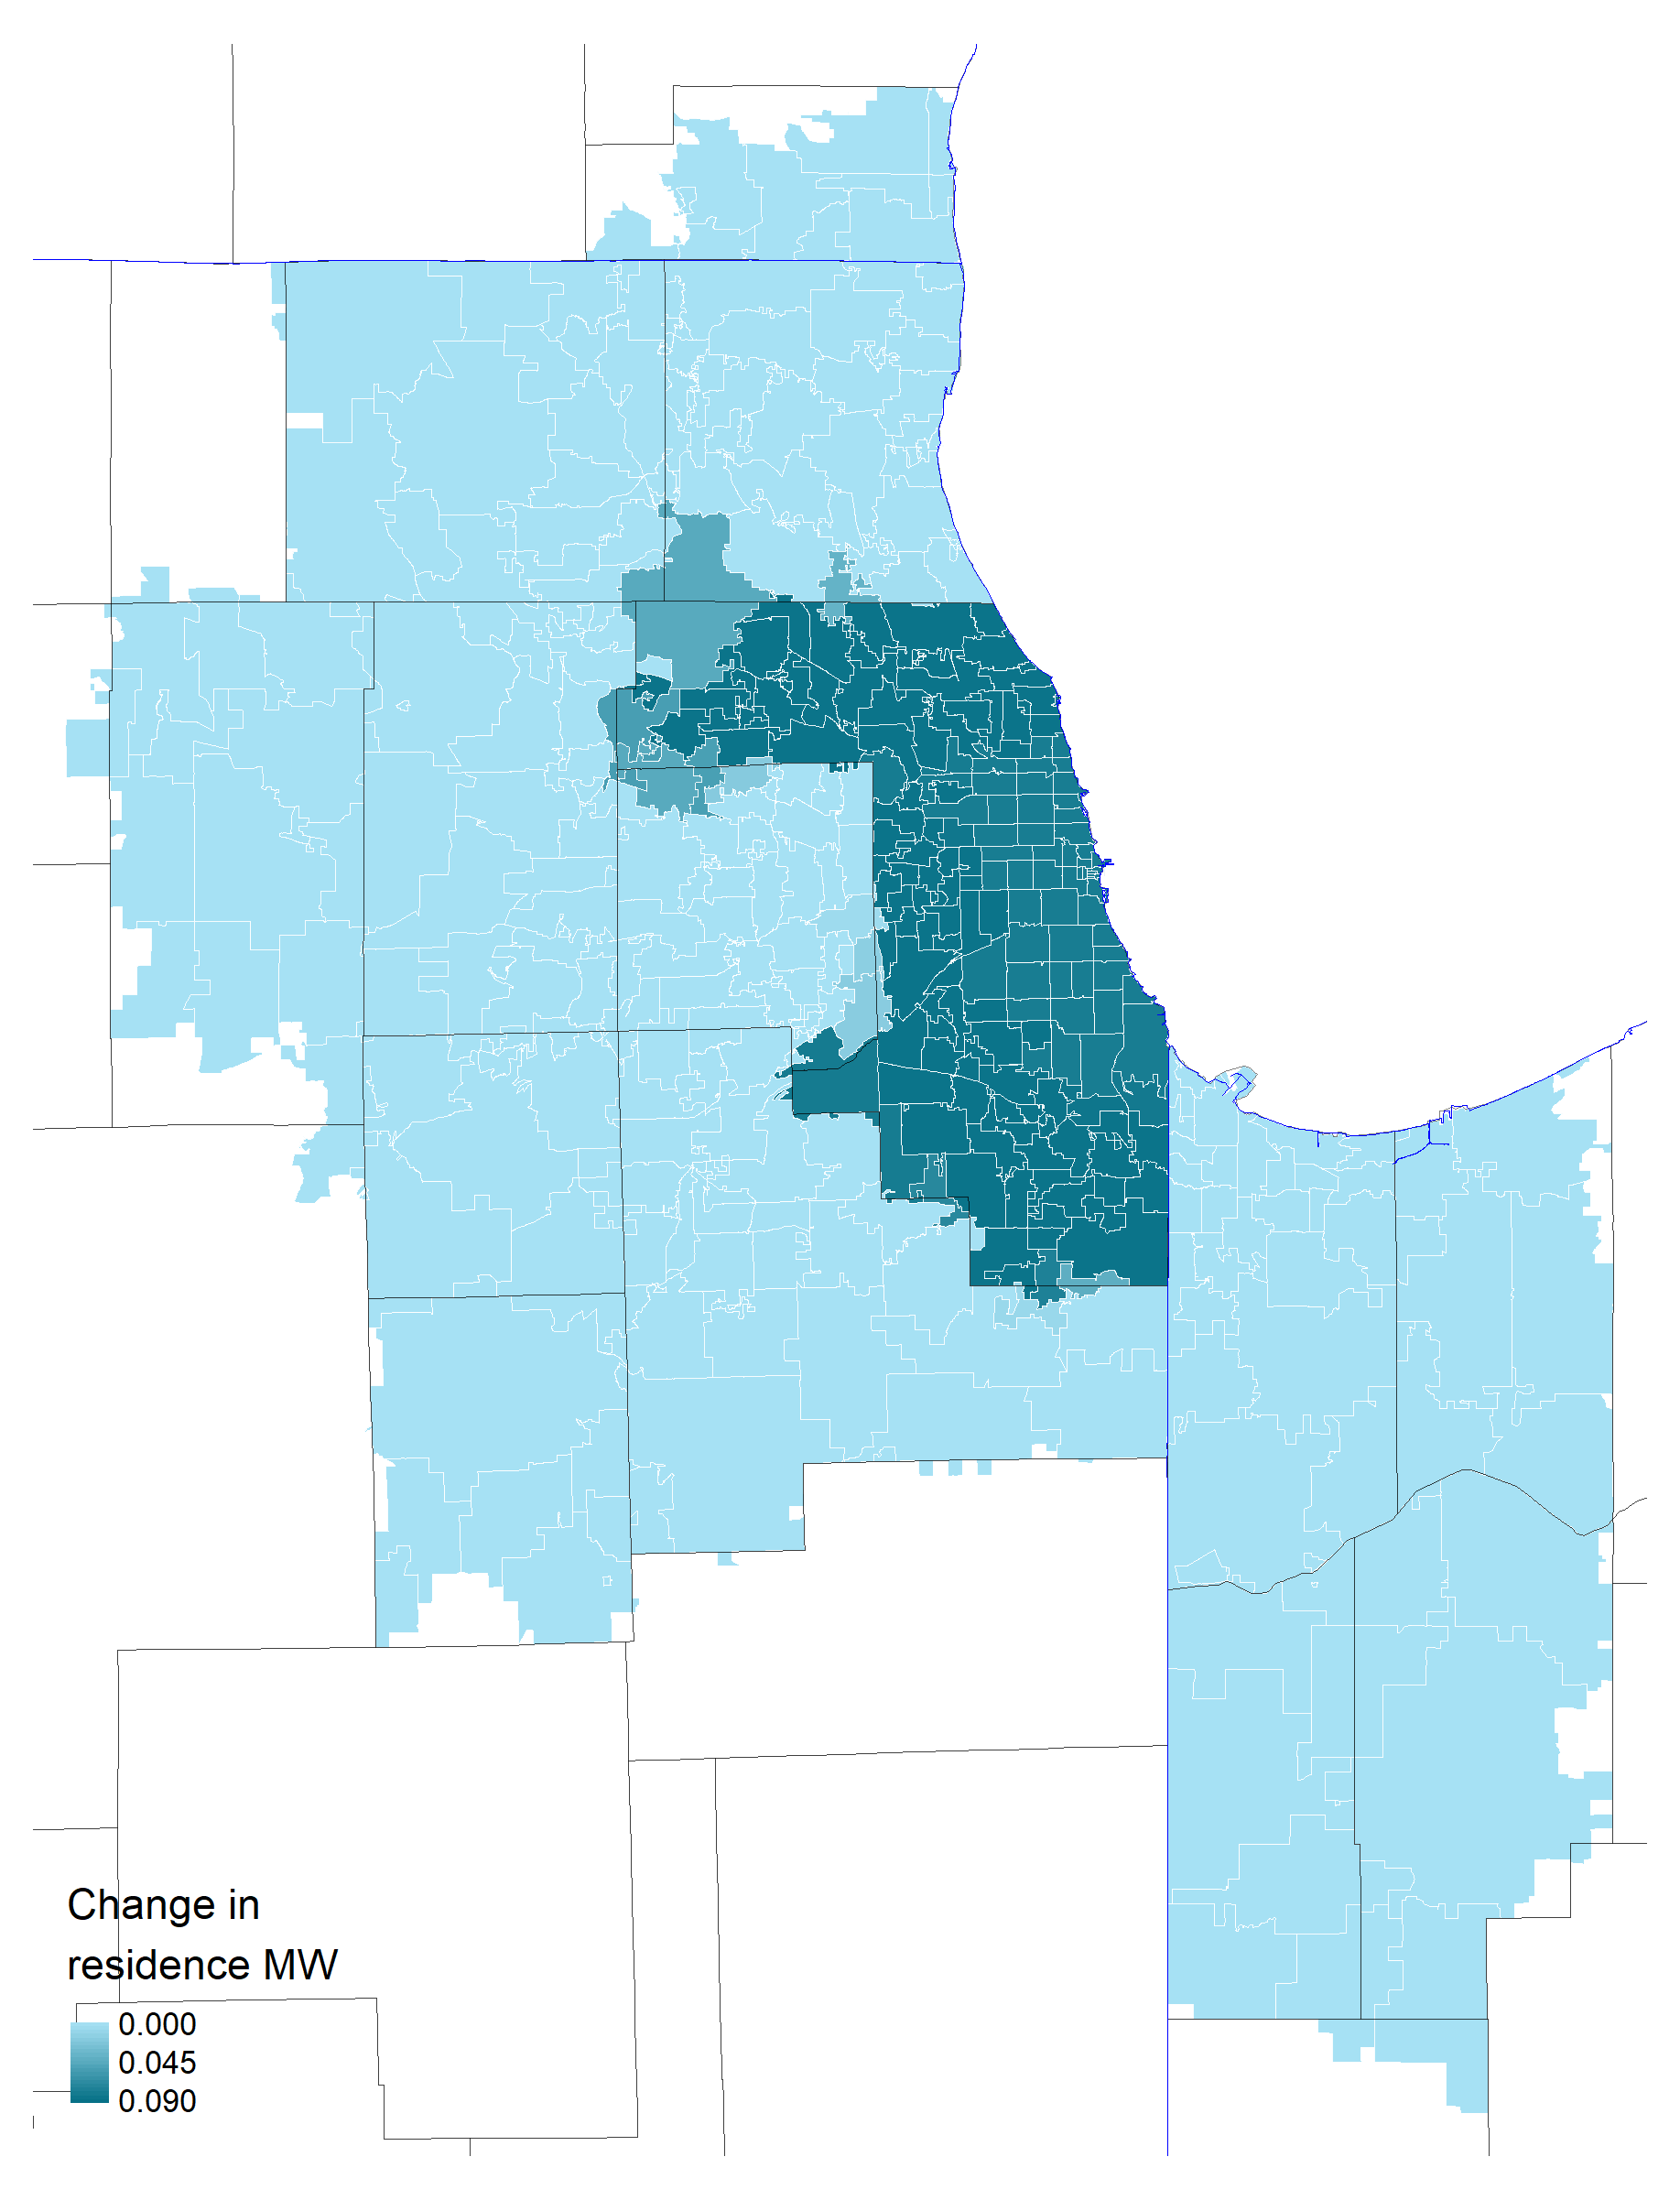
\includegraphics[scale = 0.38]{maps_events/output/chicago_2019-6_statutory_mw.png}
            \end{figure}   
        \end{column}
        \begin{column}{0.56\textwidth}
            Cook County, IL
            \begin{itemize}
                \item Raised local MW from \$12 to \$13 in July 2019. 
                \item State MW is \$8.25 since 2010, and federal MW is \$7.25 since 2009.
                \vspace{2mm}
                \pause
                \item A model where only same-location MW affects rents 
                would miss likely rents increases outside of Cook County
            \end{itemize}
        \end{column}
    \end{columns}
\end{frame}

\begin{frame}
\frametitle{A novel model-based measure of exposure to minimum wages}

    For ZIP code $i$ and month $t$ we define the {\color{blue} workplace MW} as
    $$
    {\color{blue} \mw^{\wkp}_{it}} = 
    \sum_{z \in \Z(i)} \pi_{i z} \ln \MW_{zt} \ ,
    $$
    %% IMPORTANT: We average the log of the MW! (Not log the average)
    \vspace{-2.5mm}
    where
    \vspace{1mm}
    \begin{itemize} \small
        \item $\MW_{zt}$ is statutory MW in $z$ at time $t$
        \item $\Z(i)$ are workplace locations of $i$'s residents
        \item $\pi_{i z} = L_{i z}/L_i$ is the share of $i$'s residents who work 
        in $z$
    \end{itemize}

    \vspace{3mm}
    The {\color{red} residence MW} is simply
    $$
    {\color{red} \mw^{\res}_{it}} = \ln \MW_{it}
    $$
\end{frame}

\begin{frame}[label = chi_example]
\frametitle{A motivating example (continuation)}
    \vspace{-6mm}
    \begin{columns}
        \begin{column}{0.50\textwidth}
            \vspace{-4mm}
            \begin{figure}
                \centering
                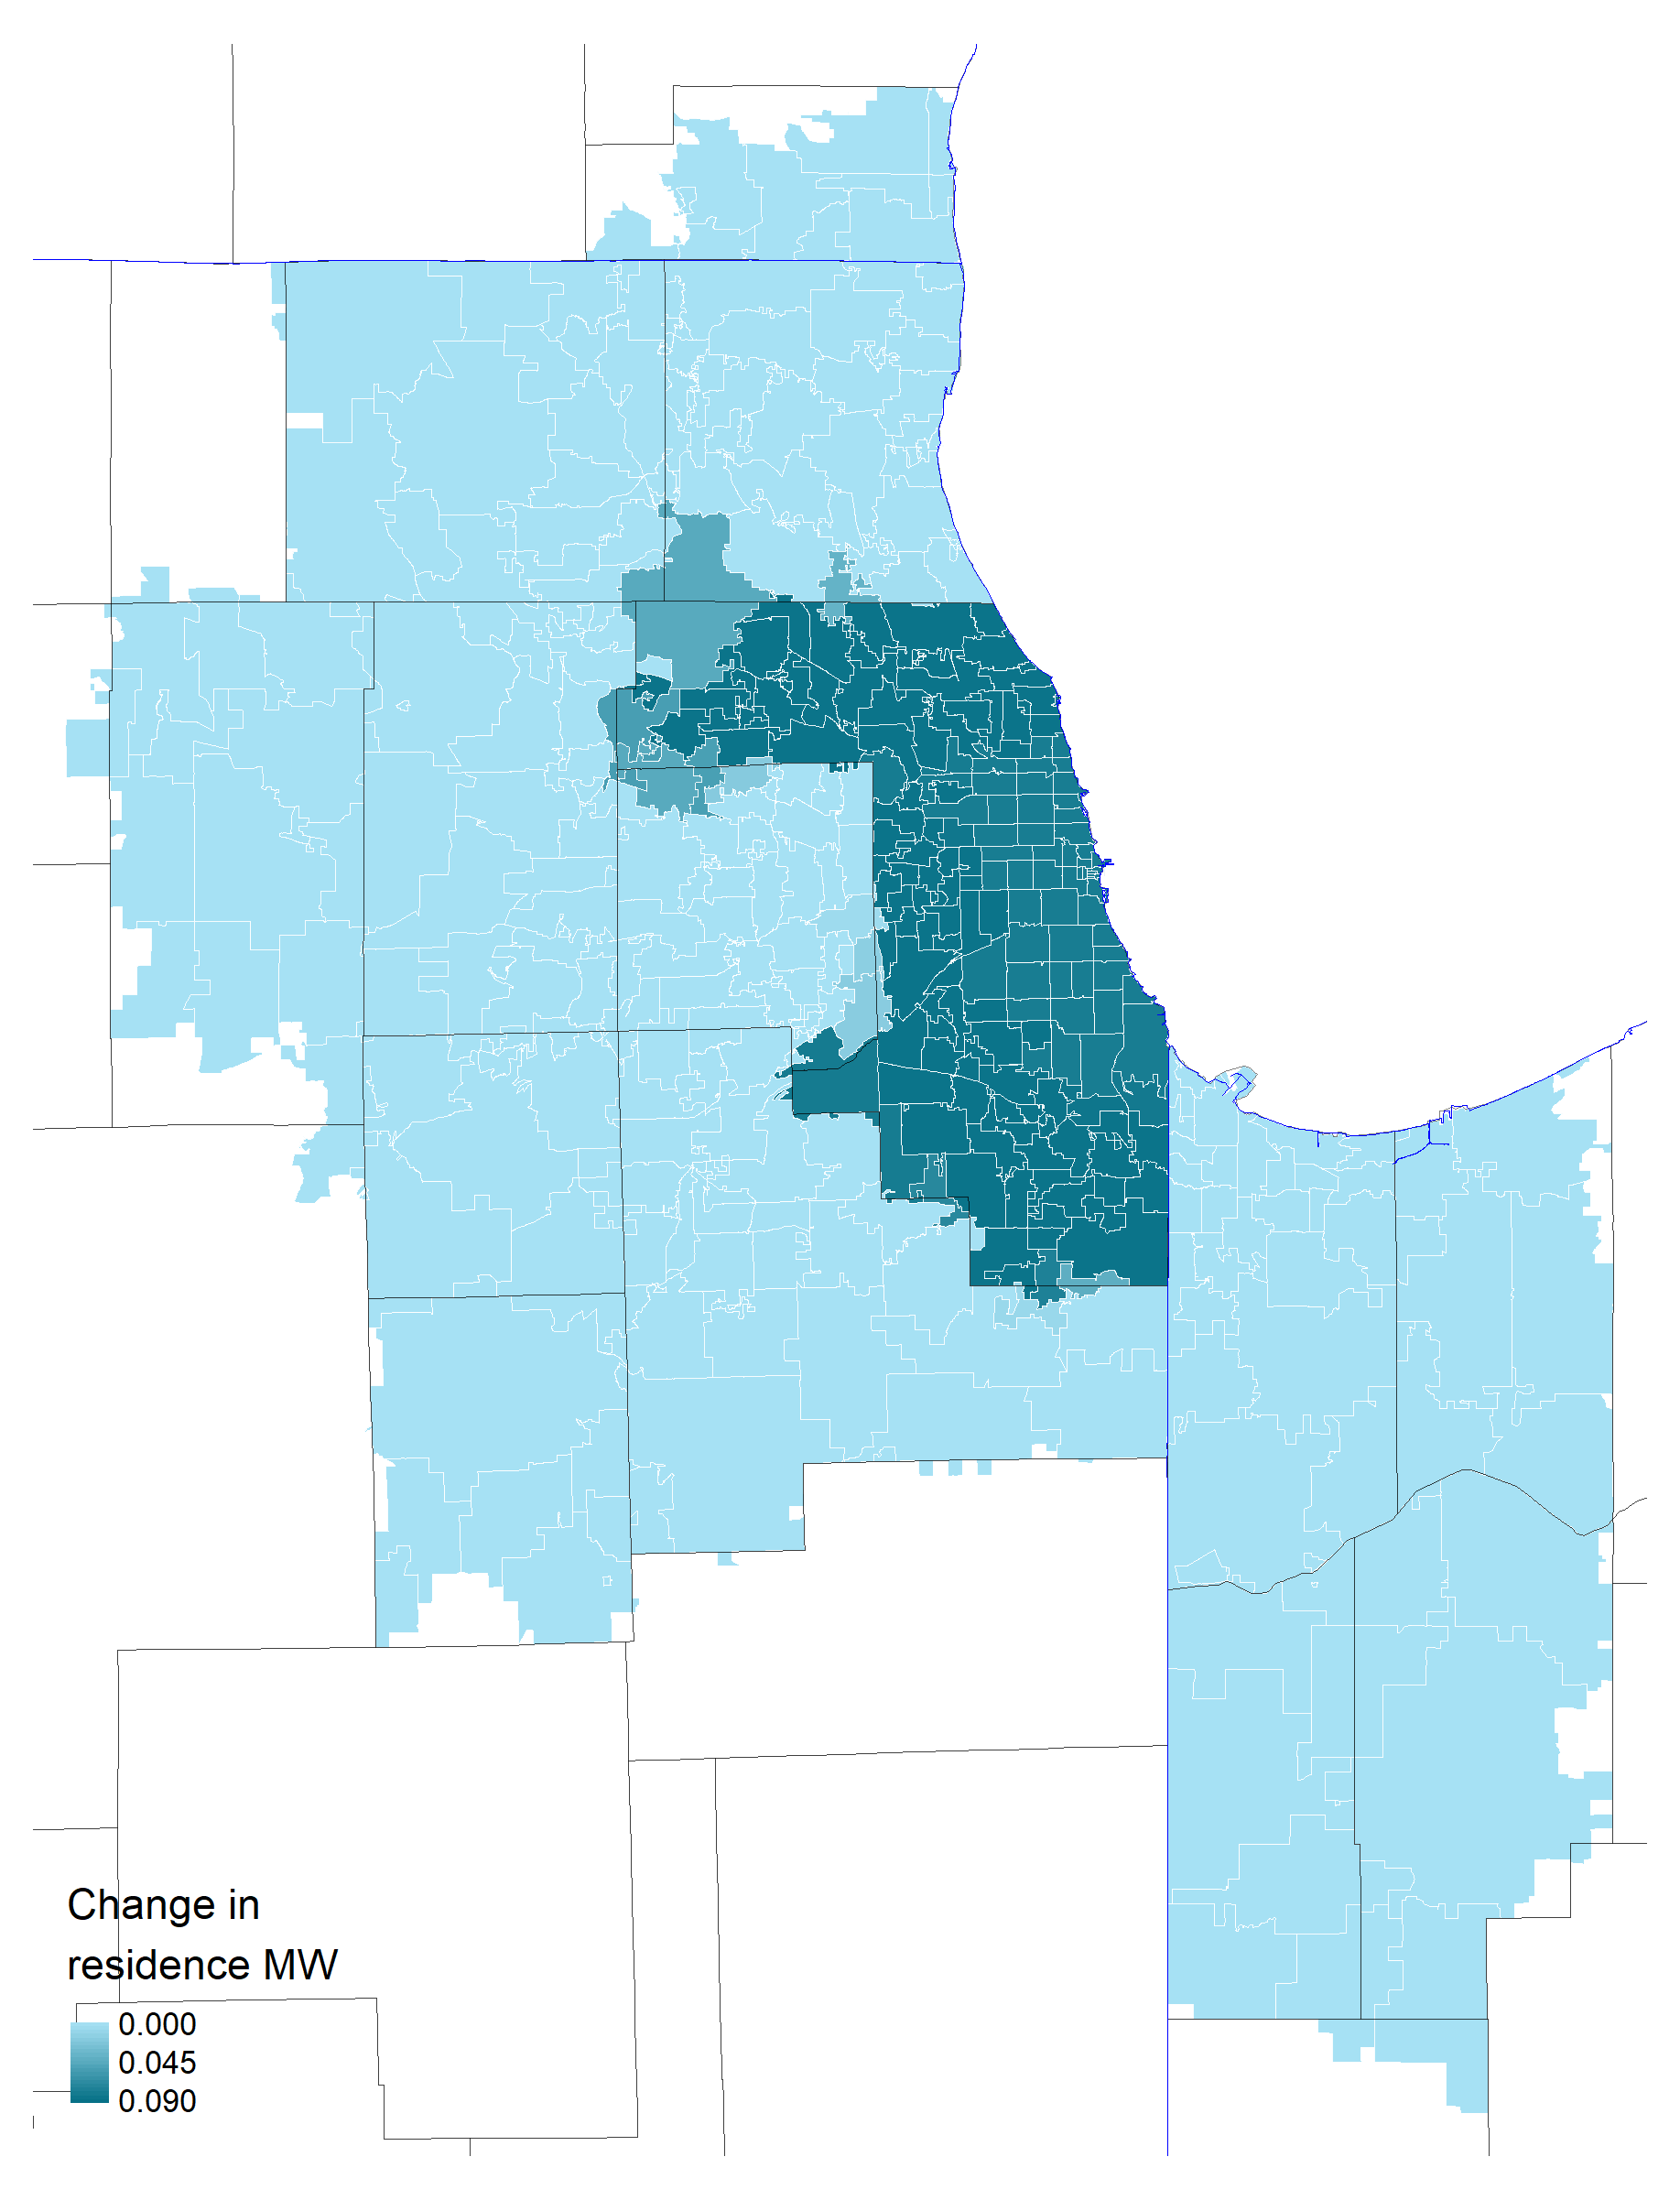
\includegraphics[scale = 0.35]{maps_events/output/chicago_2019-6_statutory_mw.png}
            \end{figure}   
        \end{column}
        \begin{column}{0.50\textwidth}
            \vspace{-4mm}
            \begin{figure}
                \centering
                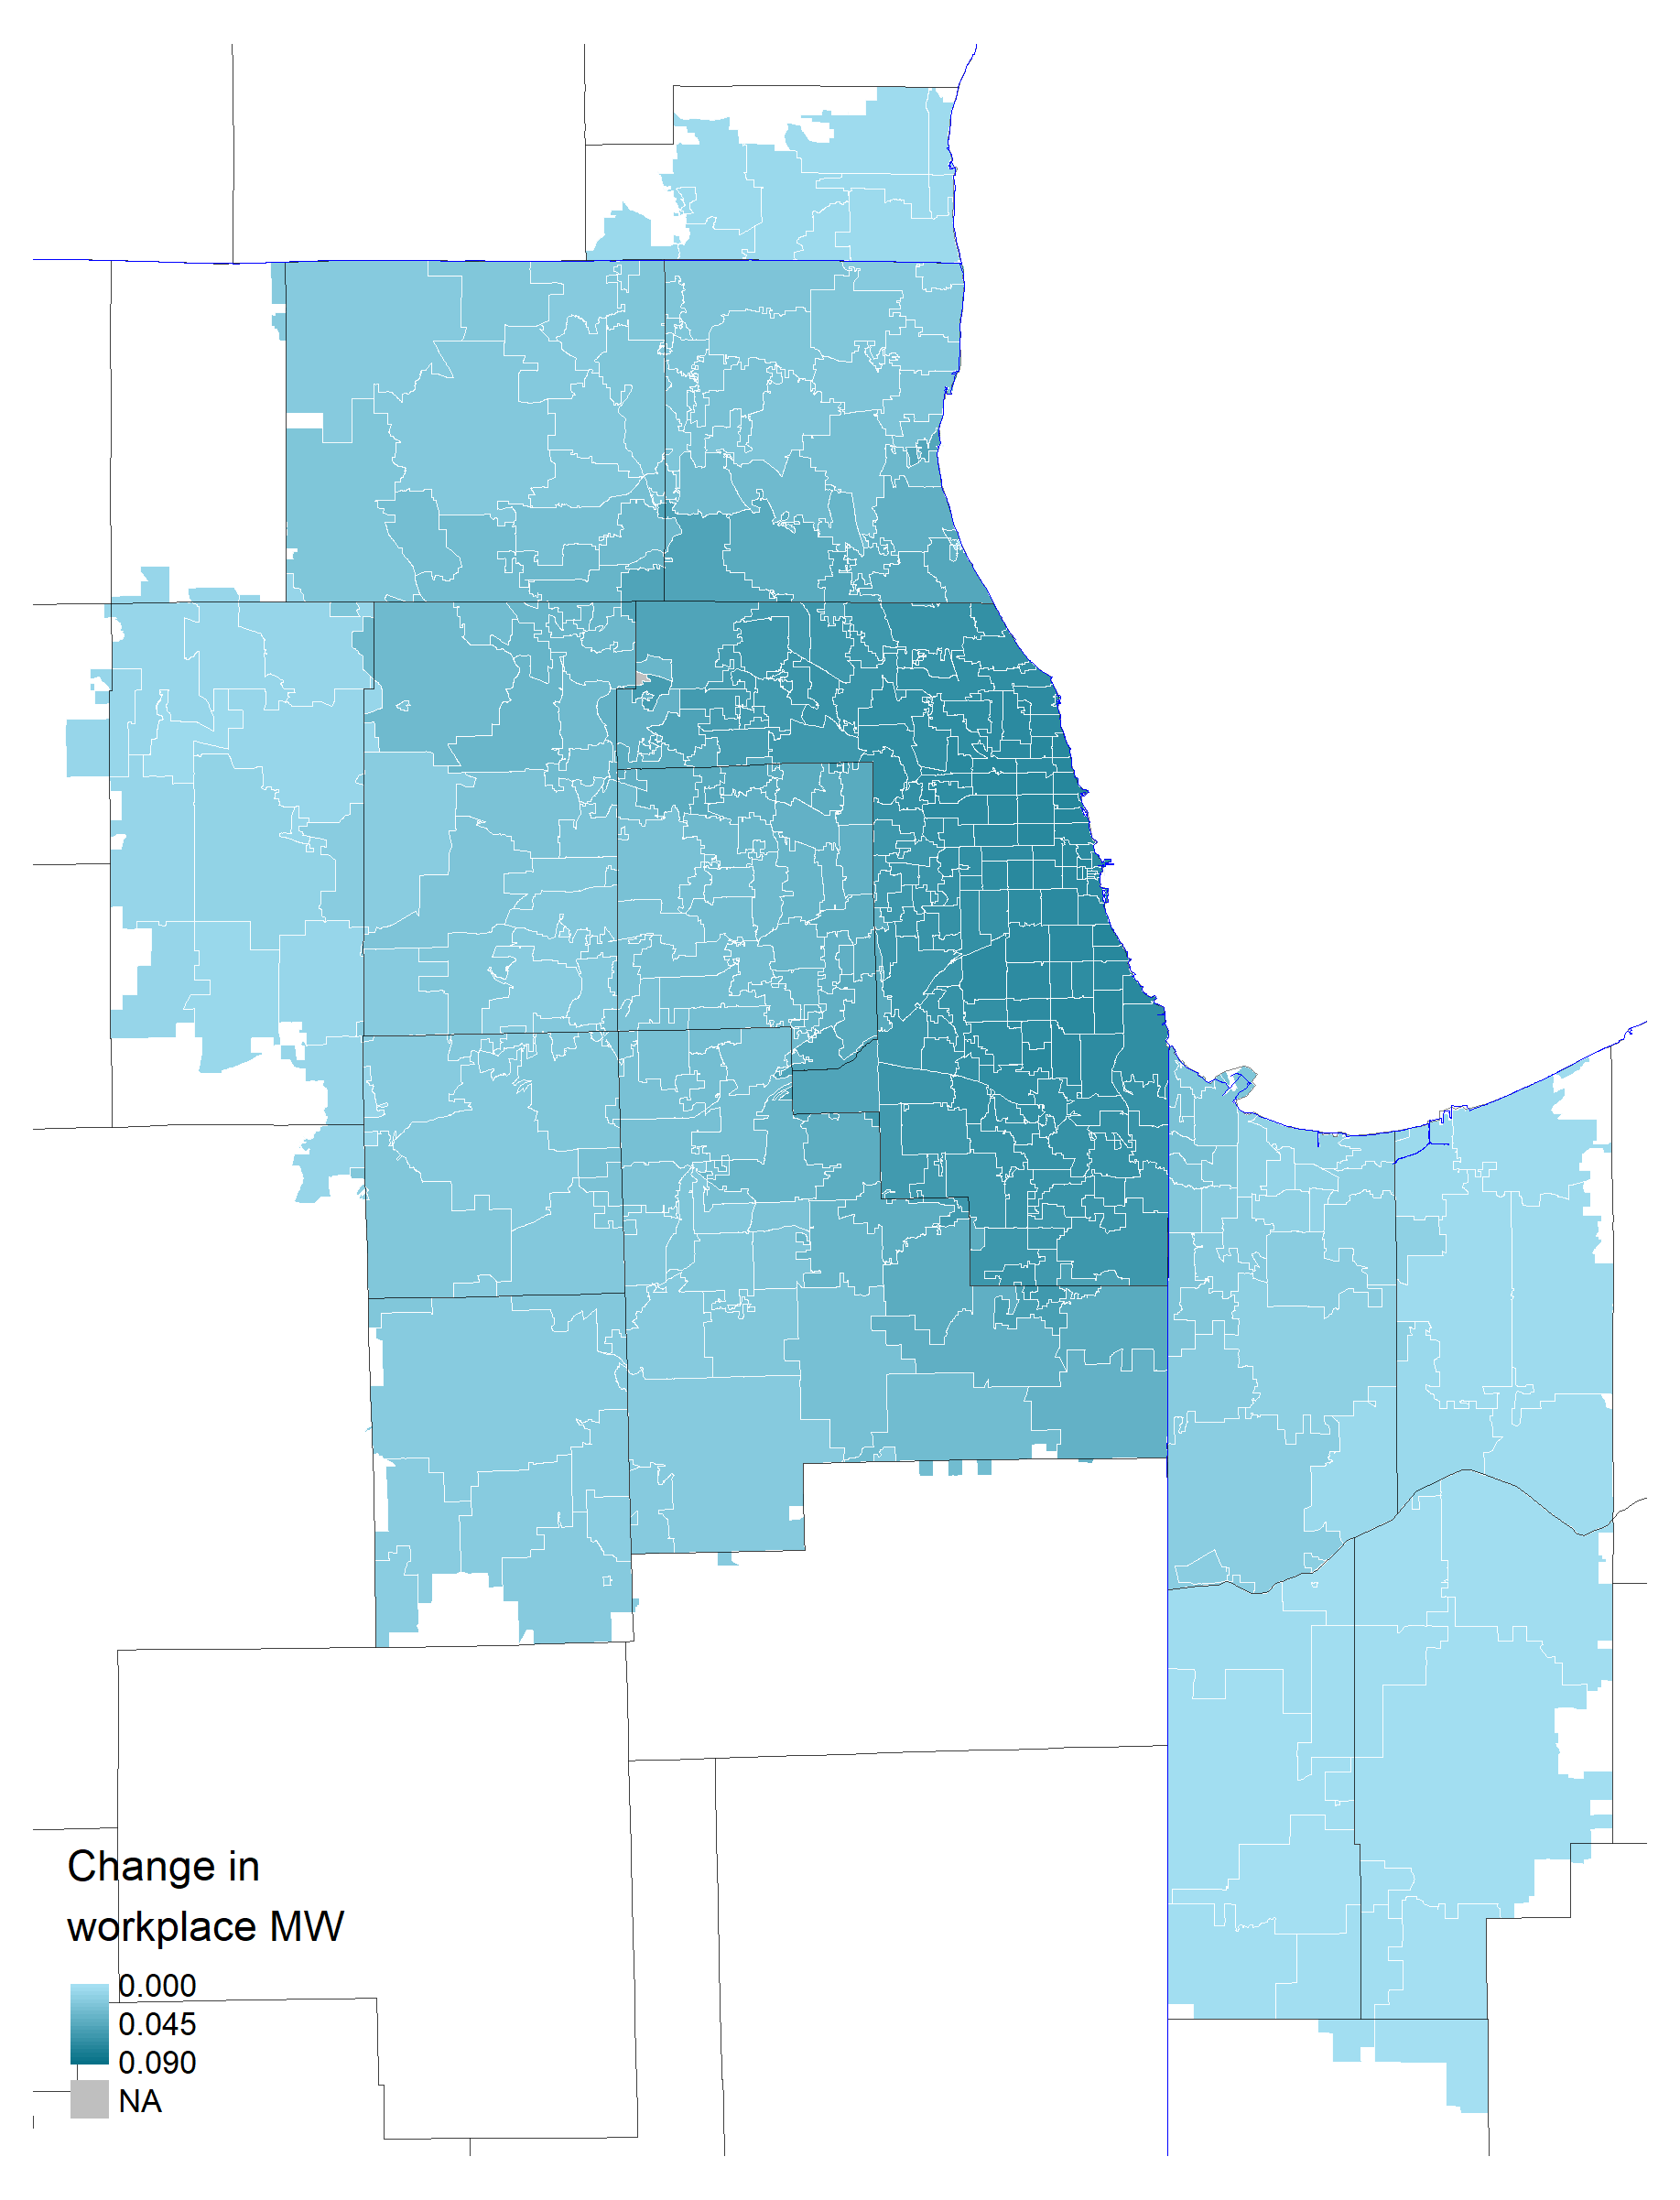
\includegraphics[scale = 0.35]{maps_events/output/chicago2019-6_wkp_mw.png}
            \end{figure}   
        \end{column}
    \end{columns}
    \vspace{3mm}
    \hyperlink{nyc_example}{\beamerbutton{NYC}} 
    \hyperlink{bay_example}{\beamerbutton{Bay Area}}
    \hyperlink{san_diego_example}{\beamerbutton{San Diego}}
    \hyperlink{kc_example}{\beamerbutton{Kansas City}}
\end{frame}

\begin{frame}
    \frametitle{Preview of findings}
    
    Main estimation results
    \begin{itemize}
        \vspace{1mm}
        \item 10 percent $\uparrow$ in {\color{blue} workplace MW}
        $\implies$ 0.55 percent $\uparrow$ in rents
        \vspace{1mm}
        \item 10 percent $\uparrow$ in {\color{red} residence MW}
        $\implies$ 0.21 percent $\downarrow$ in rents
        \vspace{1mm}
        \item 10 percent $\uparrow$ in both measures $\implies$ 0.34 percent $\uparrow$ in rents
    \end{itemize}
    %% Similar magnitude to estimates of MW effects on prices
    
    \vspace{5mm}
    \pause
    Counterfactual increase in federal MW from \$7.25 to \$9 in highly affected areas
    \begin{itemize}
        \vspace{1mm}
        \item Rent changes vary between $-0.4$ to $0.75$ percent (median $0.5$ percent)
        % A rental that costs 2000 would increase to 2100
        \vspace{1mm}
        \item Share pocketed by landlords is between $-15$ and $17$ cents (median $10$ cents)
    \end{itemize}
    %% Distribution are left skewed or negatively skewed
\end{frame}

\begin{frame}
    \frametitle{Outline for Today}
    \tableofcontents[hideallsubsections]
\end{frame}

%%%%%%%%%%%%%%%%%%%%%%%%%%%%%%%%%%%%%%%%%%%%%%%%%%%%%%%%%%%%%%%%%%%%%%%%%%%%%%%%
\section{Partial Equilibrium Model (intuition)}

\begin{frame}
    \frametitle{Overview}
    
    Goals of the model
    \begin{itemize}
        \item Stylized answer to what is the effect of MW changes on rents
        \item Motivate and derive a new measure of exposure to MW
    \end{itemize}
    
    \pause
    \vspace{3mm}
    Assumptions
    \begin{itemize}
        \item A higher MW increases income, which \textit{increases} housing demand
        \item A higher MW increases non-tradable, which \textit{decreases} housing demand
        \item Static model, so residence and workplace locations of workers are fixed
    \end{itemize}

    \vspace{1mm}
    These assumptions are consistent with the literature

\end{frame}

\begin{frame}
    \frametitle{Comparative statics}
    
    \begin{columns}
        \begin{column}{0.35\textwidth}
            \begin{enumerate}
                \item Equilibrium in ZIP code $i$
                \item \onslide<2->{\color{blue} MW increases in some $z$}
                \item \onslide<3->{\color{red} MW increases in $i$}
            \end{enumerate}
        \end{column}
        \begin{column}{0.65\textwidth}
            \vspace{-2mm}
            \begin{figure}

                \begin{tikzpicture}[scale=.95]
                
                % Axis
                \draw[->, thick] (0,0) -- (6.5,0);
                \draw[->, thick] (0,0) -- (0,6.2);
                \node[left] at (0.2,6.5) {Rents};
                \node[right] at (5,-0.5) {Square feet};
                
                % Base demand and Supply Curves
                \draw (0.3,4.5) -- (4.8,0.5);
                \draw plot [smooth, tension = 1] coordinates {(0.3,1.4) (3,2.8) (5,4.7)};
                       
                \node[right] at (4.8,0.5) {$H\left(R_i, P_i^0, \{Y_z^0\}\right)$};
                \node[right] at (5,4.7) {$S\left(R_i\right)$};
                
                % Base Eq
                \def\x{2.51}
                \def\y{2.5}
                \draw[dashed] (\x,0) -- (\x,\y);
                \draw[dashed] (0,\y) -- (\x,\y);
                \node[below] at (\x,0) {$H_0^*$};
                \node[left] at (0,\y) {$R_0^*$};
                
                % Equilibrium 1 - Wkp MW increases
                \def\xOne{3.53}
                \def\yOne{3.22}
                \only<2>{
                \draw[color = blue] (0.3,6.1) -- (4.8,2.1);
                \node[right] at (4.8,2.1) {$H\left(R_i, P_i^0, {\color{blue}\{Y_z^1\}}\right)$};

                \draw[dashed, color = blue] (\xOne,0) -- (\xOne,\yOne);
                \draw[dashed, color = blue] (0,\yOne) -- (\xOne,\yOne);
                \node[below, color = blue] at (\xOne,0) {$H_1^*$};
                \node[left, color = blue] at (0, \yOne) {$R_1^*$};
                }

                % Equilibrium 1 - Res MW increases
                \def\xTwo{3.07}
                \def\yTwo{2.85}
                \only<3>{
                \draw[dashed, color = blue] (0.3,6.1) -- (4.8,2.1);
                \draw[color = red] (0.3,5.3) -- (4.8,1.3);
                \node[right] at (4.8,1.3) {$H\left(R_i, {\color{red}P_i^2}, {\color{red}\{Y_z^2\}}\right)$};

                \draw[dashed, color = blue] (\xOne,0) -- (\xOne,\yOne);
                \draw[dashed, color = blue] (0,\yOne) -- (\xOne,\yOne);
                \node[below, color = blue] at (\xOne+.3,0) {$H_1^*$};
                \node[left, color = blue] at (0, \yOne+.4) {$R_1^*$};

                \draw[dashed, color = red] (\xTwo,0) -- (\xTwo,\yTwo);
                \draw[dashed, color = red] (0,\yTwo) -- (\xTwo,\yTwo);
                \node[below, color = red] at (\xTwo,0) {$H_2^*$};
                \node[left, color = red] at (0,\yTwo+.2) {$R_2^*$};
                }
                
                \end{tikzpicture}
                
            \end{figure}
        \end{column}
    \end{columns}

\end{frame}

\begin{frame}
    \frametitle{Representation}

    In this model, assuming homogeneity across workplace locations of
    \begin{enumerate}
        \item elasticity of per-person housing demand to income, and
        \item elasticity of income to the MW
    \end{enumerate}
    we obtain
    \[
    \begin{split}
        \Delta \text{log rents} & = \beta_i  \times \Delta {\color{blue}  \text{workplace MW}} \\
                                & + \gamma_i \times \Delta {\color{red} \text{residence MW}} \\
    \end{split}
    \]

    \vspace{3mm}
    \pause
    Discussion:
    \begin{itemize}
        \item Assumption (1) would hold for homothetic preferences
        \item In estimation can allow for heterogeneity as long as not correlated with MW changes
    \end{itemize}

\end{frame}


%%%%%%%%%%%%%%%%%%%%%%%%%%%%%%%%%%%%%%%%%%%%%%%%%%%%%%%%%%%%%%%%%%%%%%%%%%%%%%%%
\section{Data}

\begin{frame}[label = zillow_data]
    \frametitle{Zillow Data}
    
    \begin{itemize}
        \item Leader online real estate and rental platform in the U.S. {\small (more 
        than 110 million homes and 170 million unique monthly users in 2019).}
        
        \vspace{2mm} \item
        Provides \textit{median} rents data at ZIP code, county, and state levels 
        at a monthly frequency for several housing categories.
        
        \pause
        \vspace{2mm} \item
        We use category single-family, condominium, and cooperative houses (SFCC).
        \begin{itemize}
            \item Most populated series in Zillow
            \item We also estimate our models with other housing categories
        \end{itemize}
        
        \vspace{2mm} \item
        Limitation: Zillow sample is not random.

        \hyperlink{zillow_pop_density}{\beamerbutton{Zillow ZIP Codes and Population Density}}

    \end{itemize}
\end{frame}

\begin{frame}[label=stat_MW]
    \frametitle{The Statutory MW}
    
    \begin{itemize}
        \item
        Collect MW data at state, county and city levels between Jan 2010 and Dec 2019.
        
        \vspace{2mm}
        \item
        Spatial match:
        \begin{itemize}
            \item Assign census blocks to USPS ZIP codes based on blocks' centroids
            \item Add matching of places, counties, and states using census crosswalk
        \end{itemize}
        
        \vspace{2mm}
        \item
        Assign MWs to each block and define statutory MW as maximum between city, county, state, and federal level.
        
        \vspace{2mm}
        \item
        Define statutory MW in ZIP code $i$ and month $t$, $\MW_{it}$, as weighted
        average of statutory MWs at block, using housing units as weights.

    \end{itemize}
    
\end{frame}

\begin{frame}[label=dist_mw_changes]
    \frametitle{Distribution of (positive) MW changes}

    \vspace{-4mm}
    \begin{figure}
        \begin{subfigure}{0.51\textwidth}
            \vspace{6mm}
            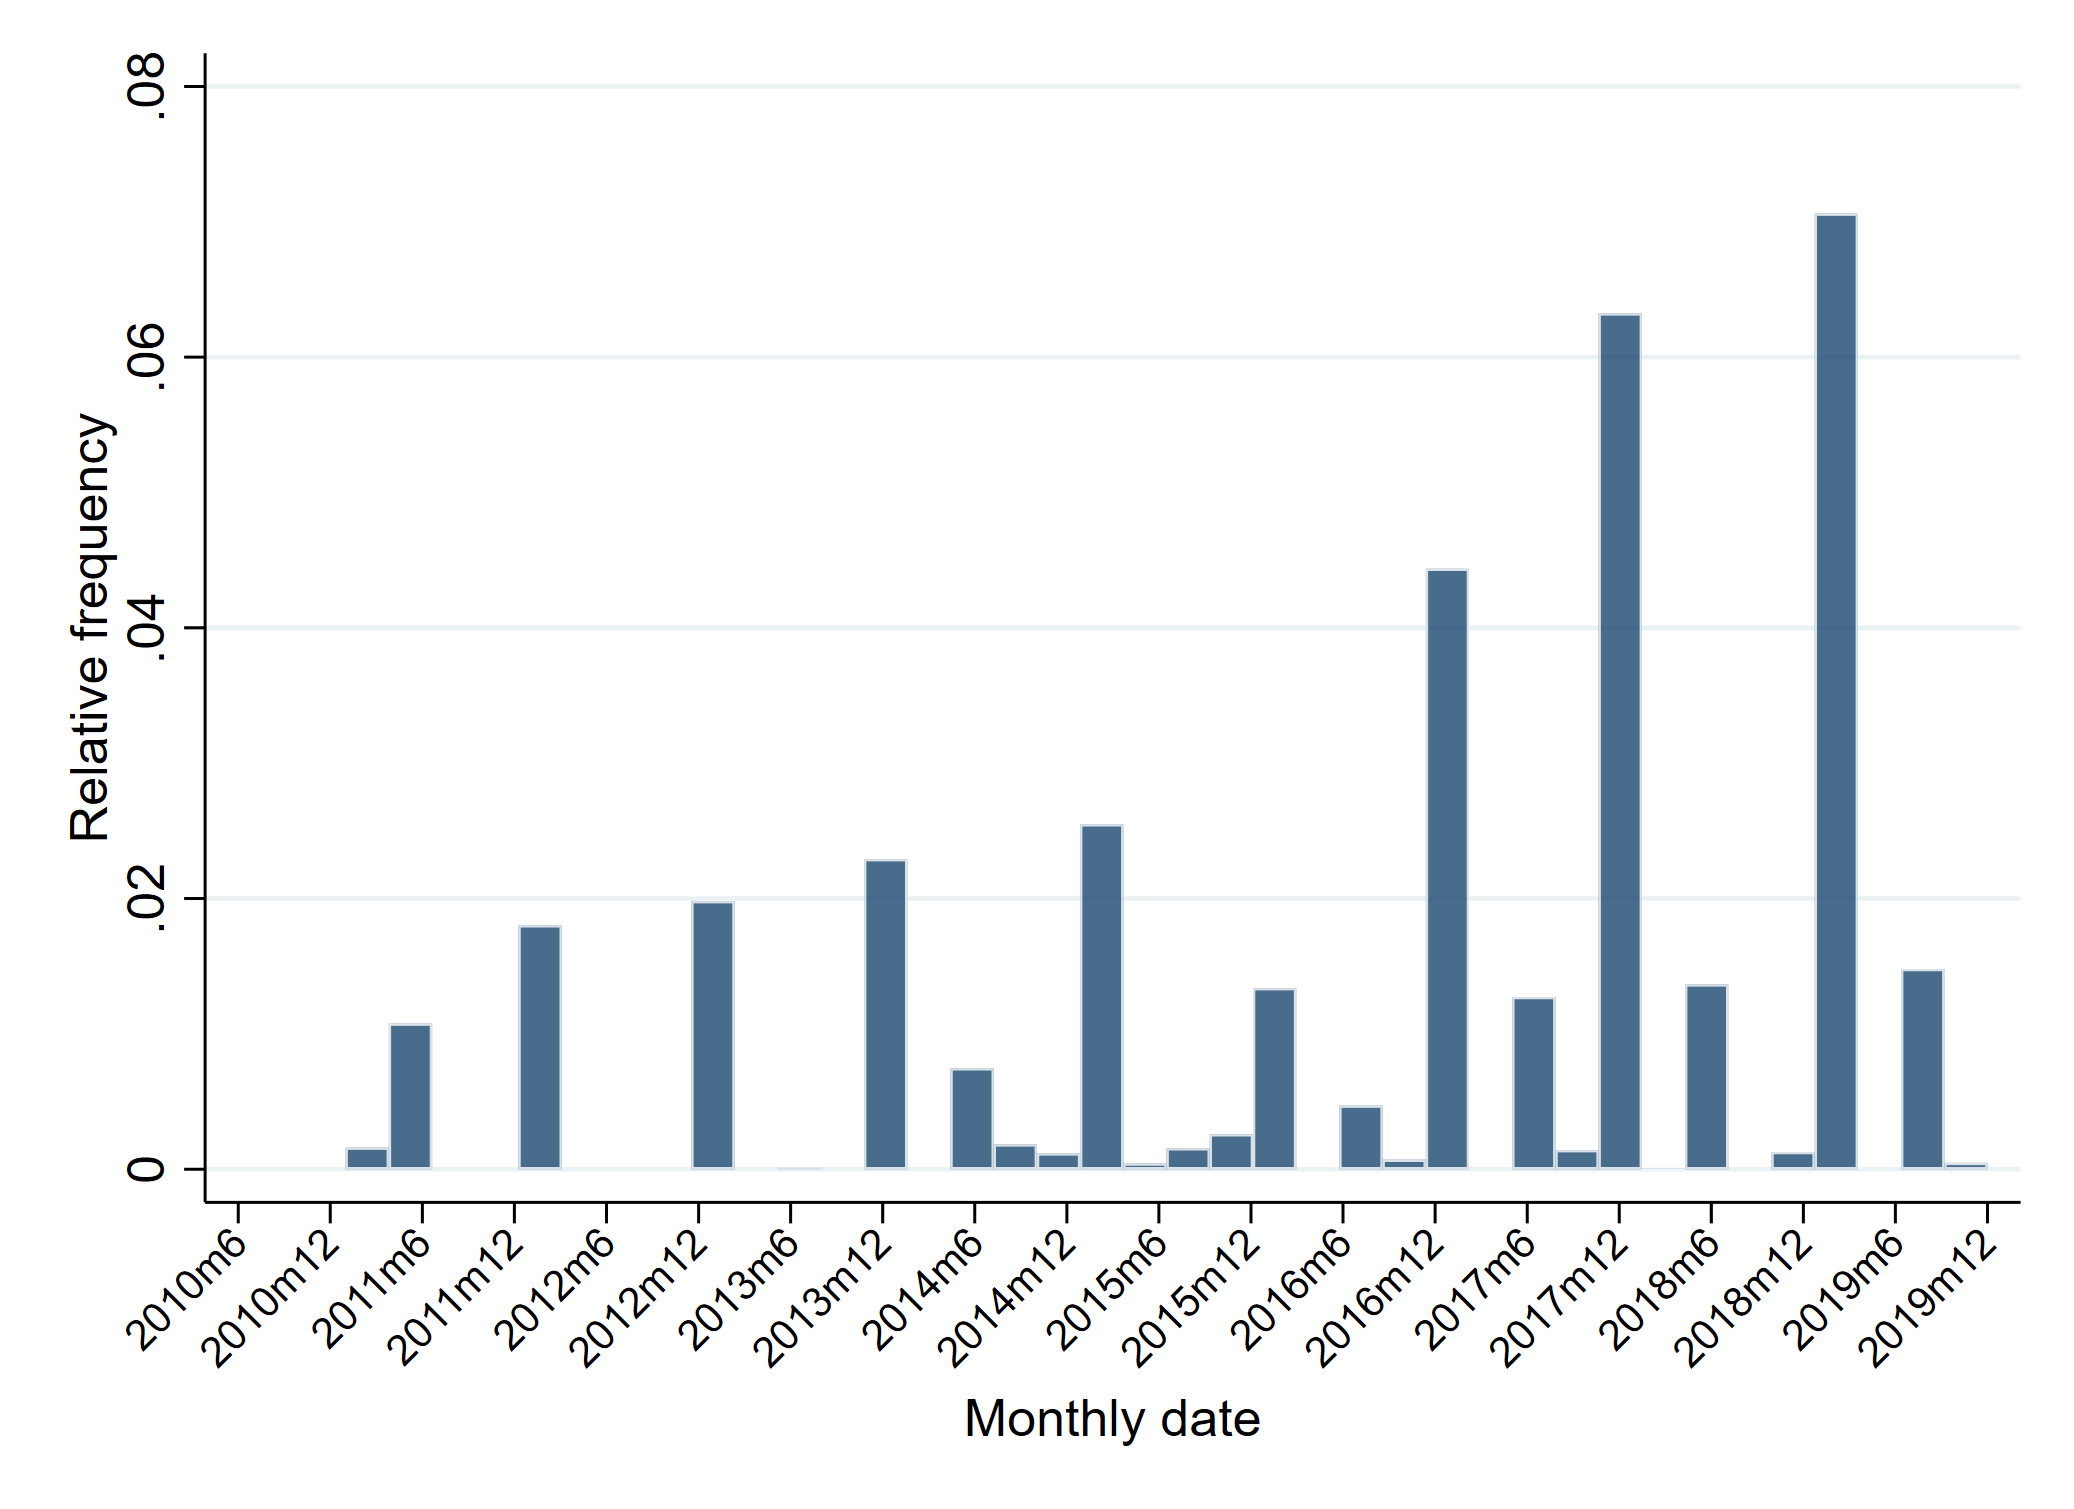
\includegraphics[width = 1.02\textwidth]{estimation_samples/output/pct_ch_mw_date_dist.png}
        \end{subfigure}%
        \begin{subfigure}{0.51\textwidth}
            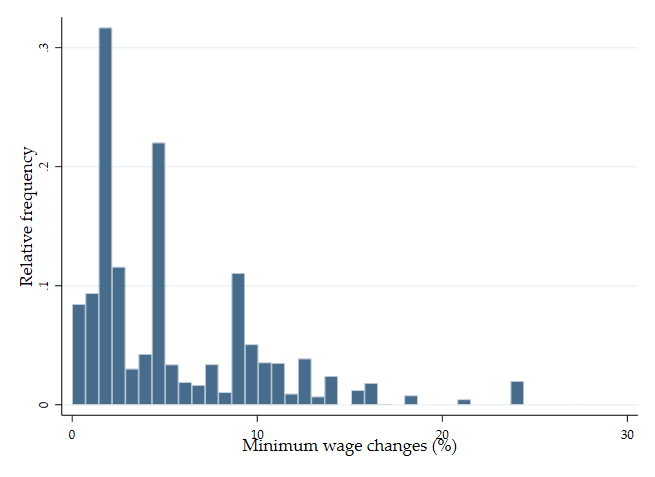
\includegraphics[width = 1.02\textwidth]{estimation_samples/output/pct_ch_mw_dist.png}
        \end{subfigure}
    \end{figure}
    
    \hyperlink{mw_changes_map}{\beamerbutton{US map of MW changes}}
\end{frame}

\subsection{MW measures}

\begin{frame}
    \frametitle{Constructing the MW measures}
        
    Collect data from LEHD Origin-Destination Employment Statistics (LODES) for years 2009--18.
    \begin{itemize}
        \item Origin-destination matrices at block level constructed from tax records
    \end{itemize}

    \vspace{1mm}
    Construct \textbf{origin-destination matrix} at ZIP code level using spatial match.
    
    \pause
    \vspace{2mm}
    We observe:
    \begin{itemize} \small
        \item Number of workers residing in a ZIP code and working in every other ZIP code
        \item Analogous matrix for number of workers aged less than 29 and earning less than 
        \$1,251
    \end{itemize}
    
    \vspace{1mm}
    In our baseline specification we use constant commuter shares from 2017.
    \begin{itemize} \small
        \item Results are robust to using other years and groups
    \end{itemize}

    \pause
    \vspace{4mm}
    Define the MW measures as
    $$
    {\color{blue} \mw^{\wkp}_{it}} = \sum_{z \in \Z(i)} \pi_{i z} \ln \MW_{zt}
    \quad\quad\text{and}\quad\quad
    {\color{red} \mw^{\res}_{it}} = \ln \MW_{it}
    $$
\end{frame}

%%%%%%%%%%%%%%%%%%%%%%%%%%%%%%%%%%%%%%%%%%%%%%%%%%%%%%%%%%%%%%%%%%%%%%%%%%%%%%%%
\section{Empirical Strategy and Results}

\begin{frame}
    \frametitle{Empirical model}
        
    We estimate versions of the following empirical model:
    $$
    \Delta r_{it} = \delta_t +
        \beta \Delta {\color{blue}\mw^{\wkp}_{it}} +
        \gamma \Delta {\color{red}\mw^{\res}_{it}} + 
        \Delta \mathbf{X}^{'}_{it} \eta + 
        \Delta \varepsilon_{it} ,
    $$    
    where
    \begin{itemize}
        \item $r_{it} = \ln R_{it}$
        \item $\mathbf{X}^{'}_{it}$ are time-varying controls at the county level
    \end{itemize}
    
    \pause
    \vspace{4mm}
    For causal effect of $\beta$ and $\gamma$ we need:
    \begin{itemize}
        \item (Rank) Independent variation in MW measures after conditioning on controls
        \item (Parallel trends) Identification assumption:
        $$
        E\left[
            \begin{pmatrix}
                \Delta {\color{blue}\mw^{\wkp}_{is}} \\
                \Delta {\color{red}\mw^{\res}_{is}} \\
            \end{pmatrix}
            \Delta \varepsilon_{it}
        \bigg| \delta_t, \Delta \mathbf{X}_{it} \right] =
        \begin{pmatrix}
            0 \\
            0 \\
        \end{pmatrix}
        \quad \forall s
        $$
    \end{itemize}

\end{frame}

\begin{frame}[label = dyn_model]
    \frametitle{Identification assumption concerns}
    
    MW policies are rarely set by considering differential dynamics of the 
    rental housing market within metropolitan areas.
    %% For example, the Congressional Budget Office (CBO) doesn't mention rents even 
    %% once in it's study of the effects of the Wage Act of 2021
    %% https://www.cbo.gov/system/files/2021-02/56975-Minimum-Wage.pdf
    \begin{itemize}
        \item Even more true for small geographies such as ZIP codes
    \end{itemize}

    \vspace{2mm}
    \pause
    We extend our model adding leads and lags to test for parallel trends
    $$
    \Delta r_{it} = \delta_t +
        \sum_{k=-s}^{s} \beta {\color{blue}\Delta \mw^{\wkp}_{i,t+k}} +
        \sum_{k=-s}^{s} \gamma {\color{red} \Delta \mw^{\res}_{i,t+k}} + 
        \Delta \mathbf{X}^{'}_{it} \eta + 
        \Delta \varepsilon_{it} ,
    $$

    \vspace{2mm}
    We discuss other robustness checks later.
\end{frame}

\begin{frame}[label = static]
    \frametitle{Main results}

    \begin{table}
    \label{tab:static}
    \scalebox{0.8}{
        \begin{tabular}{l*{4}{c}}
            \toprule
            & \multicolumn{1}{c}{\shortstack{Change wkp.\ MW\\$\Delta\mw_{it}^{\wkp}$}}
                & \multicolumn{3}{c}{\shortstack{Change log rents\\$\Delta r_{it}$}} \\ \cmidrule(lr){2-2}\cmidrule(lr){3-5}
                                               & (1)   & (2)   & (3)   & (4)            \\ \midrule
            Change residence MW 
                      $\Delta\mw_{it}^{\res}$  &  #4#  &  #4#  &       &  #4#     \\
                                               & (#4#) & (#4#) &       & (#4#)    \\
            Change workplace MW 
                       $\Delta\mw_{it}^{\wkp}$ &       &       &  #4#  & #4#      \\
                                               &       &       & (#4#) & (#4#)    \\ \midrule
            Sum of coefficients                &       &       &       &  #4#     \\
                                               &       &       &       & (#4#)    \\ \midrule
            County-quarter economic controls   &  Yes  & Yes   & Yes   & Yes      \\
            P-value equality                   &       &       &       & #4#      \\
            R-squared                          &  #4#  &  #4#  &  #4#  & #4#      \\
            Observations                       & #0,#  & #0,#  & #0,#  & #0,#     \\\bottomrule
        \end{tabular}
    }
\end{table}

    
    \vspace{2mm}
    \footnotesize
    Note: Standard errors clustered at the state level throughout.

\end{frame}

\begin{frame}[label = dyn_baseline_plot]
    \frametitle{Including leads and lags of workplace MW}

    \begin{figure}
        \centering
        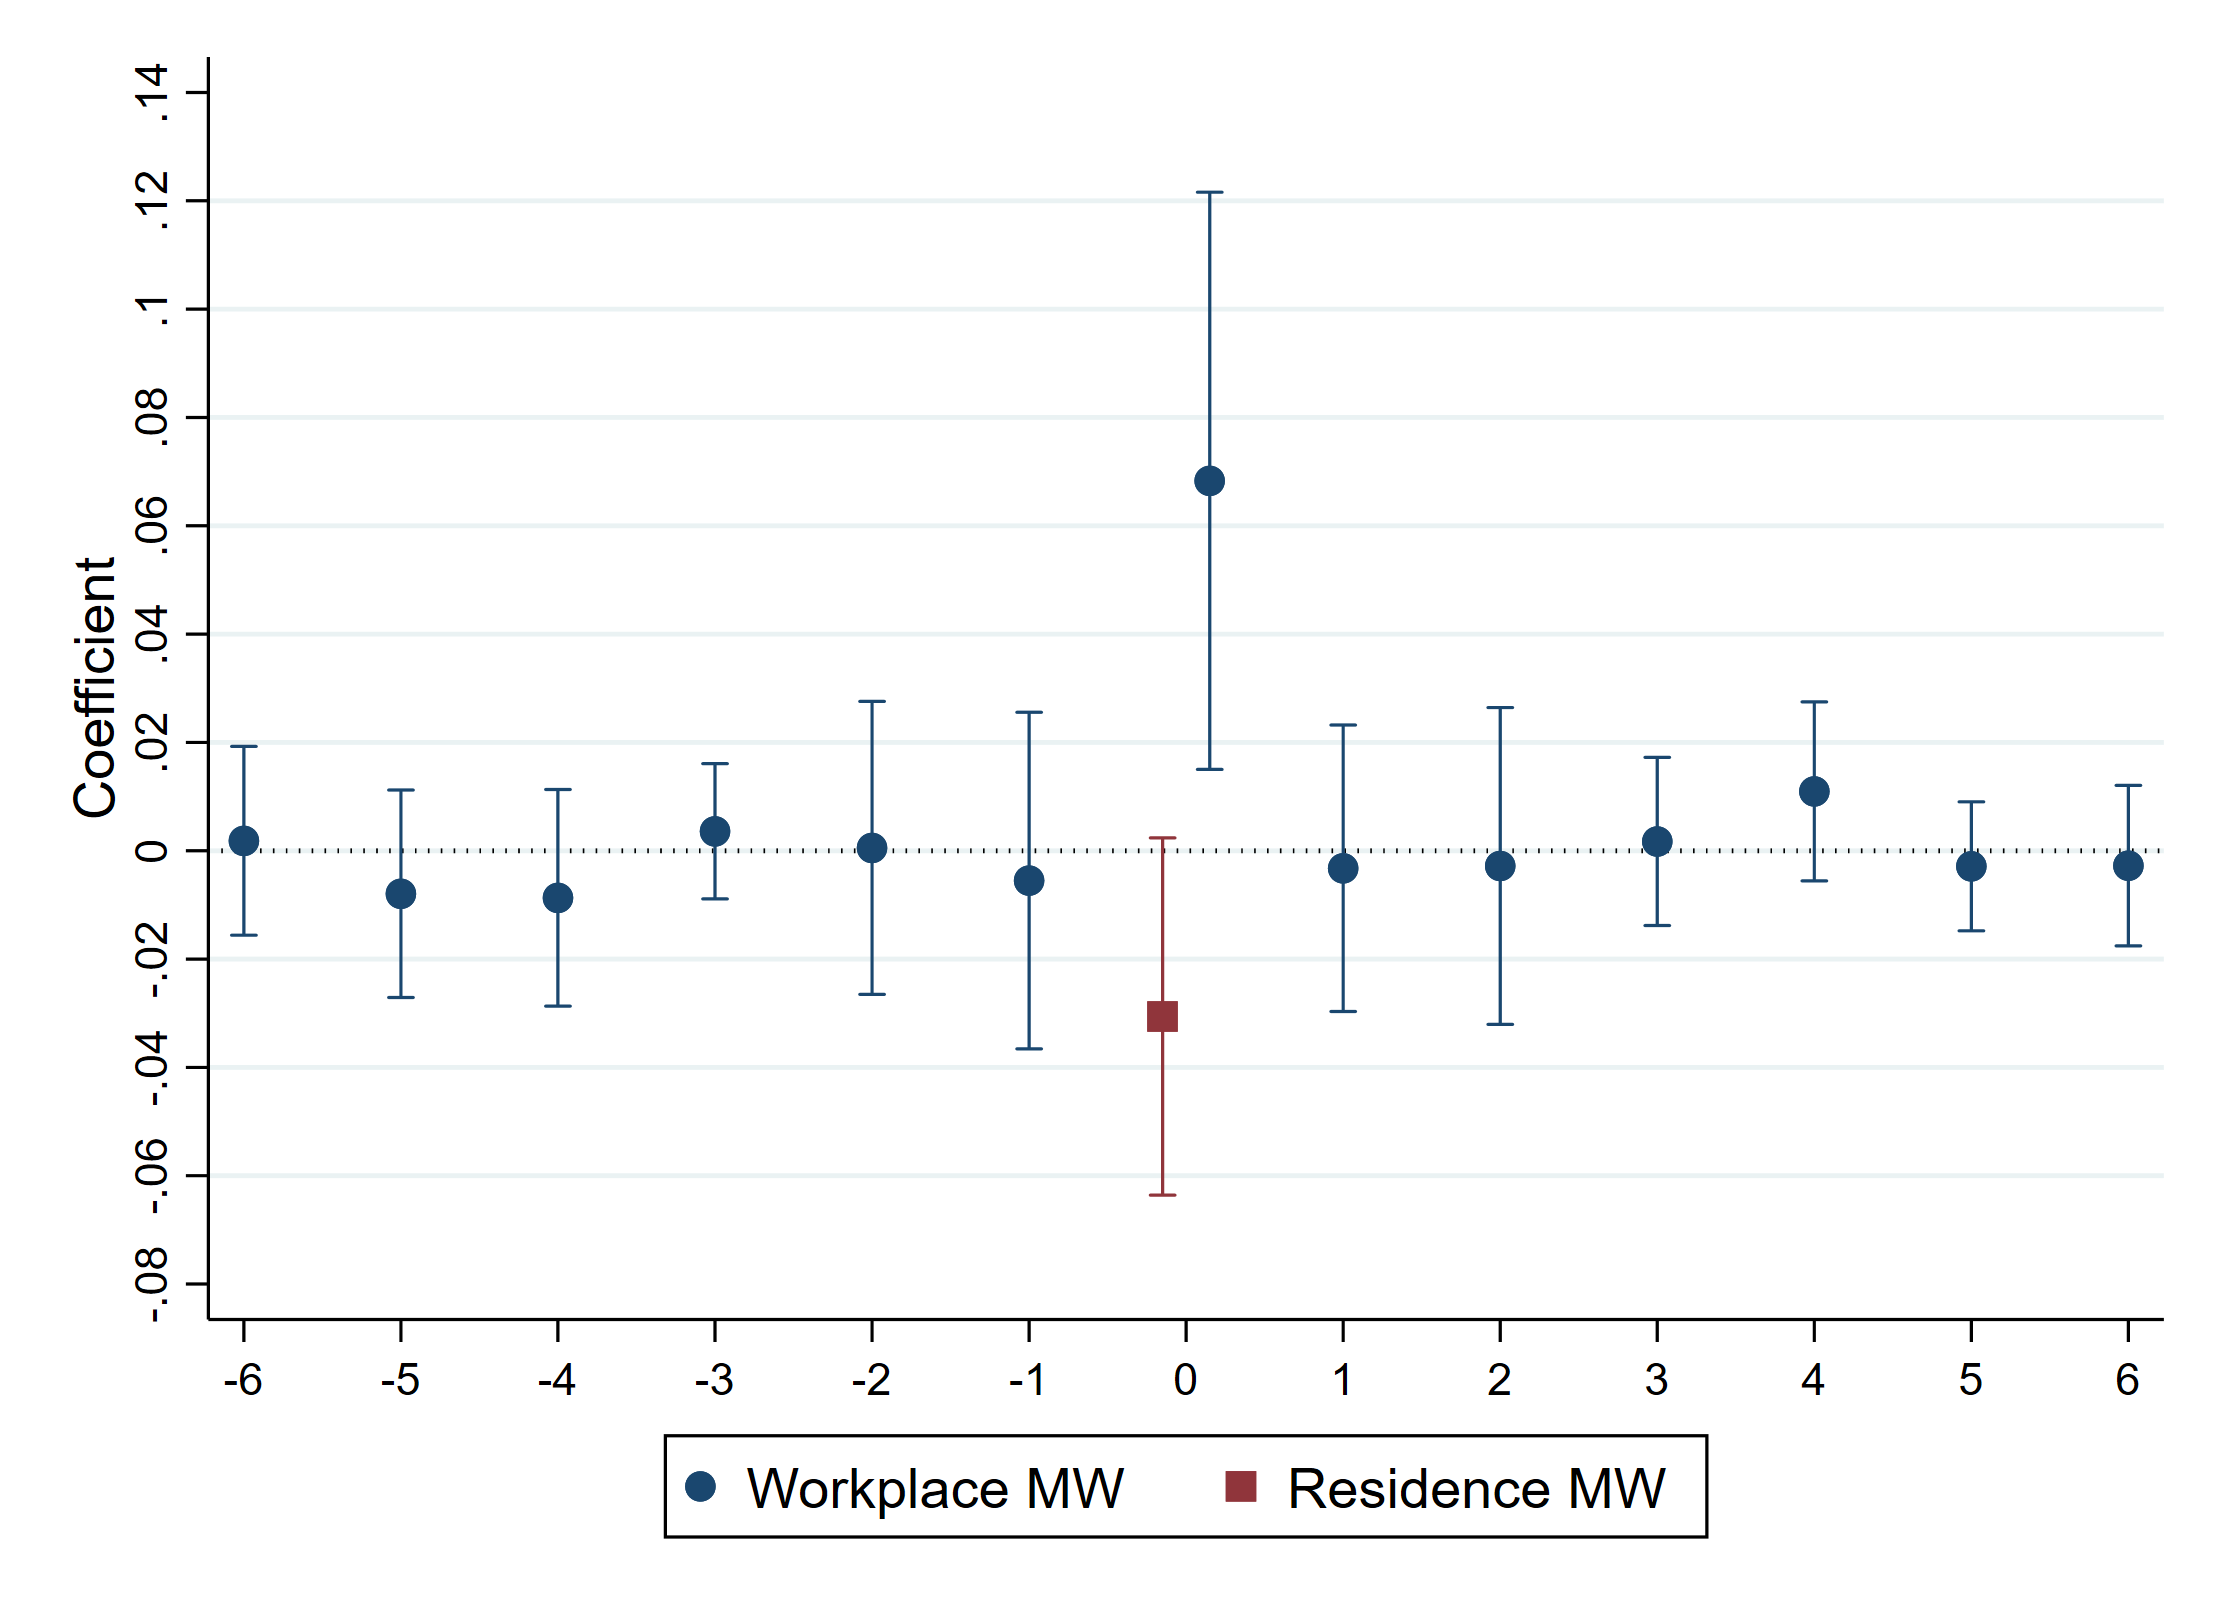
\includegraphics[width=0.68\textwidth]{fd_baseline/output/fd_both_mw_wkp_only_dynamic.png}
    \end{figure}
    
    \hyperlink{exclude_res}{\beamerbutton{Exclude residence MW}}
    \hyperlink{res_only_dyn}{\beamerbutton{Leads and lags of residence MW only}}
    \hyperlink{both_dyn}{\beamerbutton{Leads and lags of both}}
\end{frame}


\begin{frame}[label = robustness]
    \frametitle{Robustness checks and Sample Selection}

    Concerns about migration
    \begin{itemize}
        \item Literature finds small effects along several years {\small\color{gray}\parencite[e.g.,][]{PerezPerez2021}}
        \item Use different commuting shares, even allowing them to change yearly
        
        %\hyperlink{robustness_exp_mw}{\beamerbutton{Sensitivity to alternative commuting shares}}
    \end{itemize}

    \vspace{1.5mm}
    Concerns about parallel trends assumption
    \begin{itemize}
        \item Alternative strategies: ``stacked'' model and \textcite{ArellanoBond1991}
        \item Inclusion of non-parametric CBSA trends
        \item Inclusion of ZIP code-specific parametric trends
    \end{itemize}

    \vspace{1.5mm}
    Concerns that results are particular to our sample or not generalizable
    \begin{itemize}
        \item Estimate on unbalanced and fully-balanced samples (instead of partially balanced)
        \item Reweight observations to match characteristics of urban ZIP codes
        
        \hyperlink{robustness_sample}{\beamerbutton{Sample selection concerns}}
    \end{itemize}
    
\end{frame}

%%%%%%%%%%%%%%%%%%%%%%%%%%%%%%%%%%%%%%%%%%%%%%%%%%%%%%%%%%%%%%%%%%%%%%%%%%%%%%%%
\section{Counterfactual: A federal MW increase}

\begin{frame}
    \frametitle{Overview}
    
    Entire commuting structure determines the incidence of MW policies.
    \begin{itemize}
        \vspace{1mm}
        \item In some ZIP codes both residence and workplace MW increase
        \vspace{1mm}
        \item Other nearby ZIP codes are affected only through workplace
    \end{itemize}
    
    \pause
    \vspace{3mm}
    Consider an increase of the federal MW to \$9 in January 2020.
    \begin{itemize}
        \vspace{1mm}
        \item Changes income $\{\Delta Y_i\}_{i\in\Z}$ and housing expenditure $\{\Delta H_i\}_{i\in\Z}$
    \end{itemize}
    
    \pause
    \vspace{3mm}
    How much out of each extra dollar is captured by landlords?
   
\end{frame}

\begin{frame}
    \frametitle{Share pocketed by landlords}

    Define the share pocketed by landlords as 
    \begin{equation*}
        \rho_i := \frac{\Delta H_i}{\Delta Y_i} =  \frac{H^{\post}_i R^{\post}_i - H^{\pre}_i R^{\pre}_i}{\Delta Y_i}
    \end{equation*}
    where ``Pre'' and ``Post'' indicate moments before and after the increase.

    \pause
    \vspace{3mm}
    Change in rented space are unobserved. We assume $H^{\pre}_i = H^{\post}_i = H_i$ so
    \begin{equation*}
        \rho_i = \frac{H^{\post}_i R^{\post}_i - h^{\pre}_i R^{\pre}_i}{\Delta Y_i} = h_i \frac{\Delta R_i}{\Delta Y_i}
    \end{equation*}
    If $\Delta H_i > 0$ then our estimate of $\rho_i$ is a lower bound.

\end{frame}

\begin{frame}[label = share_pocketed_model]
    \frametitle{Share pocketed under the model}

    According to the model,
    $$
    \Delta r_i = \beta \Delta {\color{blue}\mw_i^{\wkp}} + \gamma {\color{red}\mw_i^{\res}}
    $$
    We also define, for $y_i = \ln Y_i$,
    $$
    \Delta y_i = \varepsilon \Delta {\color{blue}\mw_i^{\wkp}}
    $$
    We estimate $\varepsilon$ using IRS data. \hyperlink{wages_results}{\beamerbutton{Estimation results}}

    \pause
    \vspace{3mm}
    Algebra implies
    \begin{equation*}
        \rho_i = \alpha_i \left[
                  \frac{\exp \left( \beta \MW_i^{\text{wkr}} + \gamma \MW_i^{\text{res}} \right) - 1 }
                       {\exp \left( \varepsilon \MW_i^{\text{wkr}} \right) - 1 }
                         \right]
    \end{equation*}
    where $\alpha_i = \left(H_i R_i\right)/Y_i$ is the share of $i$'s expenditure in housing.

    \vspace{3mm}
    We use our estimates to compute $\rho_i$ for urban ZIP codes that are located
    in affected CBSAs.
\end{frame}

\begin{frame}
    \frametitle{Changes in residence and workplace MWs}

    \vspace{-2mm}
    
    \begin{figure}
        \begin{subfigure}{0.5\textwidth}
            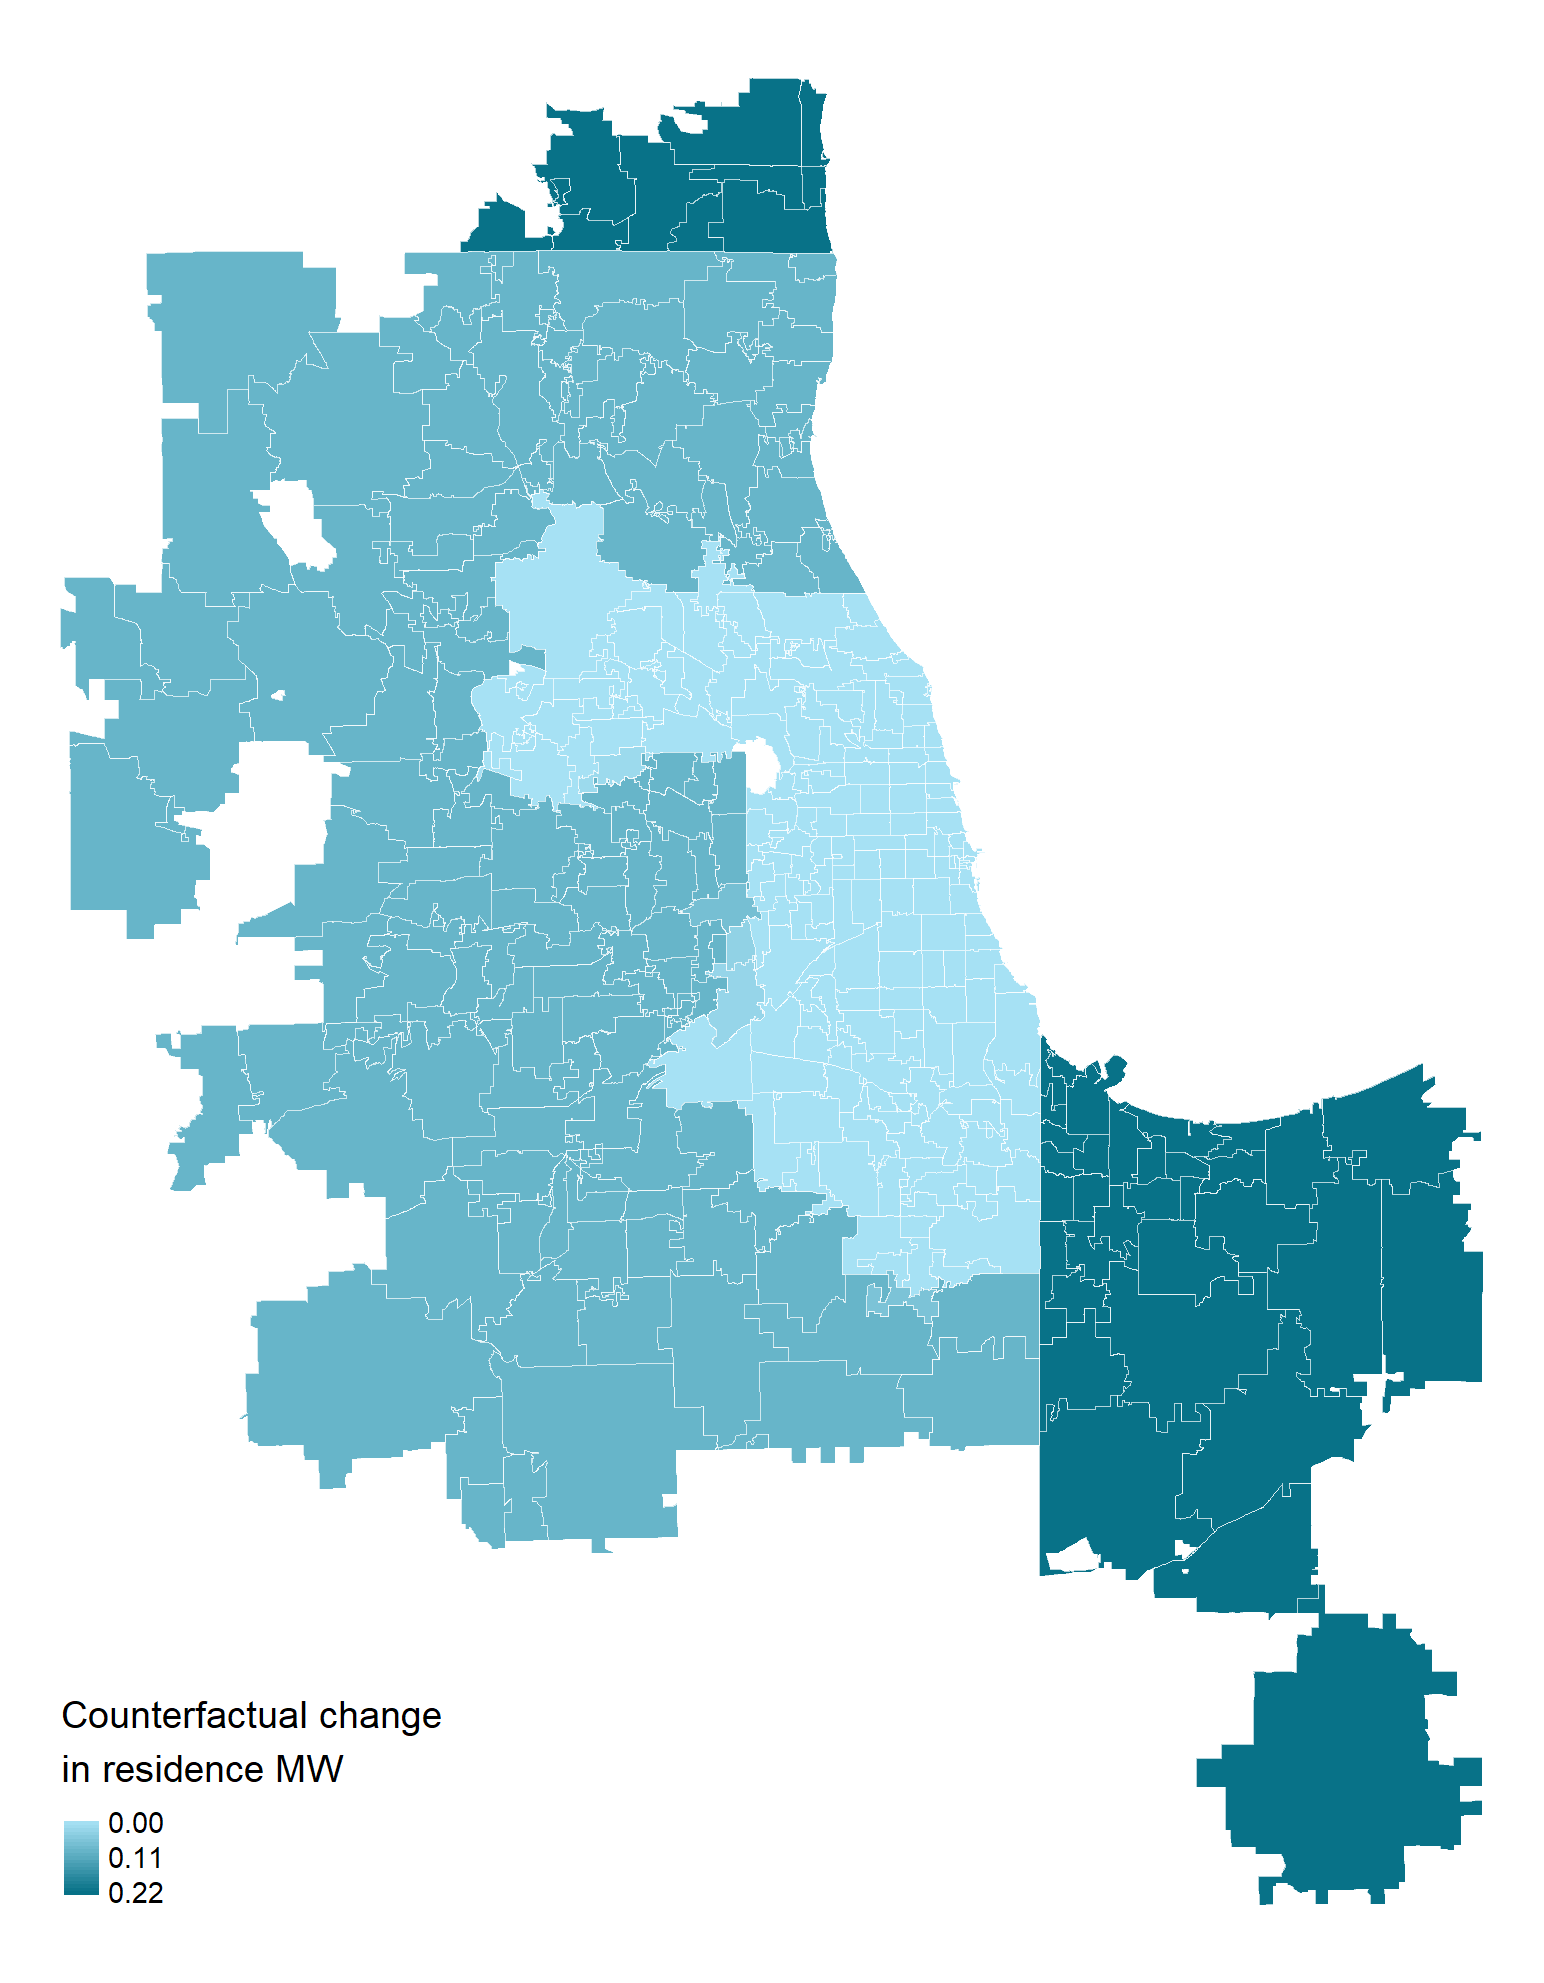
\includegraphics[width = 0.8\textwidth]{counterfactuals/output/chicago_d_mw_res.png}
            \caption*{Residence MW}
        \end{subfigure}%
        \begin{subfigure}{0.5\textwidth}
            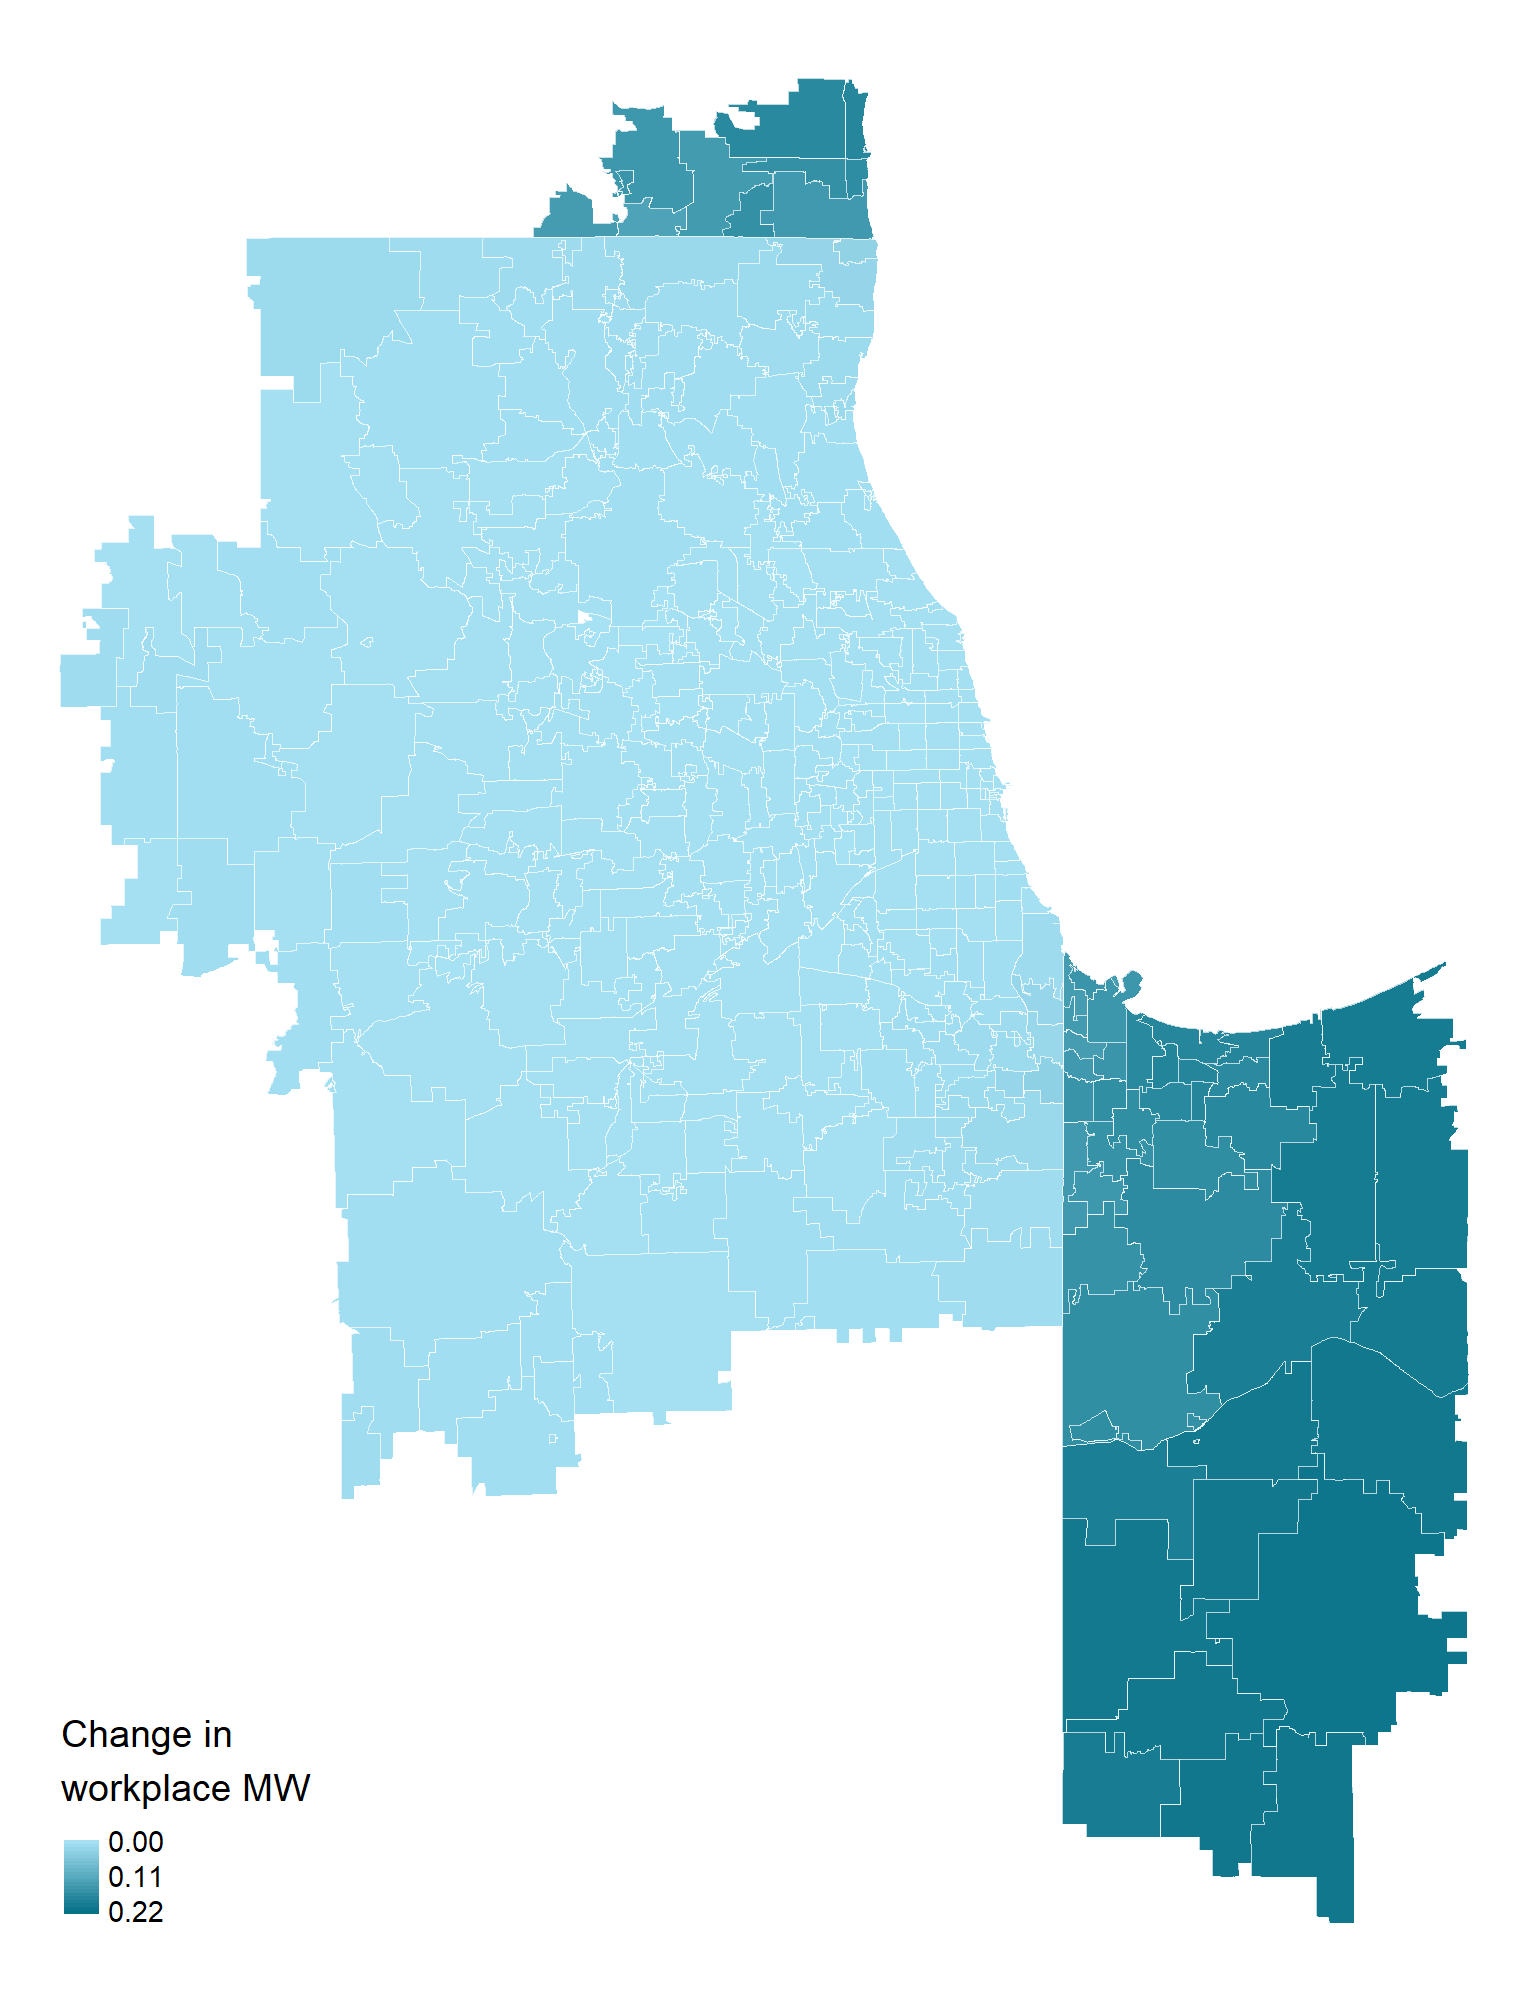
\includegraphics[width = 0.8\textwidth]{counterfactuals/output/chicago_d_mw_wkp.png}
            \caption*{Workplace MW}
        \end{subfigure}
    \end{figure}
\end{frame}

\begin{frame}
    \frametitle{Estimated changes in per-square-foot rents and total wages}

    \vspace{-2mm}

    \begin{figure}
        \begin{subfigure}{0.5\textwidth}
            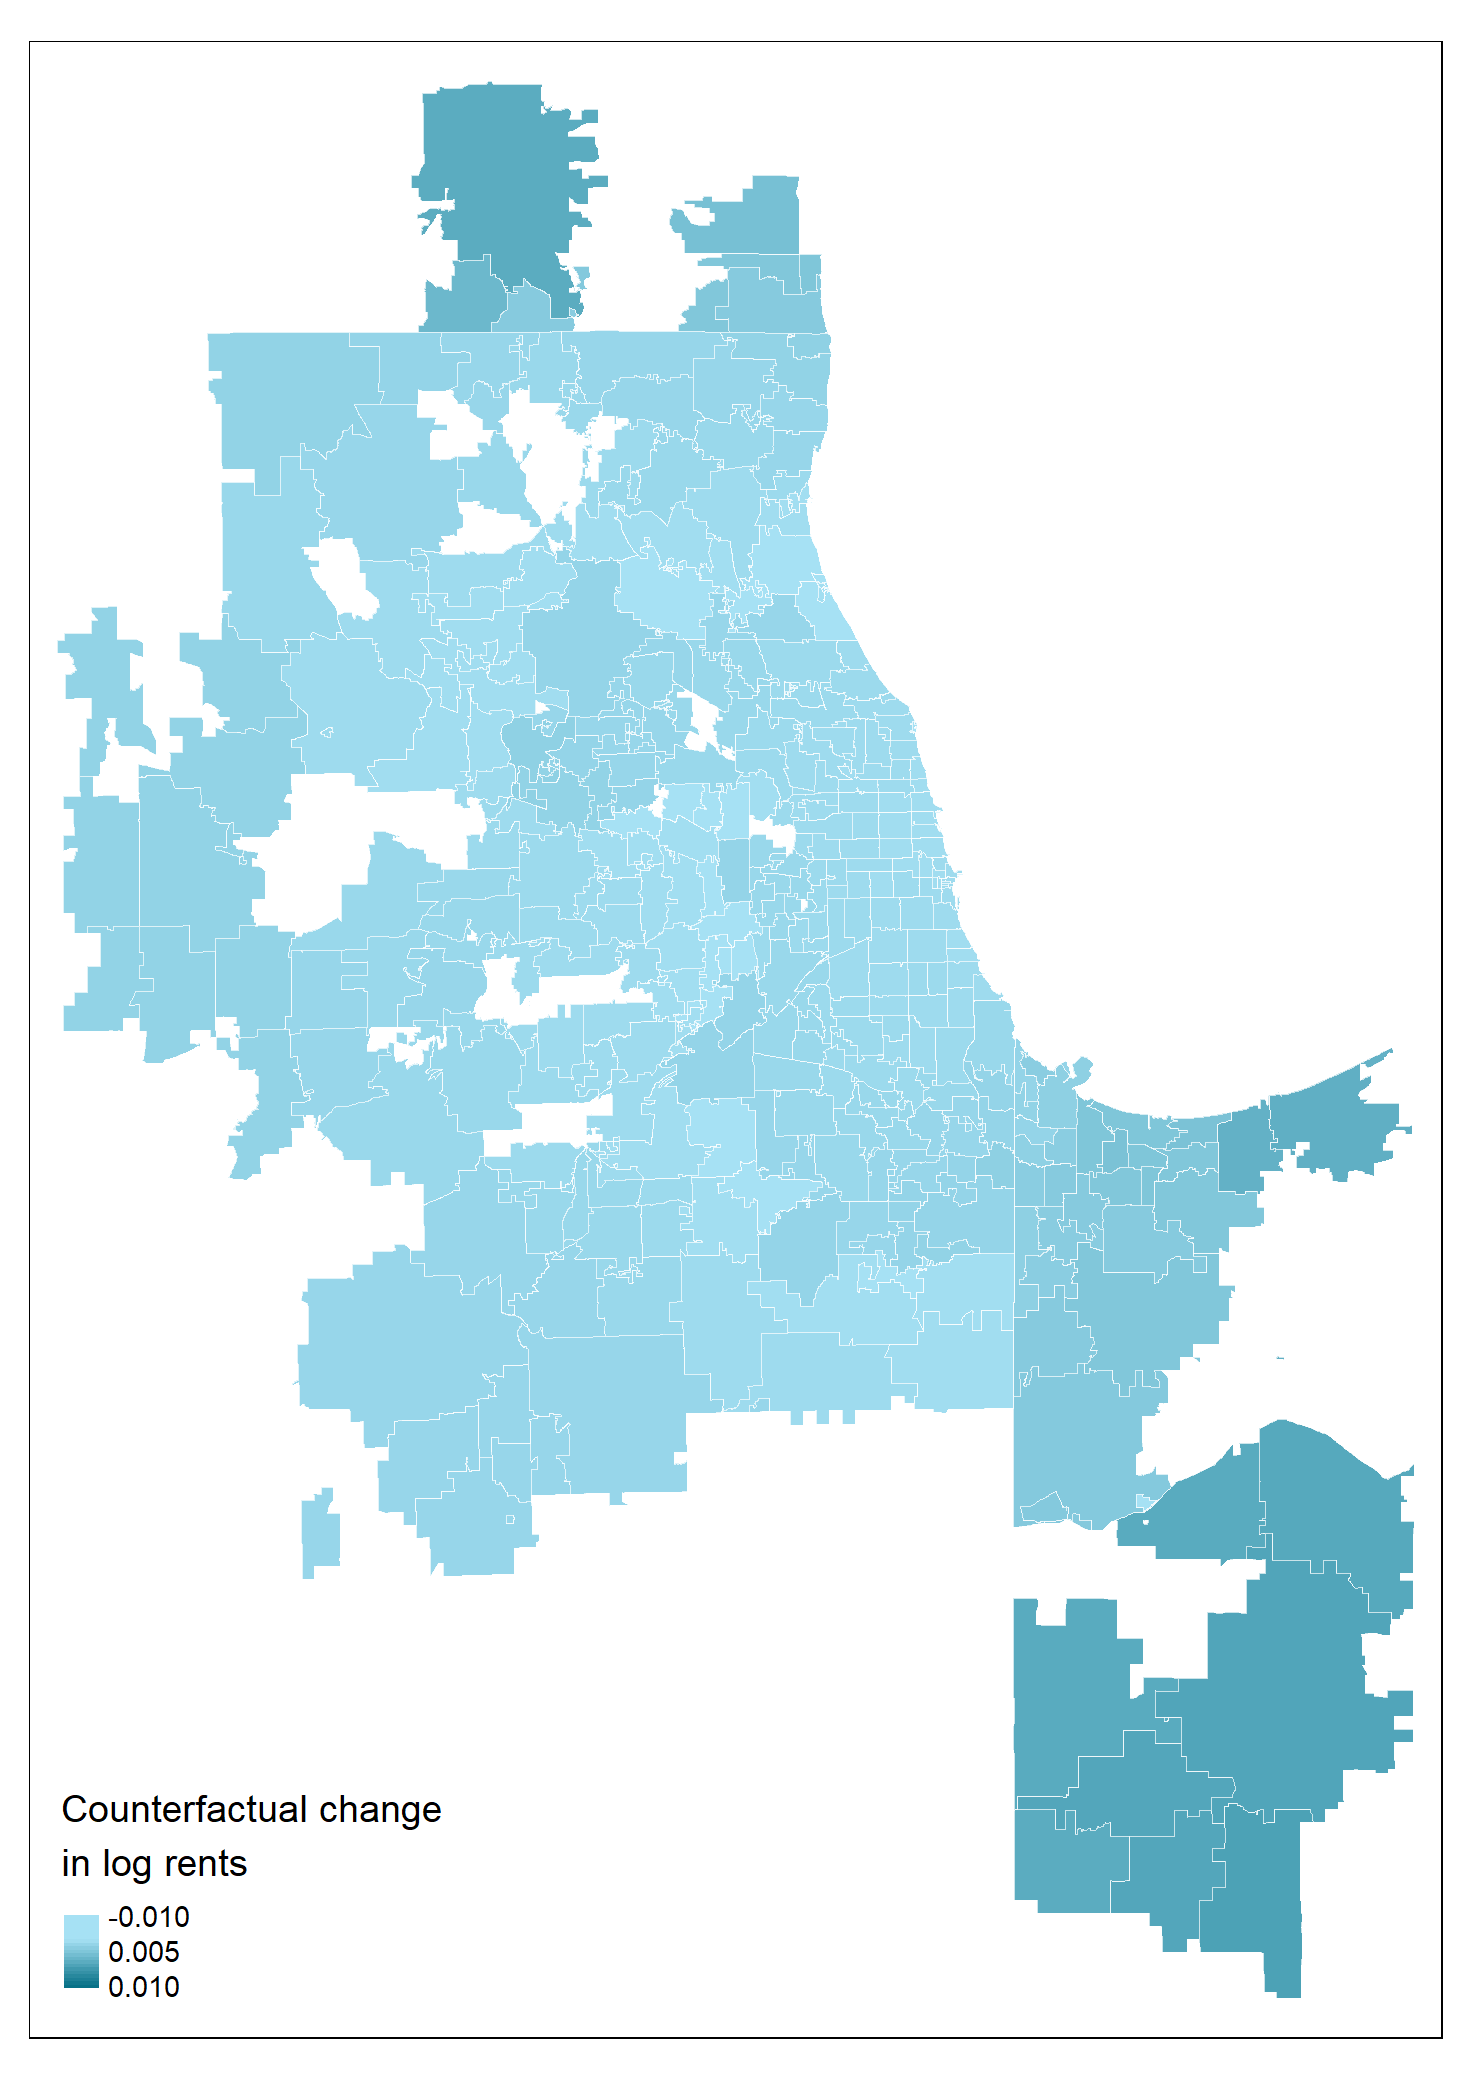
\includegraphics[width = 0.8\textwidth]{counterfactuals/output/chicago_d_ln_rents.png}
            \caption*{Changes in log rents per sqft.}
        \end{subfigure}%
        \begin{subfigure}{0.5\textwidth}
            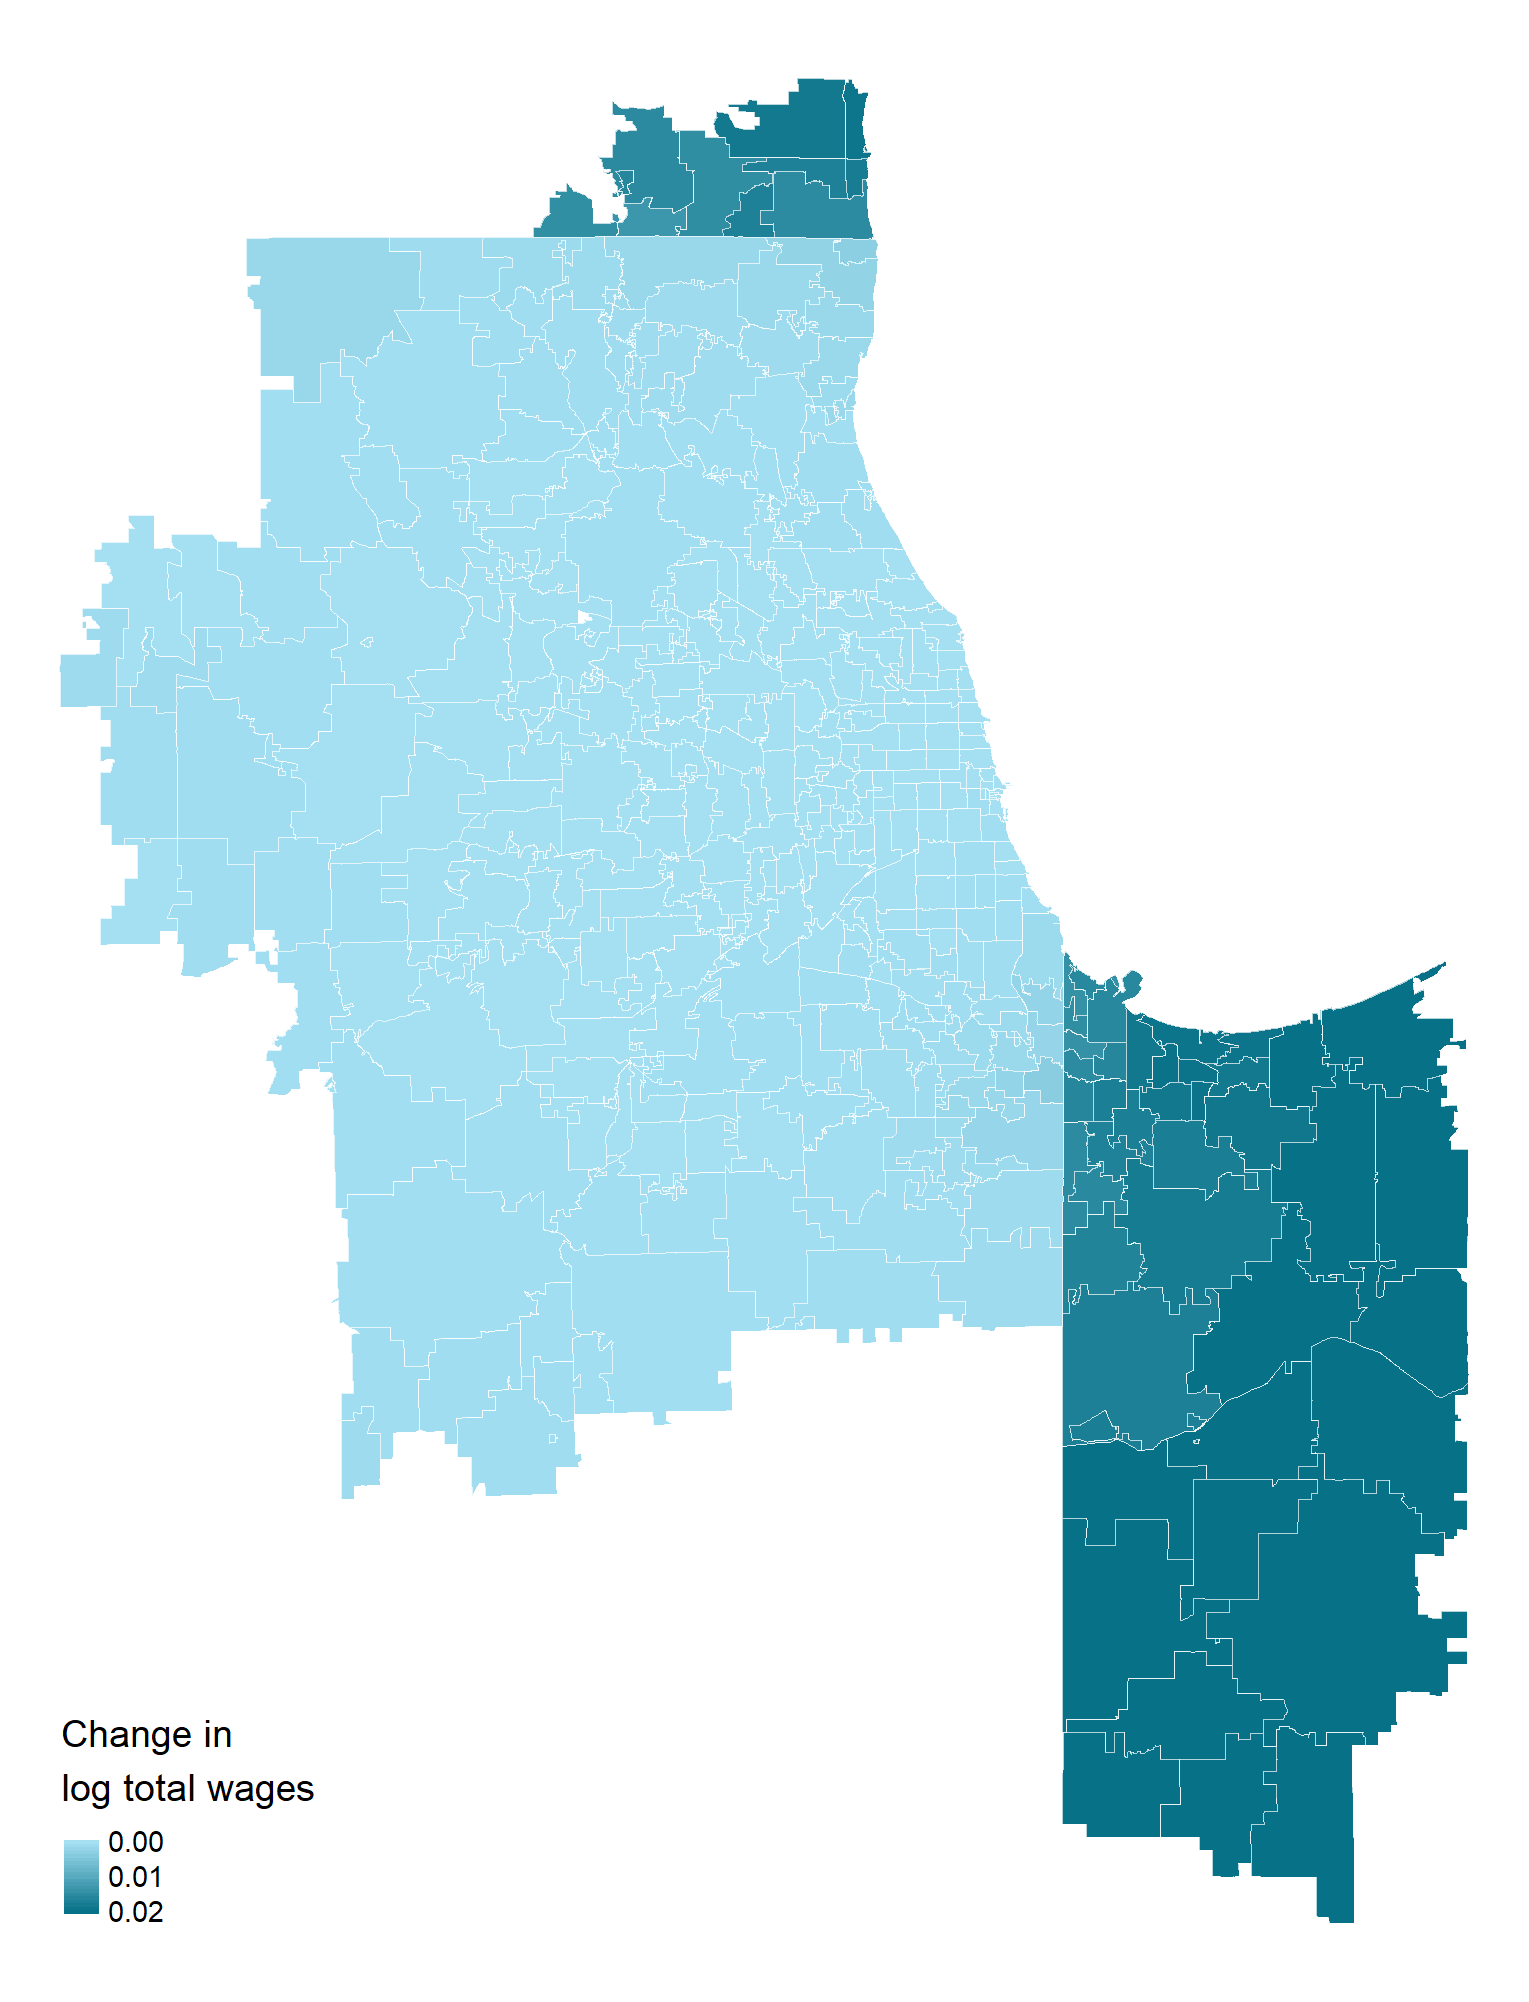
\includegraphics[width = 0.8\textwidth]{counterfactuals/output/chicago_d_ln_wagebill.png}
            \caption*{Changes in log total wages}
        \end{subfigure}
    \end{figure}
\end{frame}

\begin{frame}
    \frametitle{Share pocketed by landlords}

    \vspace{-3mm}

    \begin{figure}
        \centering
        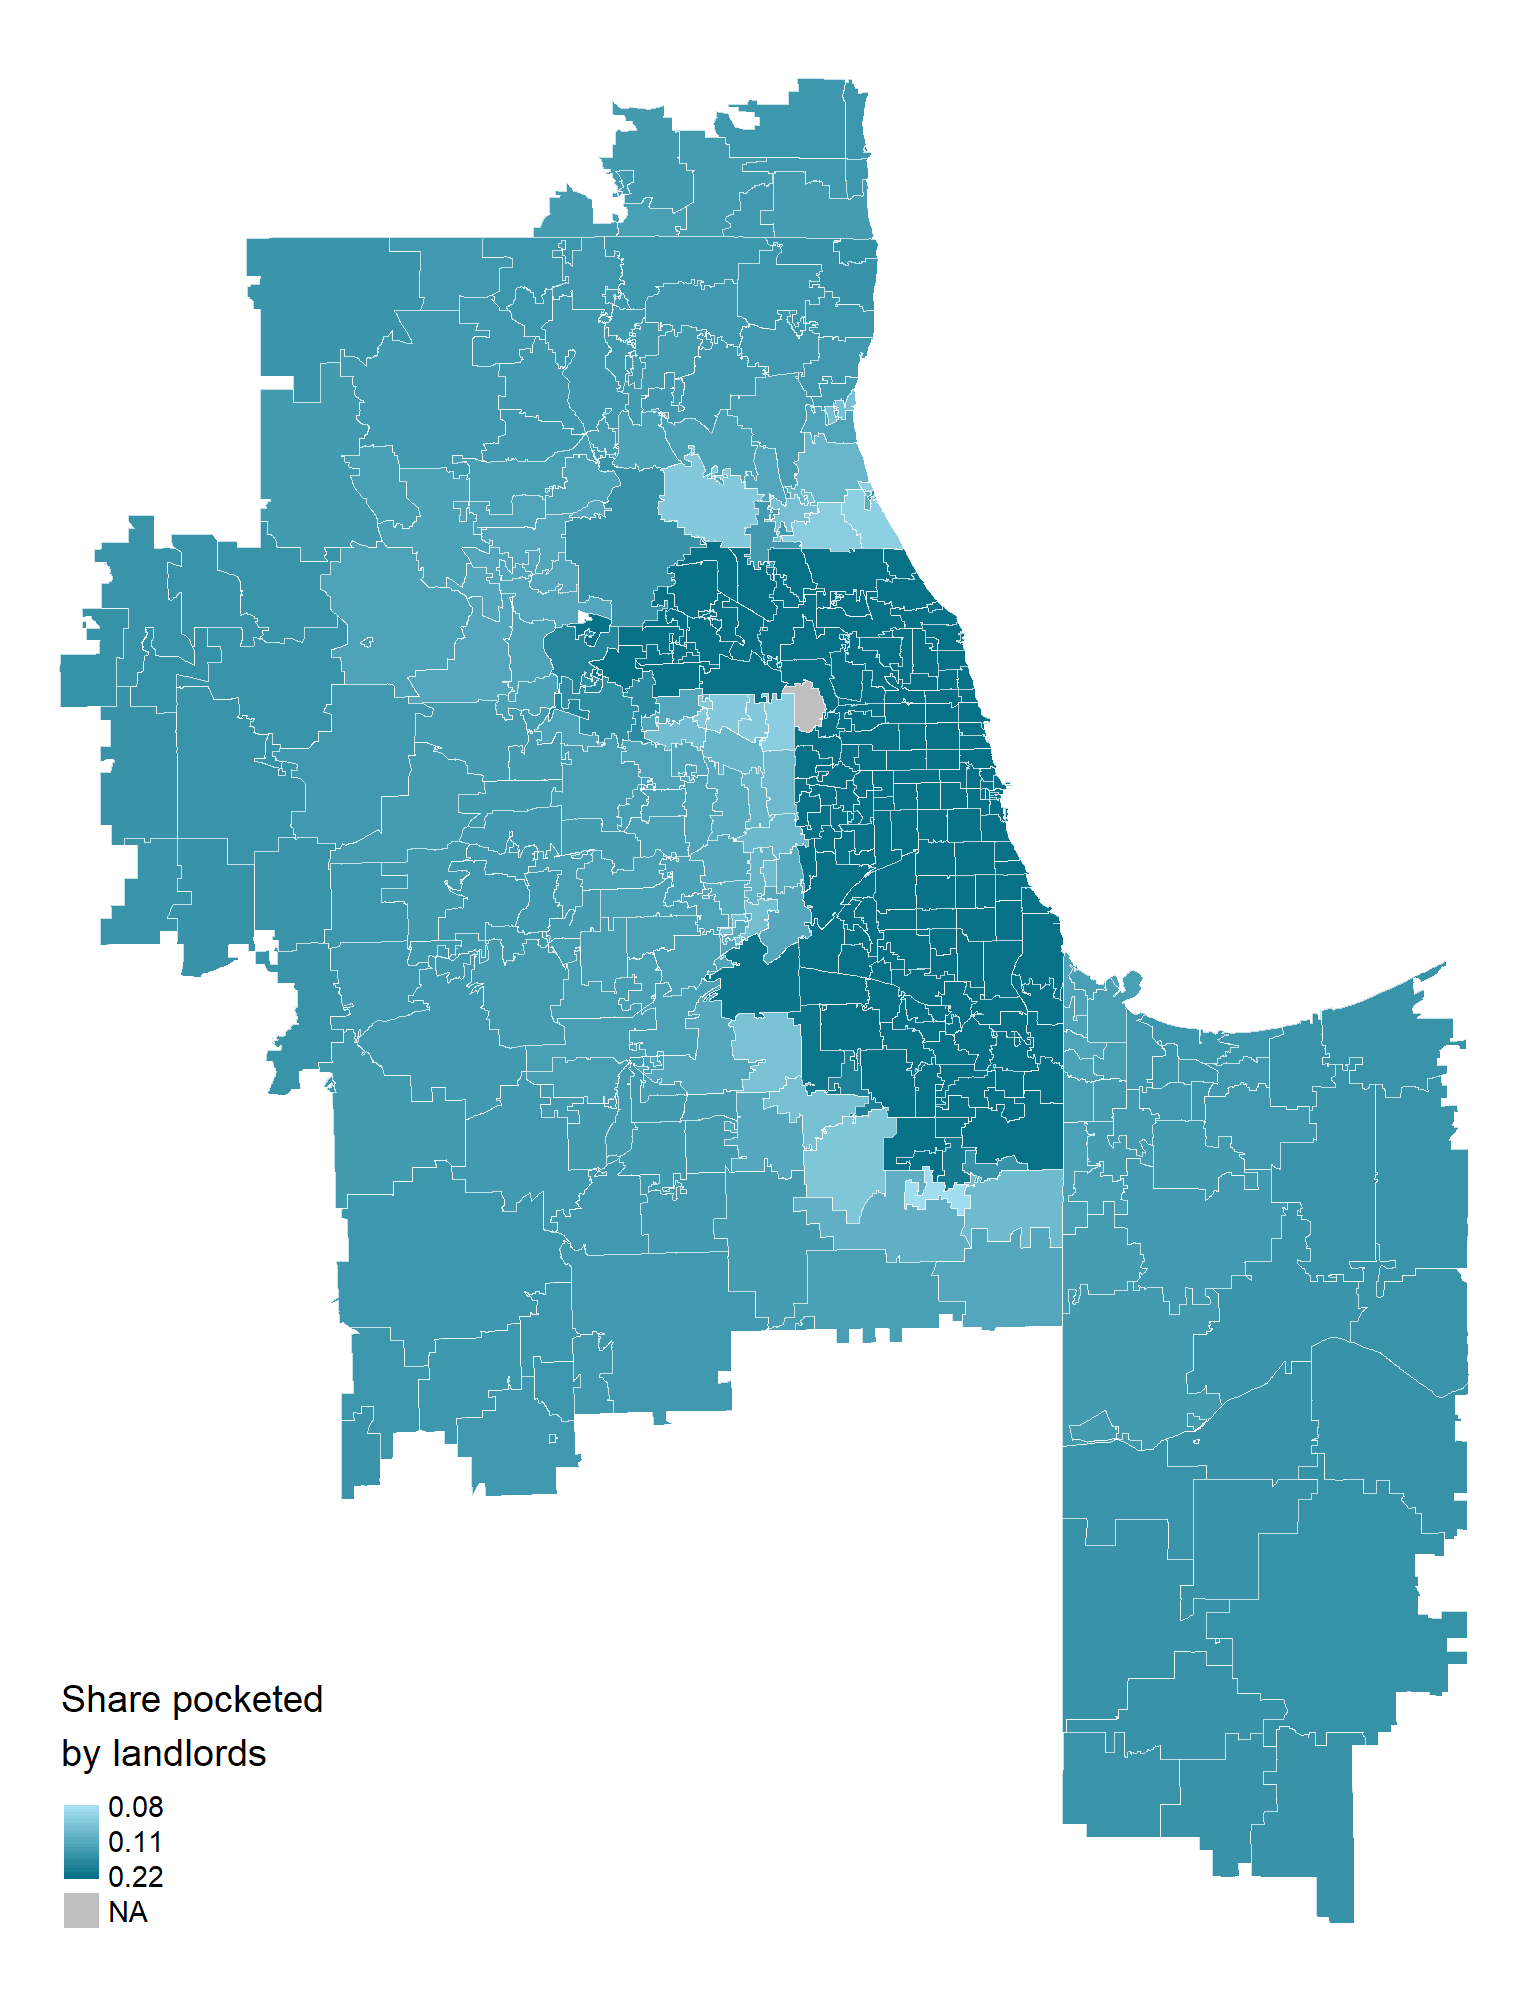
\includegraphics[width = 0.45\textwidth]{counterfactuals/output/chicago_rho.png}
    \end{figure}
\end{frame}

\begin{frame}
    \frametitle{The incidence of MW changes on average}
    
    \vspace{1mm}
    \begin{table}[hbt!]
    \centering
    \label{tab:counterfactuals_fed_9usd}

    \scalebox{0.85}{
    \begin{tabular}{@{}lccccc@{}}
        \toprule
                            &   & \multicolumn{2}{c}{Average change in...}
                                & \multicolumn{2}{c}{Avg.\ share pocketed}       \\ \cmidrule(lr){3-4}\cmidrule(lr){5-6}
                            & N & Res.\ MW & Wkp.\ MW
                            & $s = $ 0.25  & $s = $ 0.45                           \\ \midrule
        Effect in ZIP codes with...          &      &       &       &     &      \\
        $\quad$previous MW $\leq\$9\quad$    & 5,882 &  0.161 & 0.153  & 0.075 &  0.136   \\
        $\quad$previous MW $>\$9\quad$       & 1,070 &  0.000 & 0.017  & 0.126 & 0.227    \\ \bottomrule
    \end{tabular}
    }
\end{table}


    \pause
    \vspace{3mm}
    More generally, one can think of the effect for different values of 
    $$
        \Delta \mw_i^{\wkp} - \Delta \mw_i^{\res}
    $$
\end{frame}

\begin{frame}
    \frametitle{The incidence of MW changes according to intensity of treatment}
    
    \begin{figure}
        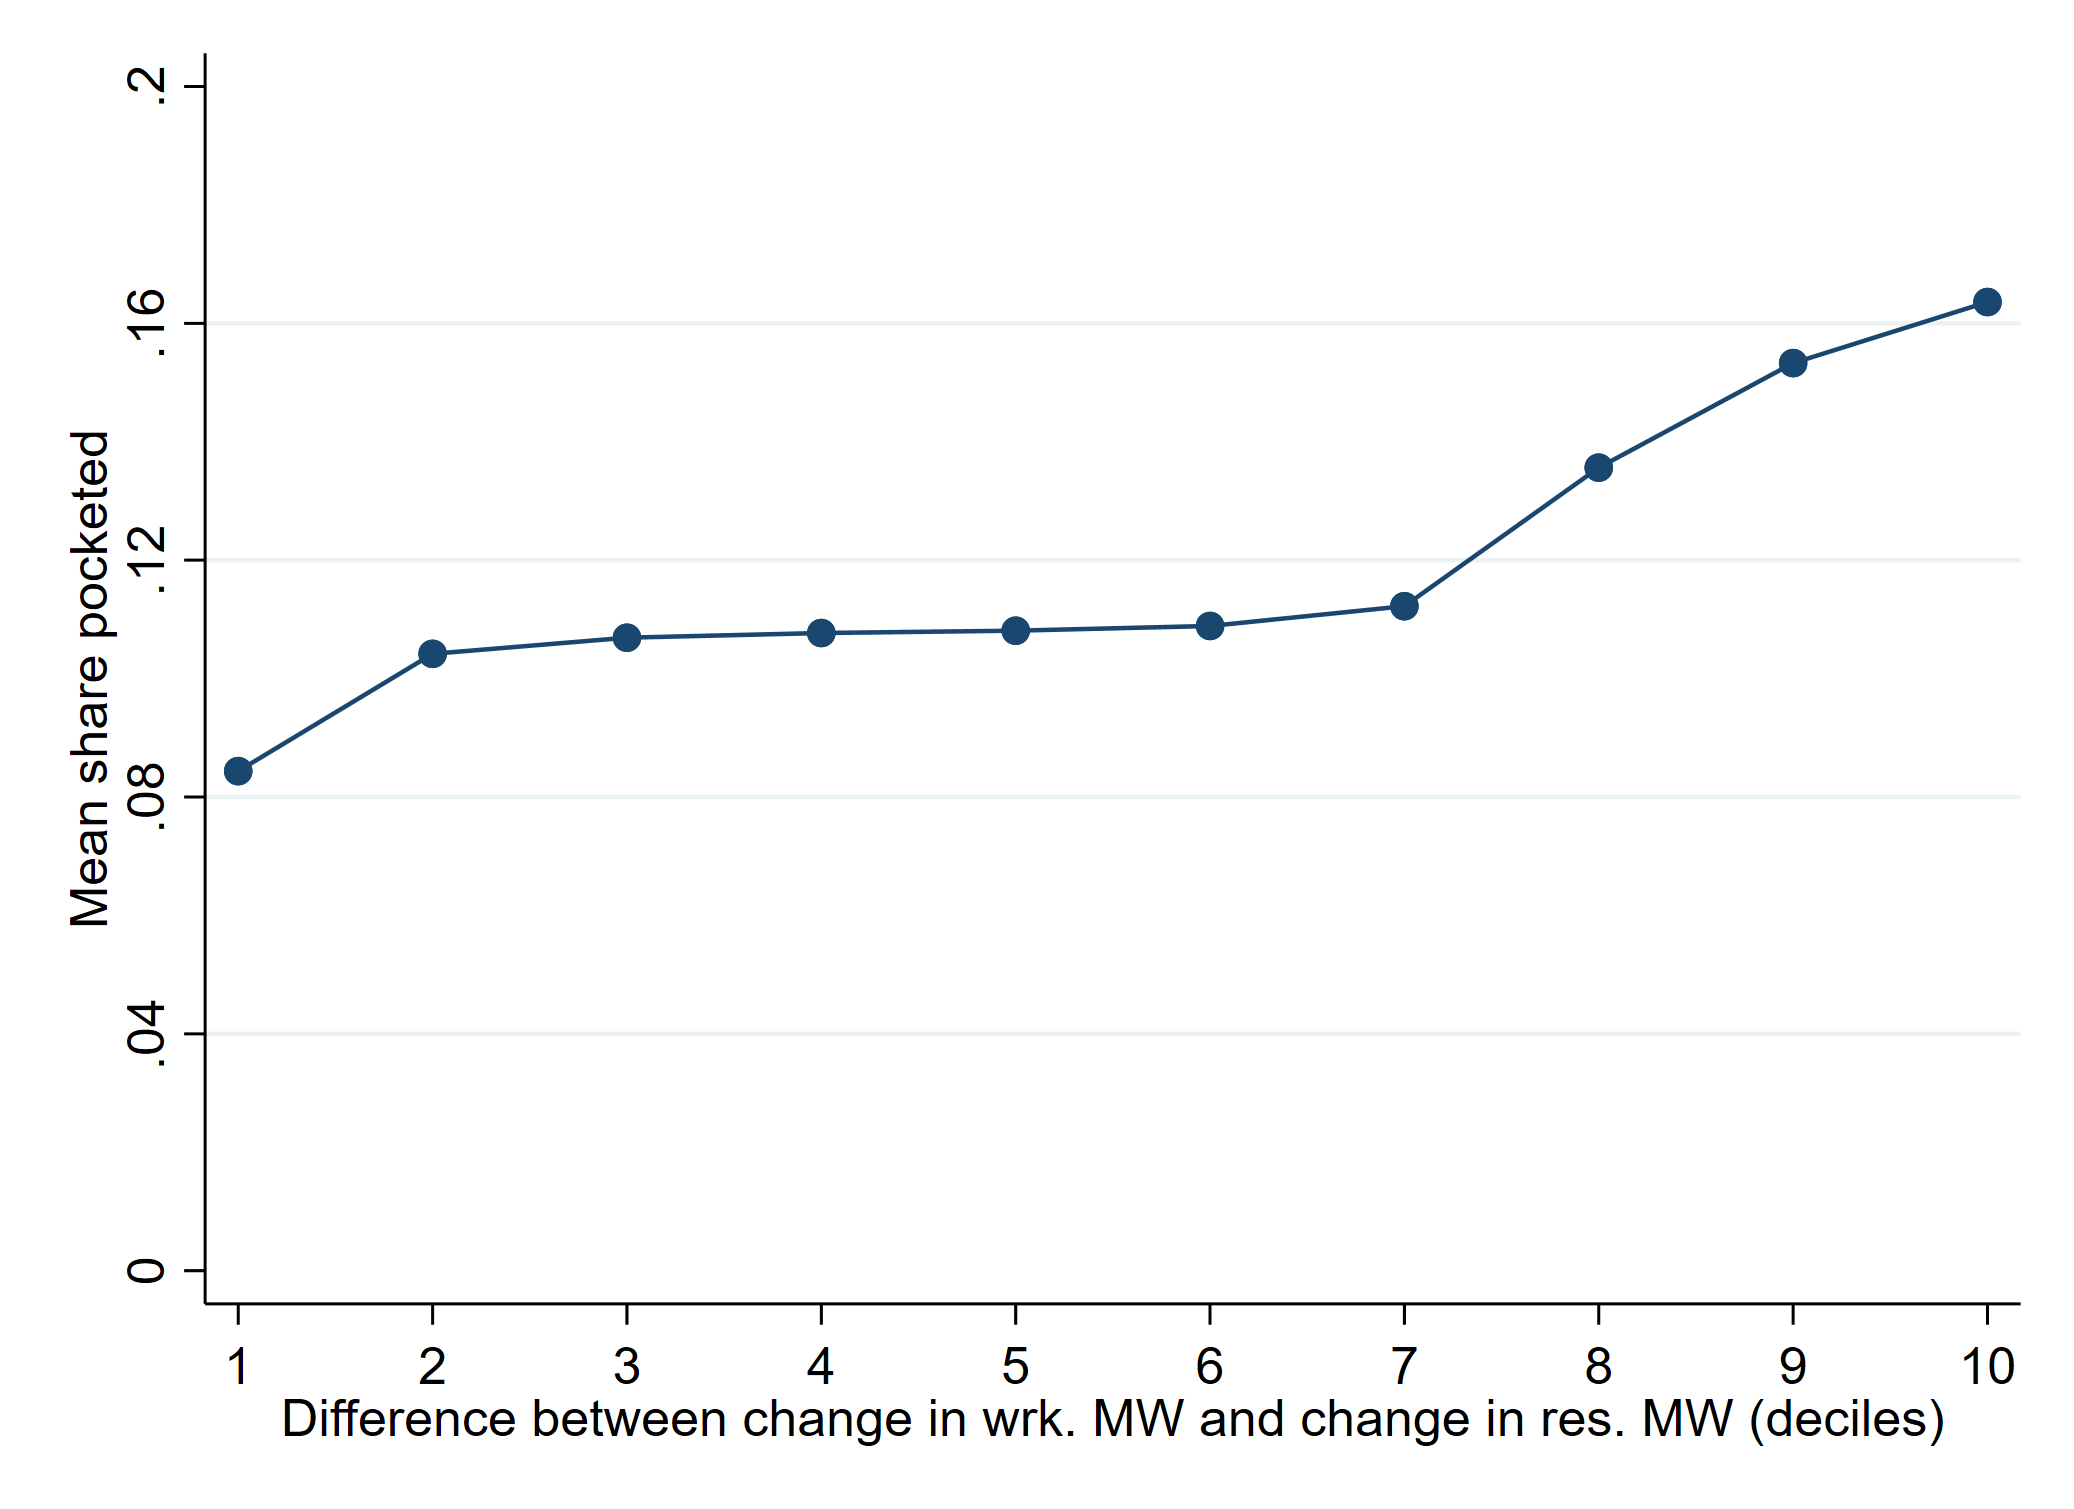
\includegraphics[width = 0.63\textwidth]{counterfactuals/output/deciles_diff.png}
    \end{figure}
    \vspace{.5mm}
    \footnotesize
    Notes: The figure shows computations of the share pocketed for the following
    parameters: $\beta = 0.0546$, $\gamma = -0.0207$, $\varepsilon = 0.1083$, and $\alpha=0.35$.
\end{frame}

%%%%%%%%%%%%%%%%%%%%%%%%%%%%%%%%%%%%%%%%%%%%%%%%%%%%%%%%%%%%%%%%%%%%%%%%%%%%%%%%
\section{Concluding remarks}

\begin{frame}
    \frametitle{Conclusion}
    
    \begin{itemize}
        \item When studying effects of place-based policies on housing market must account for 
        divergence between workplace and residence locations
         \vspace{2mm}
         \item In the case of the MW, hikes in workplace locations \textit{increase} rents
         whereas hikes in residence locations \textit{decrease} rents
         \vspace{2mm}
         \item Even with a two-parameter model we are able to describe and predict rich spatial patterns in rent changes
         \vspace{2mm}
         \item Landlords pocket a non-negligible fraction of the income increase generated by the MW
    \end{itemize}
    
\end{frame}

\begin{frame}[c]
    \Large Thank You!

    \vspace{3mm}
    \normalsize E-mail: \texttt{\url{santiago_hermo@brown.edu}}
\end{frame}

%%%%%%%%%%%%%%%%%%%%%%%%%%%%%%%%%%%%%%%%%%%%%%%%%%%%%%%%%%%%%%%%%%%%%%%%%%%%%%%%%%%%%%%%%%
%                                       APPENDIX                                        %
%%%%%%%%%%%%%%%%%%%%%%%%%%%%%%%%%%%%%%%%%%%%%%%%%%%%%%%%%%%%%%%%%%%%%%%%%%%%%%%%%%%%%%%%%%

\appendix

\renewcommand\thetable{\thesection.\arabic{table}}
\renewcommand\thefigure{\thesection.\arabic{figure}} 
\setcounter{table}{0}
\setcounter{figure}{0}

\section{Appendix}

\begin{frame}[label = nyc_example]
\frametitle{New York (MW changes in January 2019)}
    \begin{columns}
        \begin{column}{0.50\textwidth}
            \vspace{-4mm}
            \begin{figure}
                \centering
                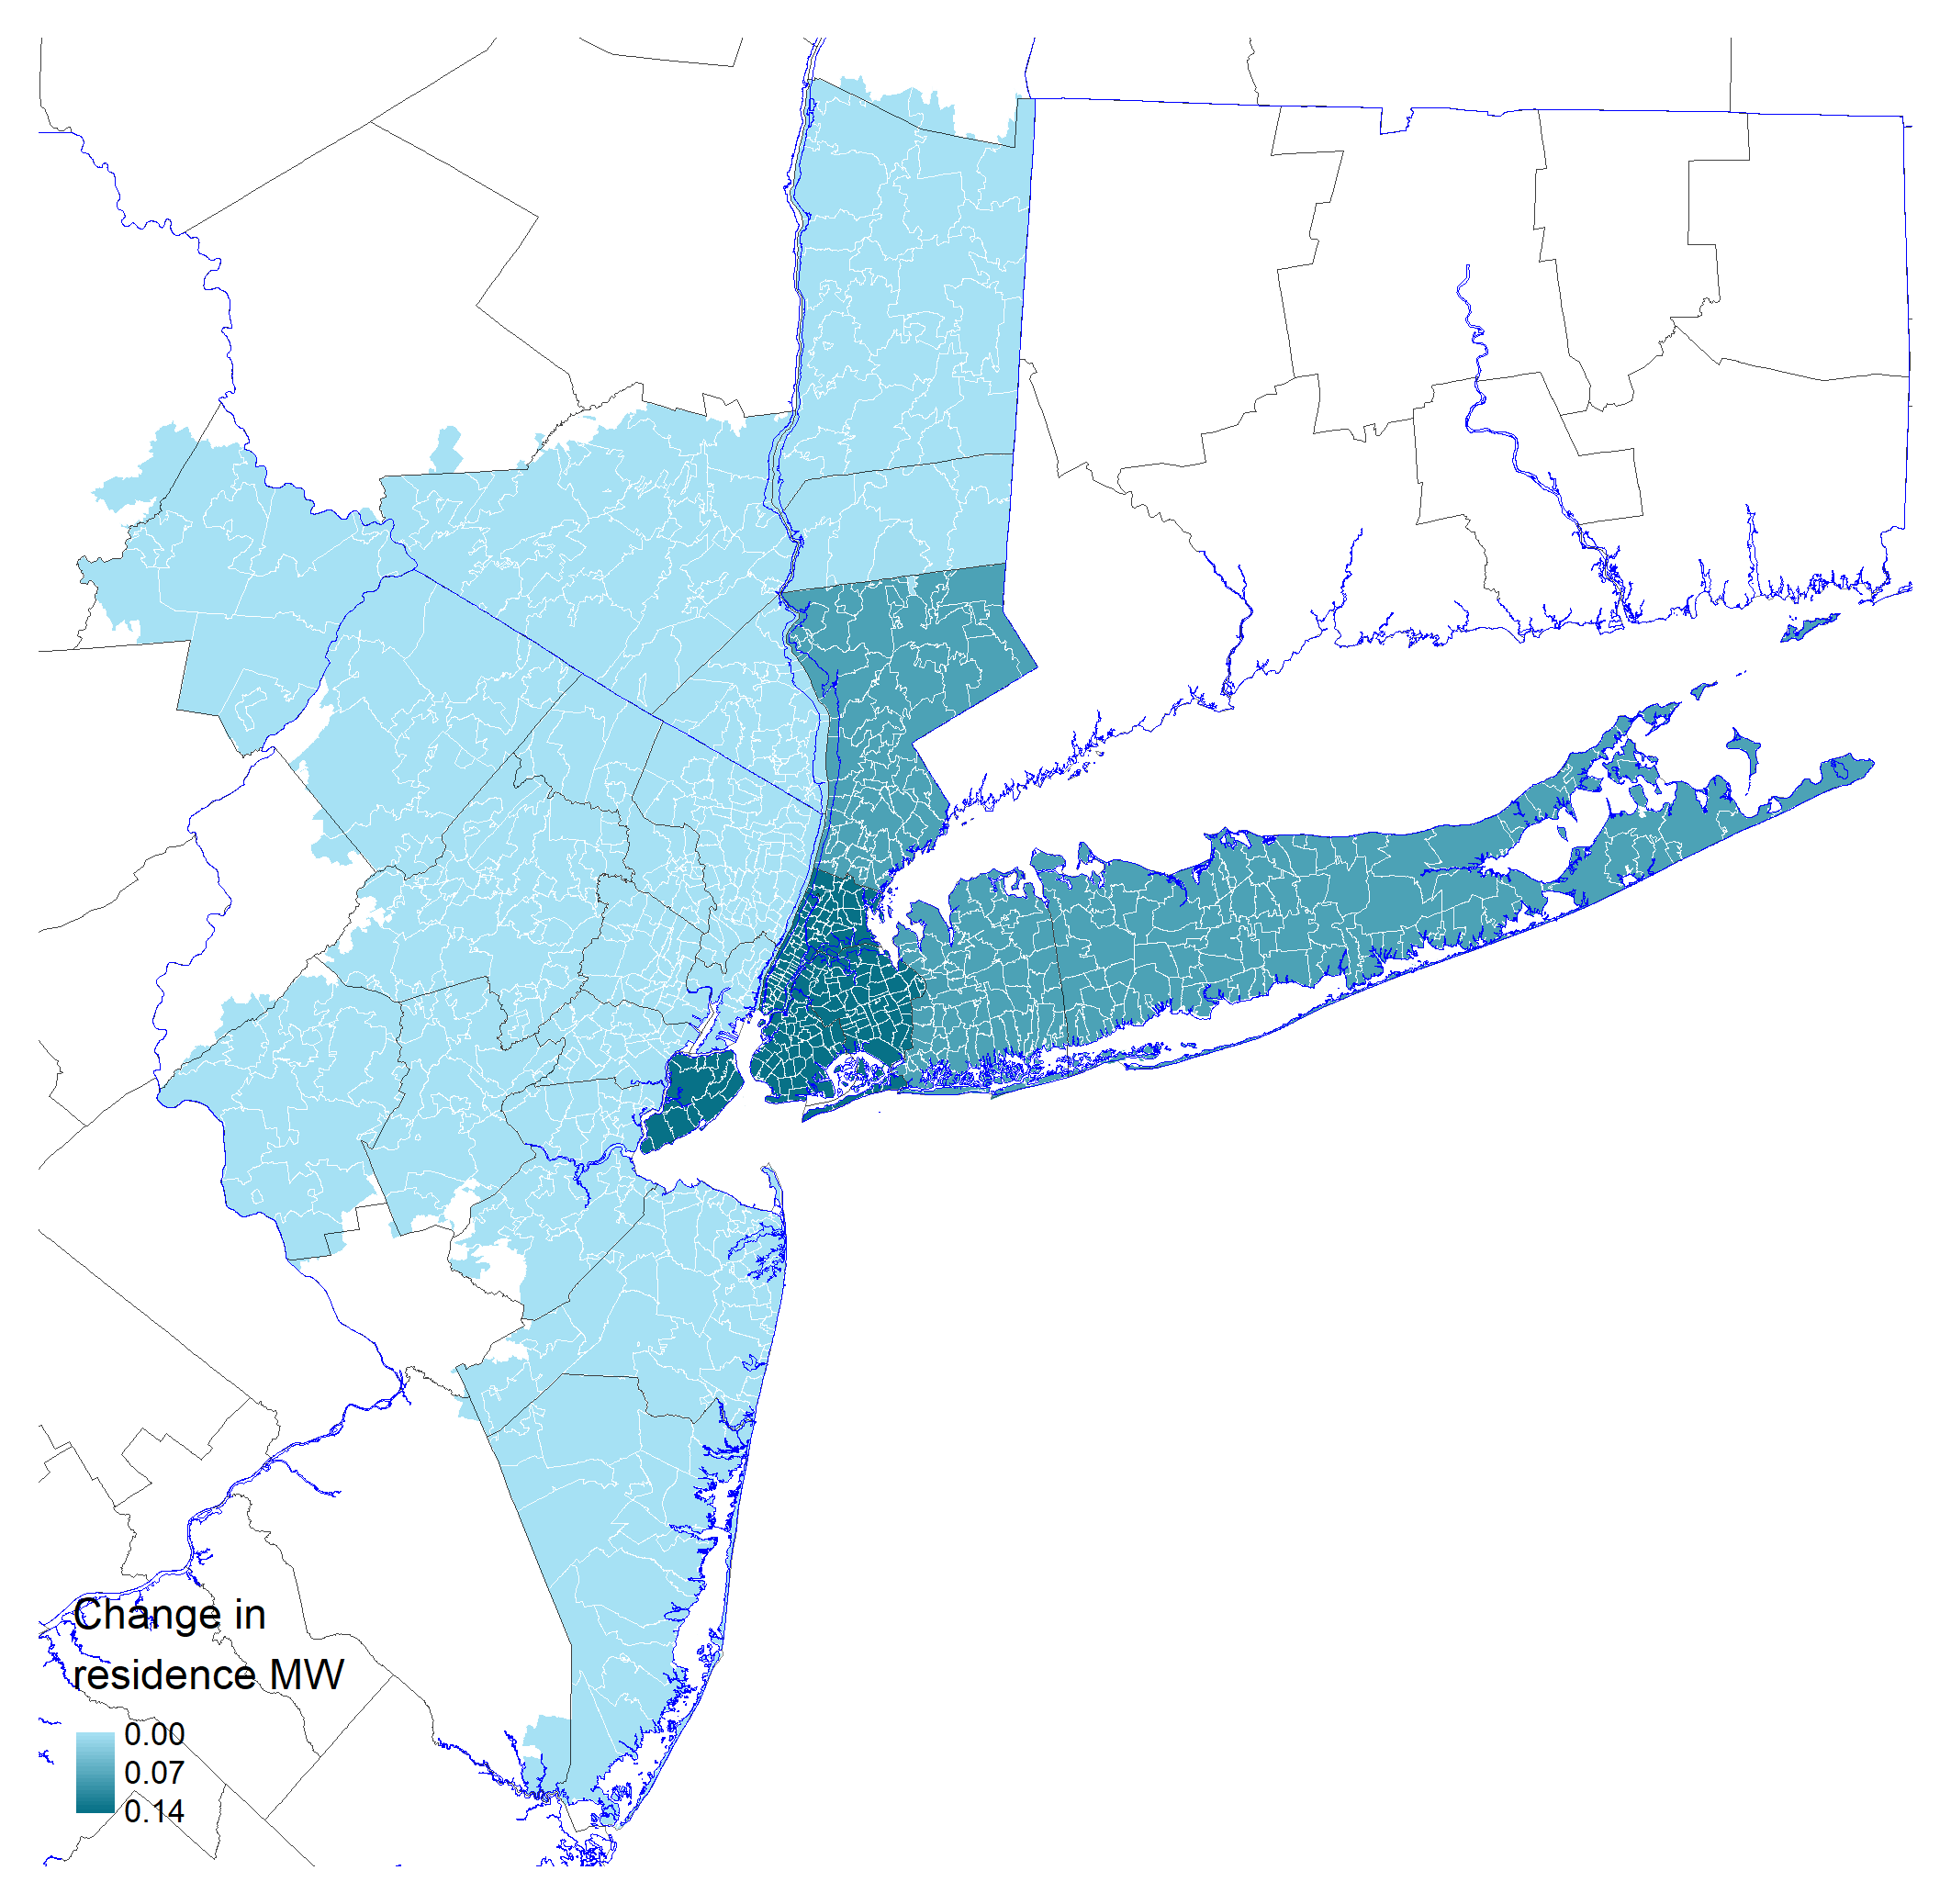
\includegraphics[scale = 0.36]{maps_events/output/nyc_2018-12_statutory_mw.png}
            \end{figure}   
        \end{column}
        \begin{column}{0.50\textwidth}
            \vspace{-4mm}
            \begin{figure}
                \centering
                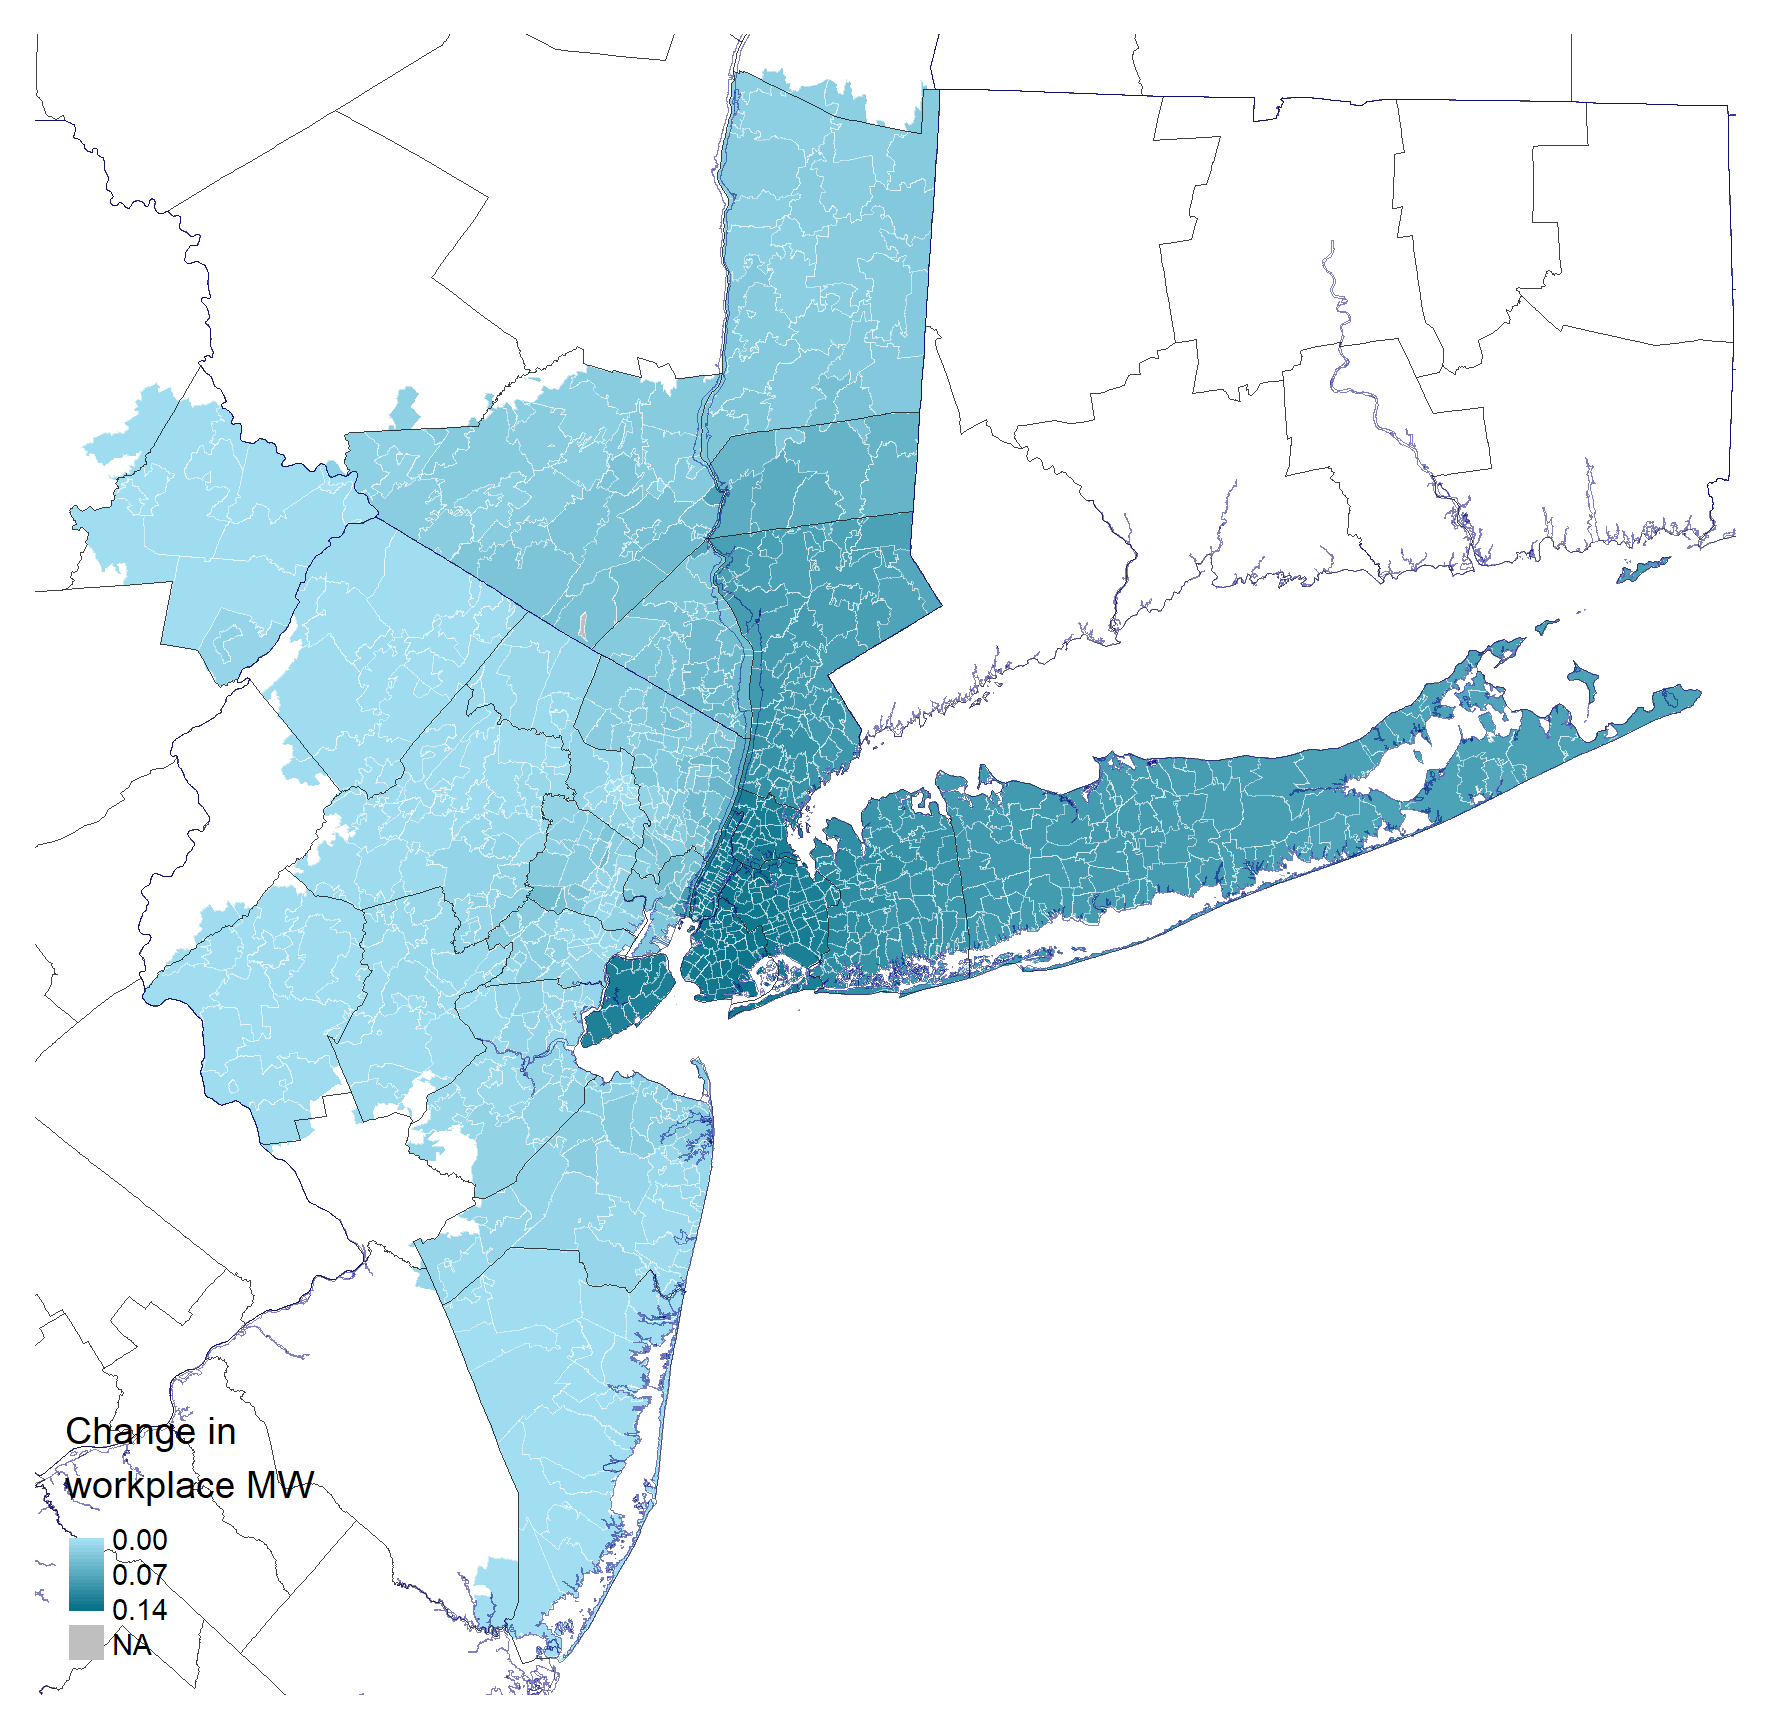
\includegraphics[scale = 0.36]{maps_events/output/nyc2018-12_wkp_mw.png}
            \end{figure}   
        \end{column}
    \end{columns}
    \hyperlink{chi_example}{\beamerbutton{Go back}}
\end{frame}

\begin{frame}[label = bay_example]
\frametitle{Bay area (MW changes in January 2019)}
    \begin{columns}
        \begin{column}{0.50\textwidth}
            \vspace{-4mm}
            \begin{figure}
                \centering
                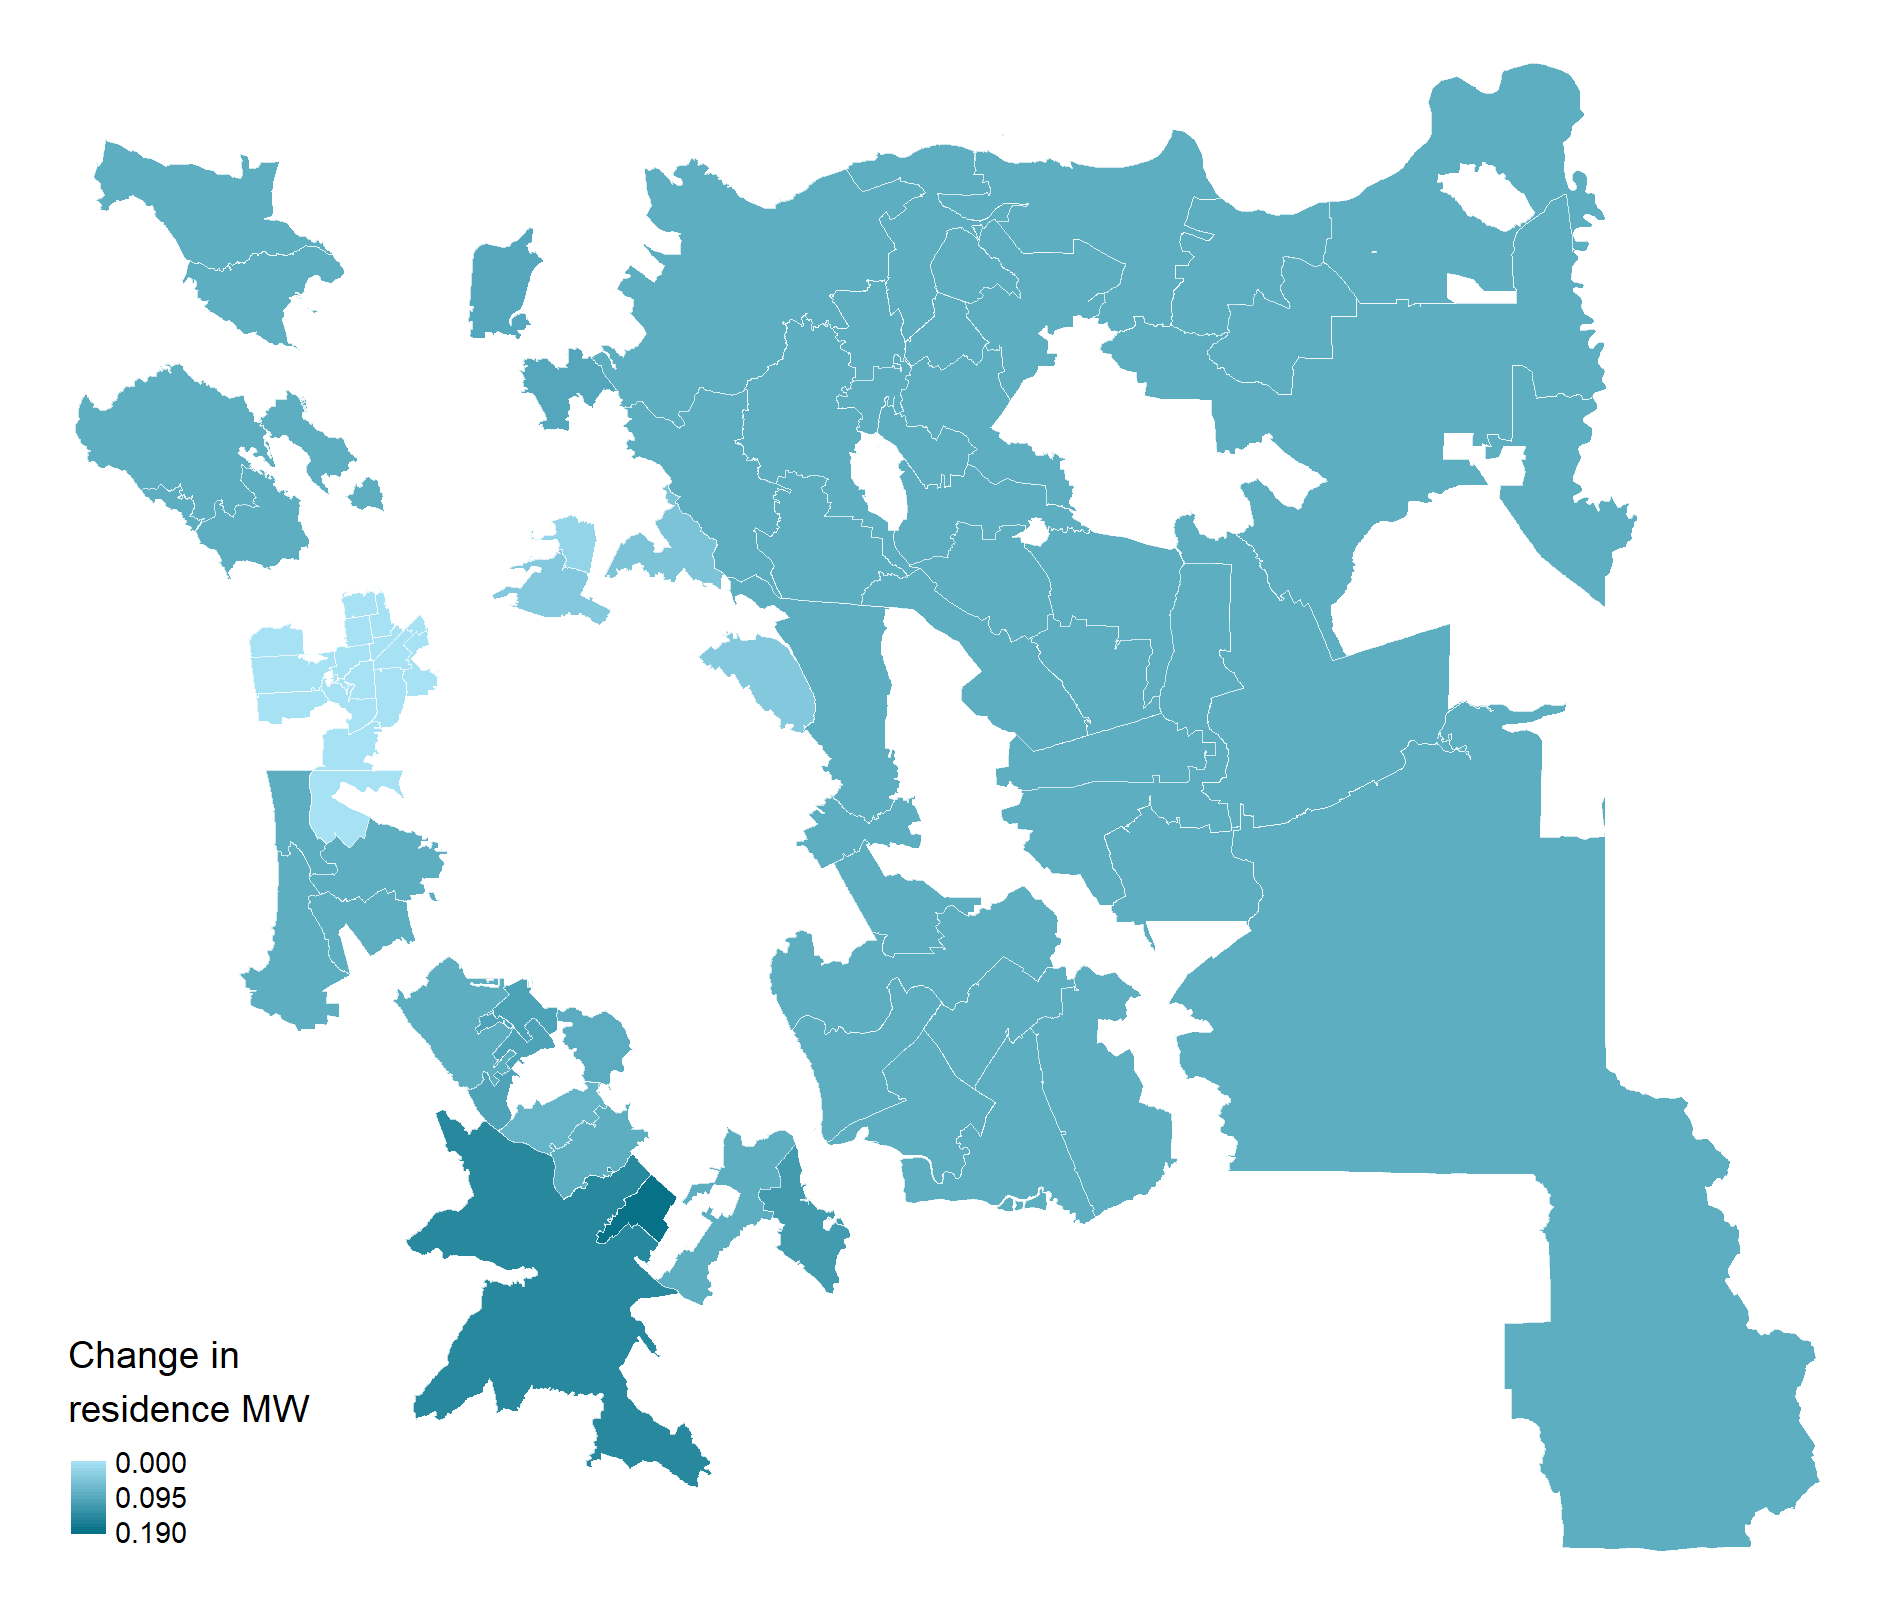
\includegraphics[scale = 0.36]{maps_events/output/bay_area_2018-12_statutory_mw.png}
            \end{figure}   
        \end{column}
        \begin{column}{0.50\textwidth}
            \vspace{-4mm}
            \begin{figure}
                \centering
                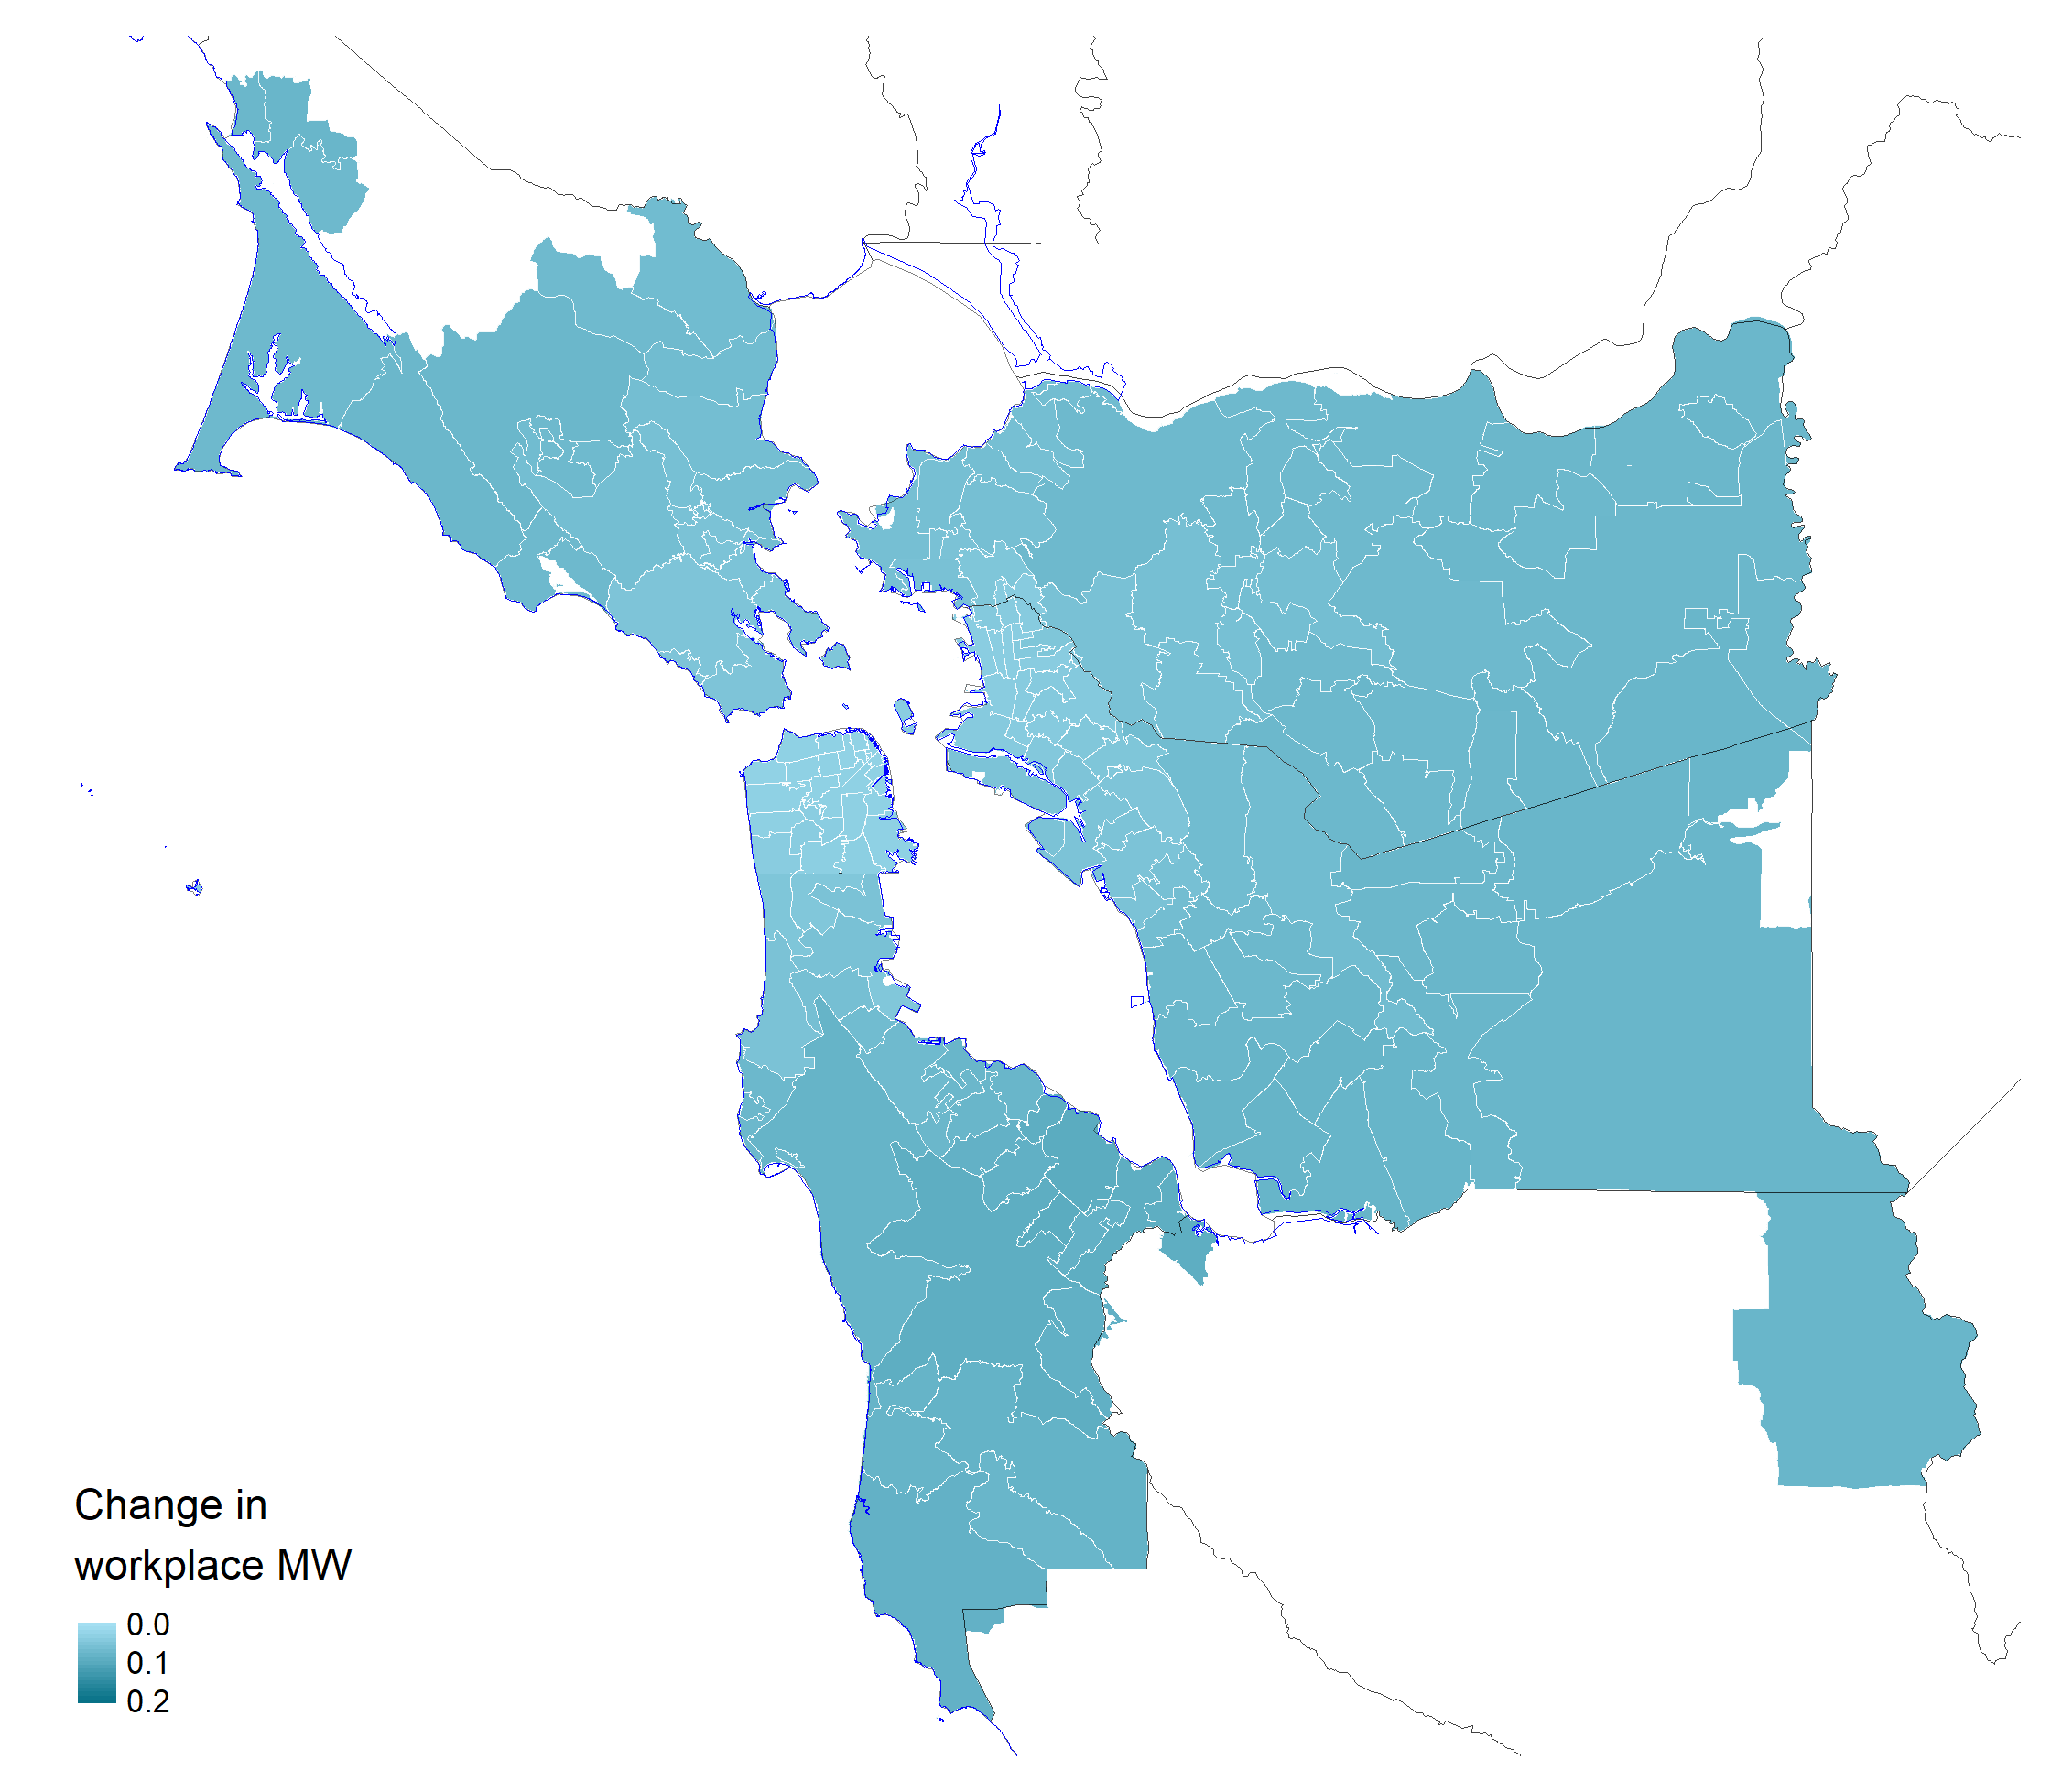
\includegraphics[scale = 0.36]{maps_events/output/bay_area2018-12_wkp_mw.png}
            \end{figure}   
        \end{column}
    \end{columns}
    \hyperlink{chi_example}{\beamerbutton{Go back}}
\end{frame}


\begin{frame}[label = san_diego_example]
\frametitle{San Diego (MW changes in January 2019)}
    \begin{columns}
        \begin{column}{0.50\textwidth}
            \vspace{-4mm}
            \begin{figure}
                \centering
                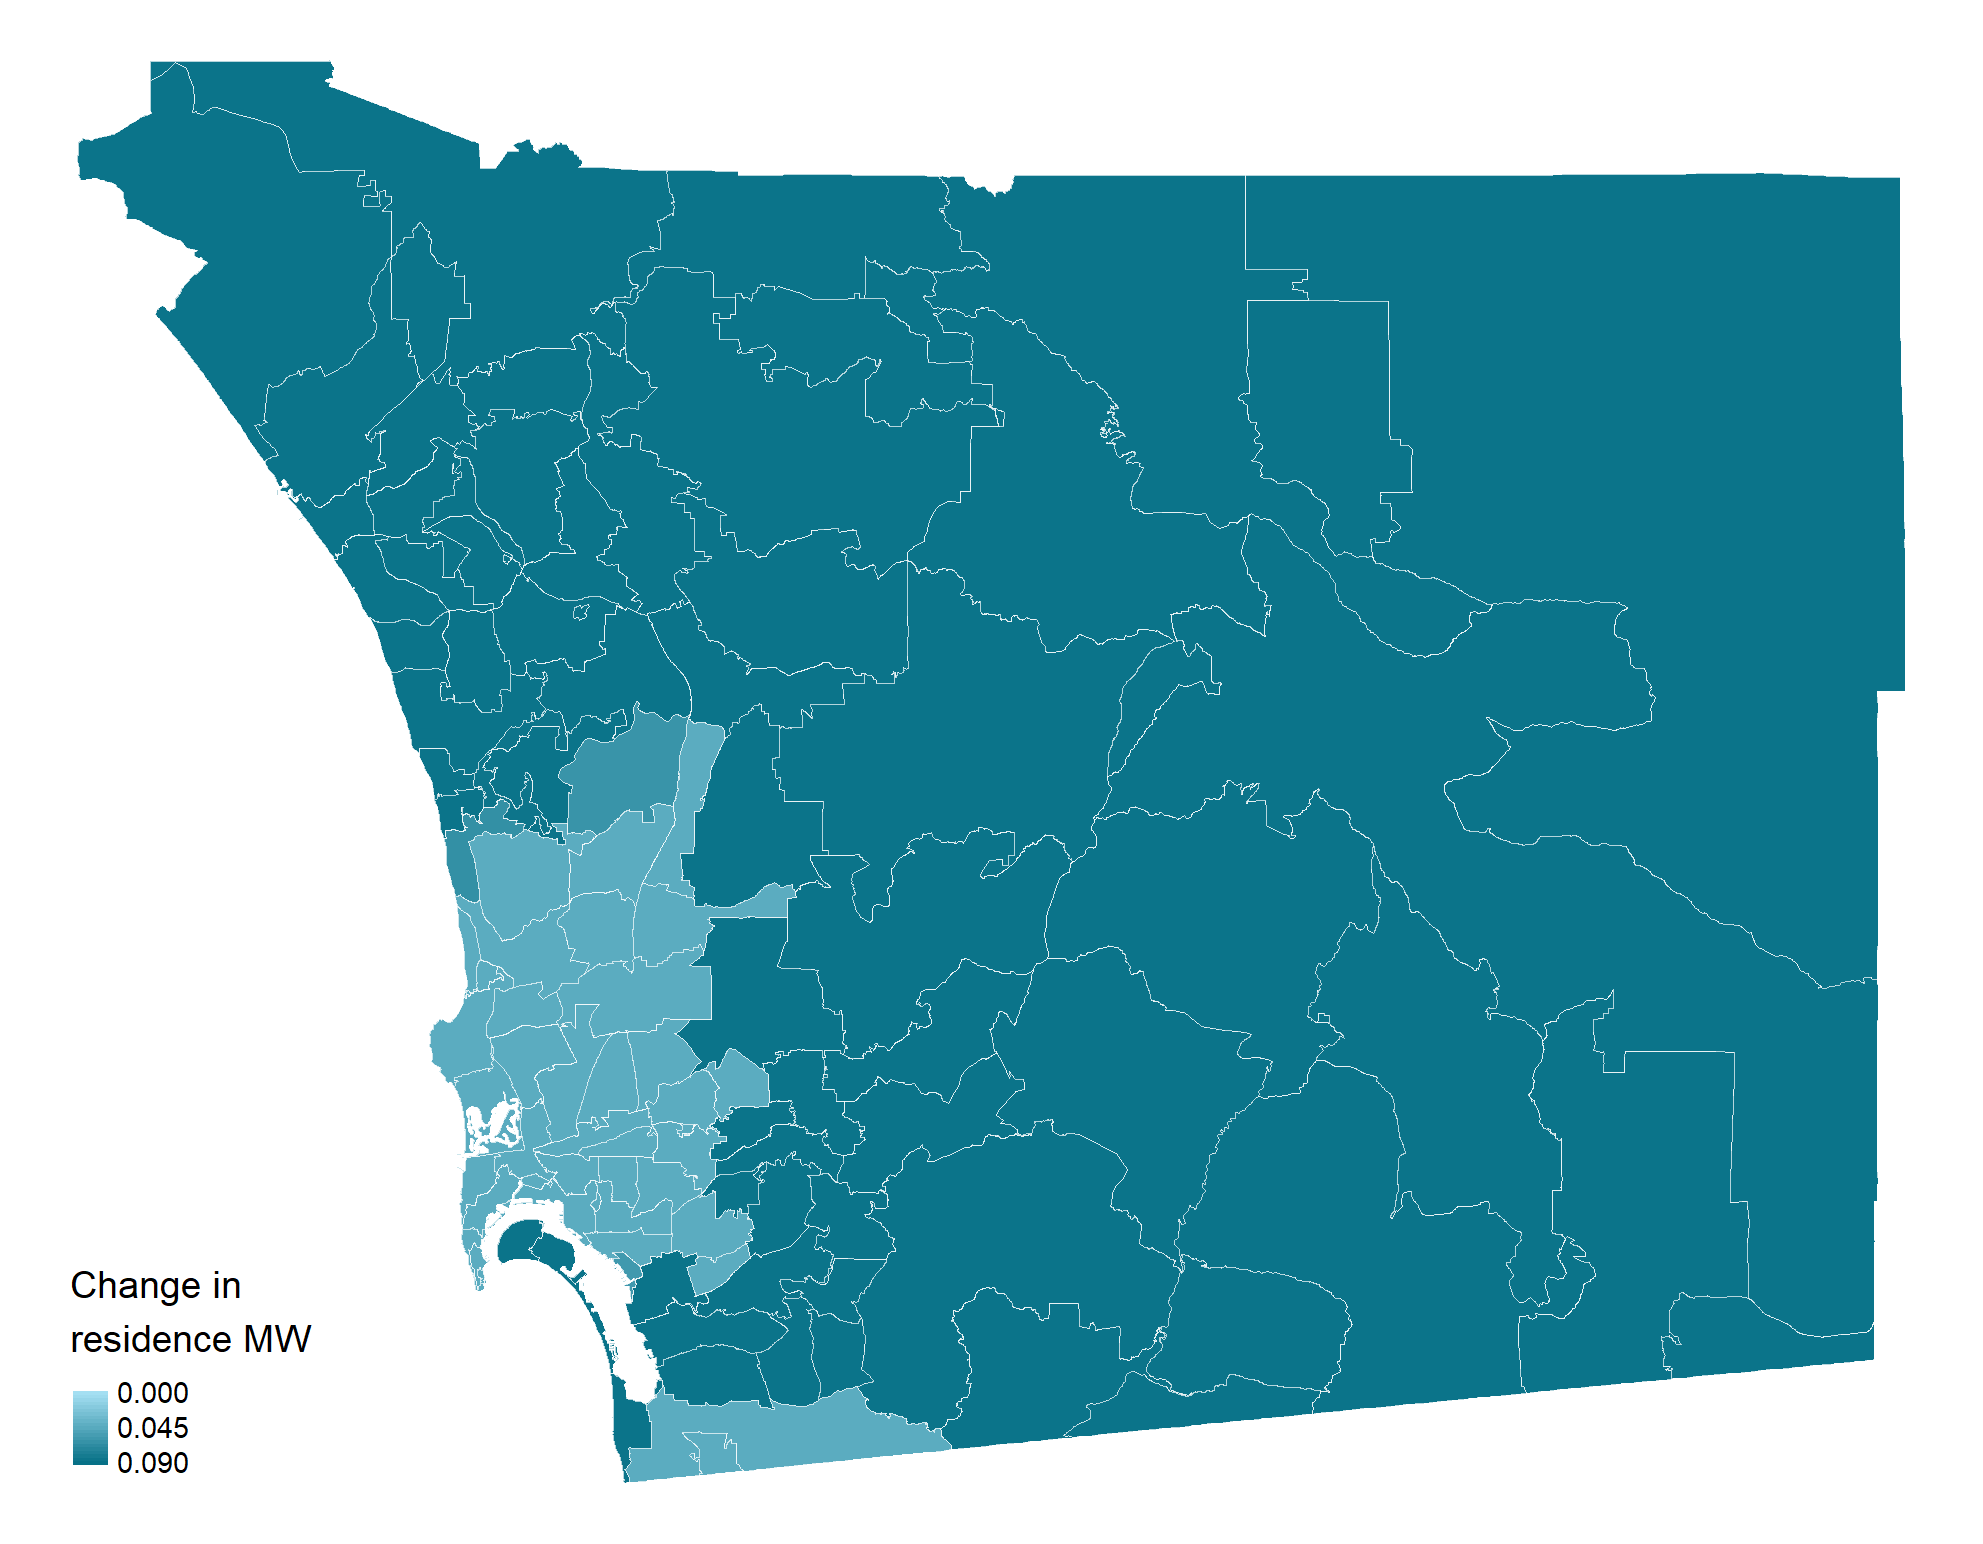
\includegraphics[scale = 0.3]{maps_events/output/san_diego_2018-12_statutory_mw.png}
            \end{figure}   
        \end{column}
        \begin{column}{0.50\textwidth}
            \vspace{-4mm}
            \begin{figure}
                \centering
                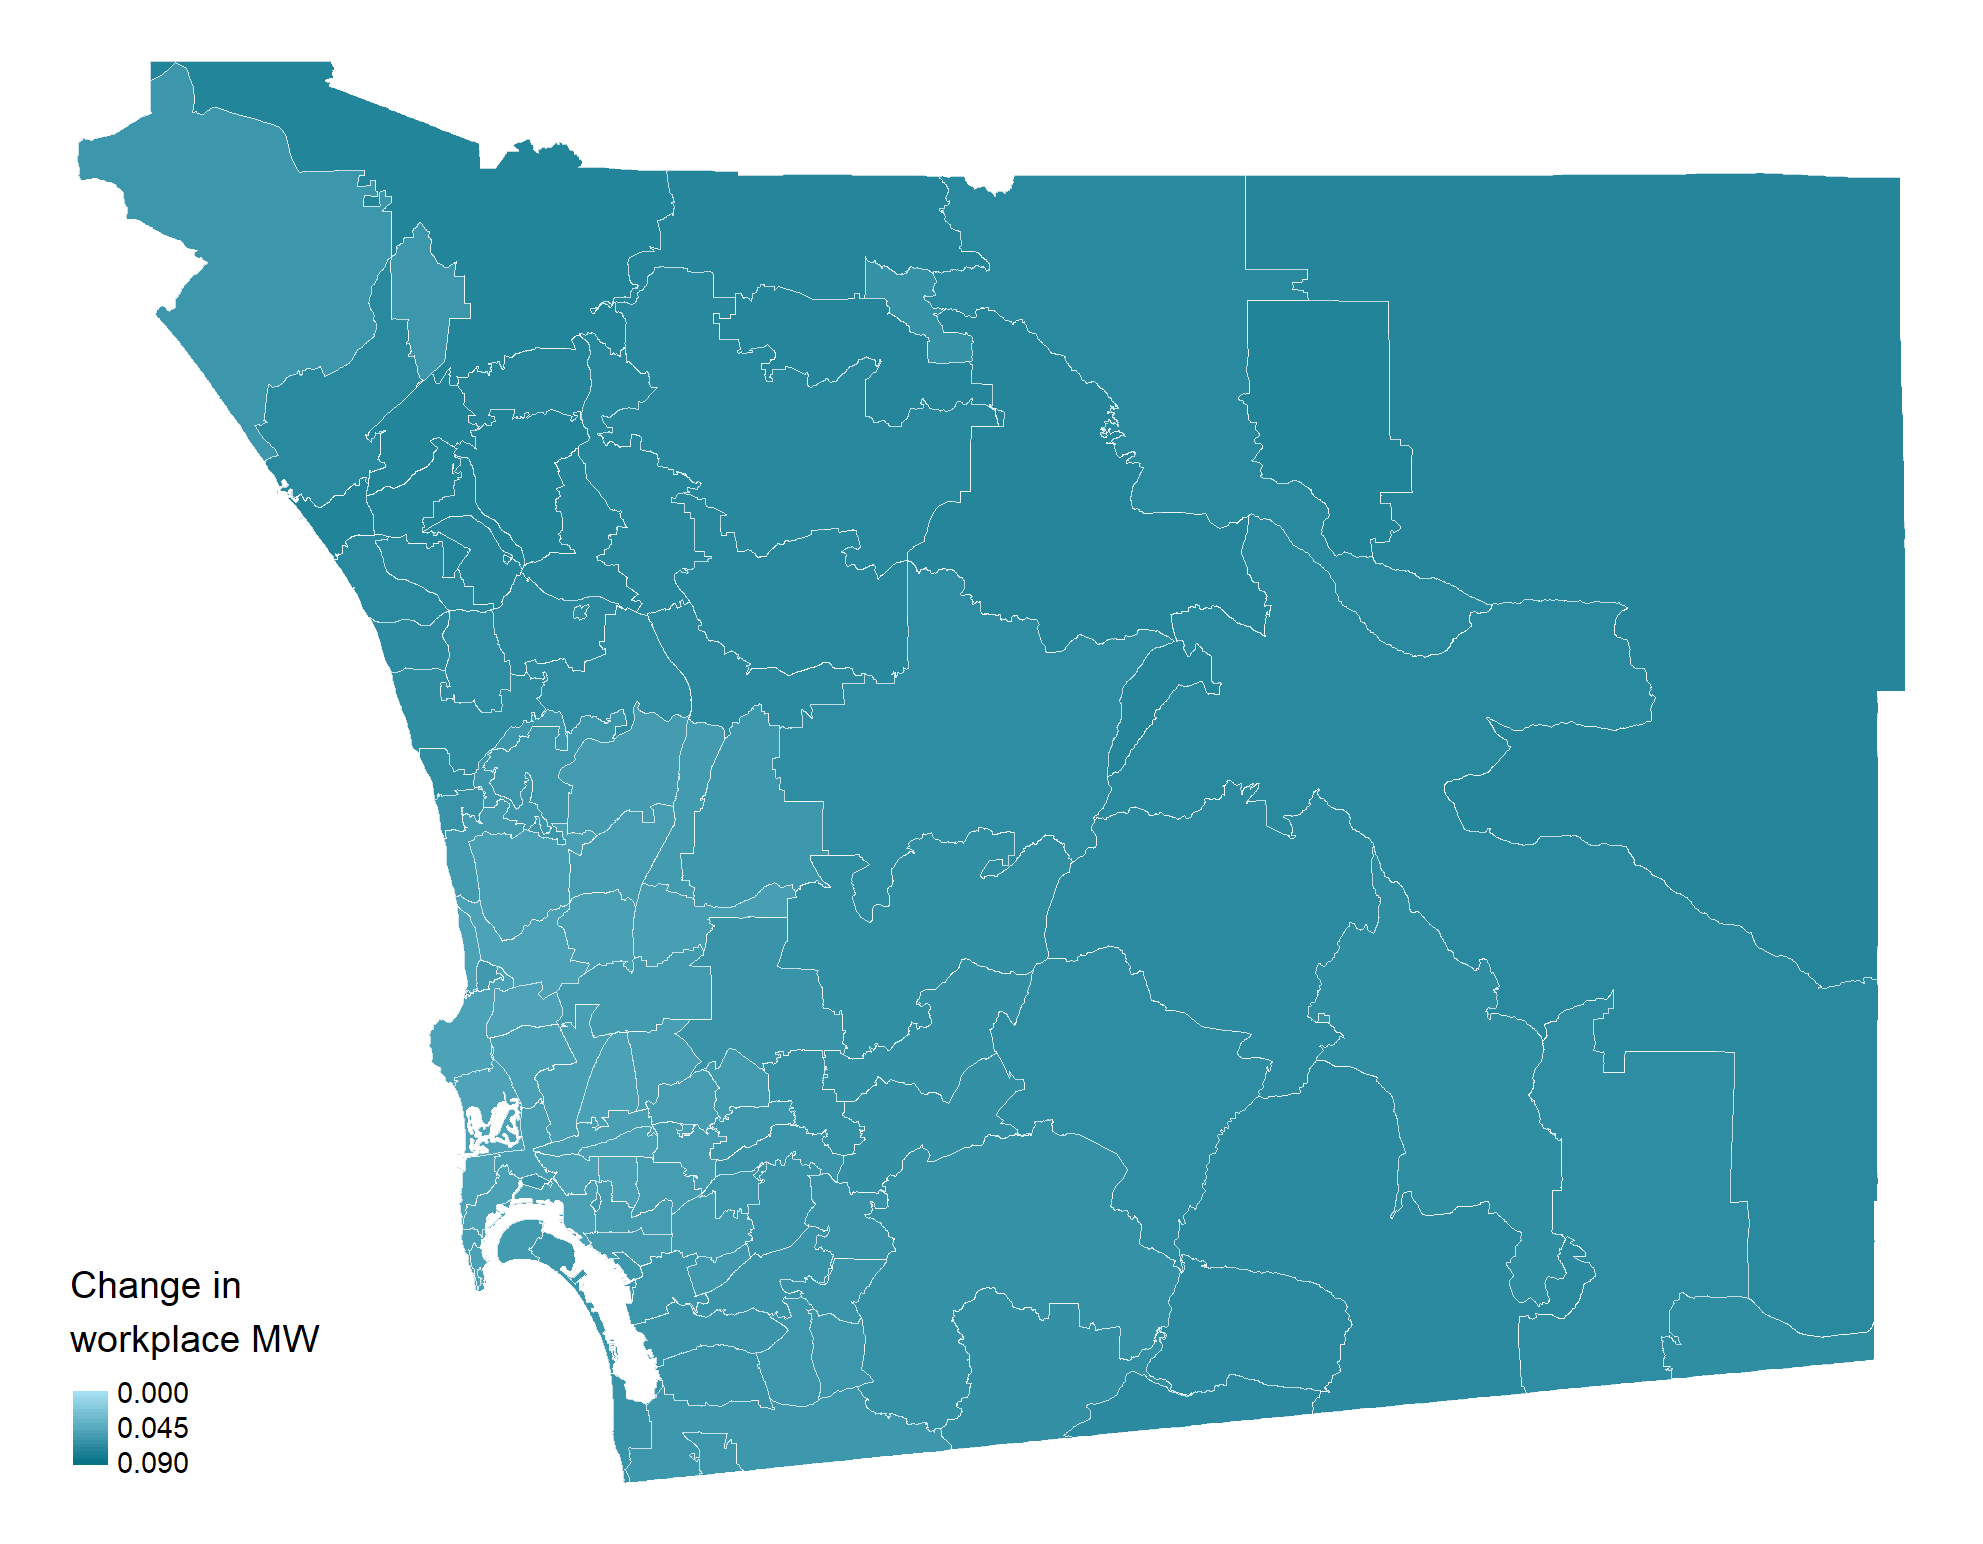
\includegraphics[scale = 0.3]{maps_events/output/san_diego2018-12_wkp_mw.png}
            \end{figure}   
        \end{column}
    \end{columns}
     \hyperlink{chi_example}{\beamerbutton{Go back}}
\end{frame}

\begin{frame}[label = kc_example]
\frametitle{Kansas City (MW changes in January 2019)}
    \begin{columns}
        \begin{column}{0.50\textwidth}
            \vspace{-4mm}
            \begin{figure}
                \centering
                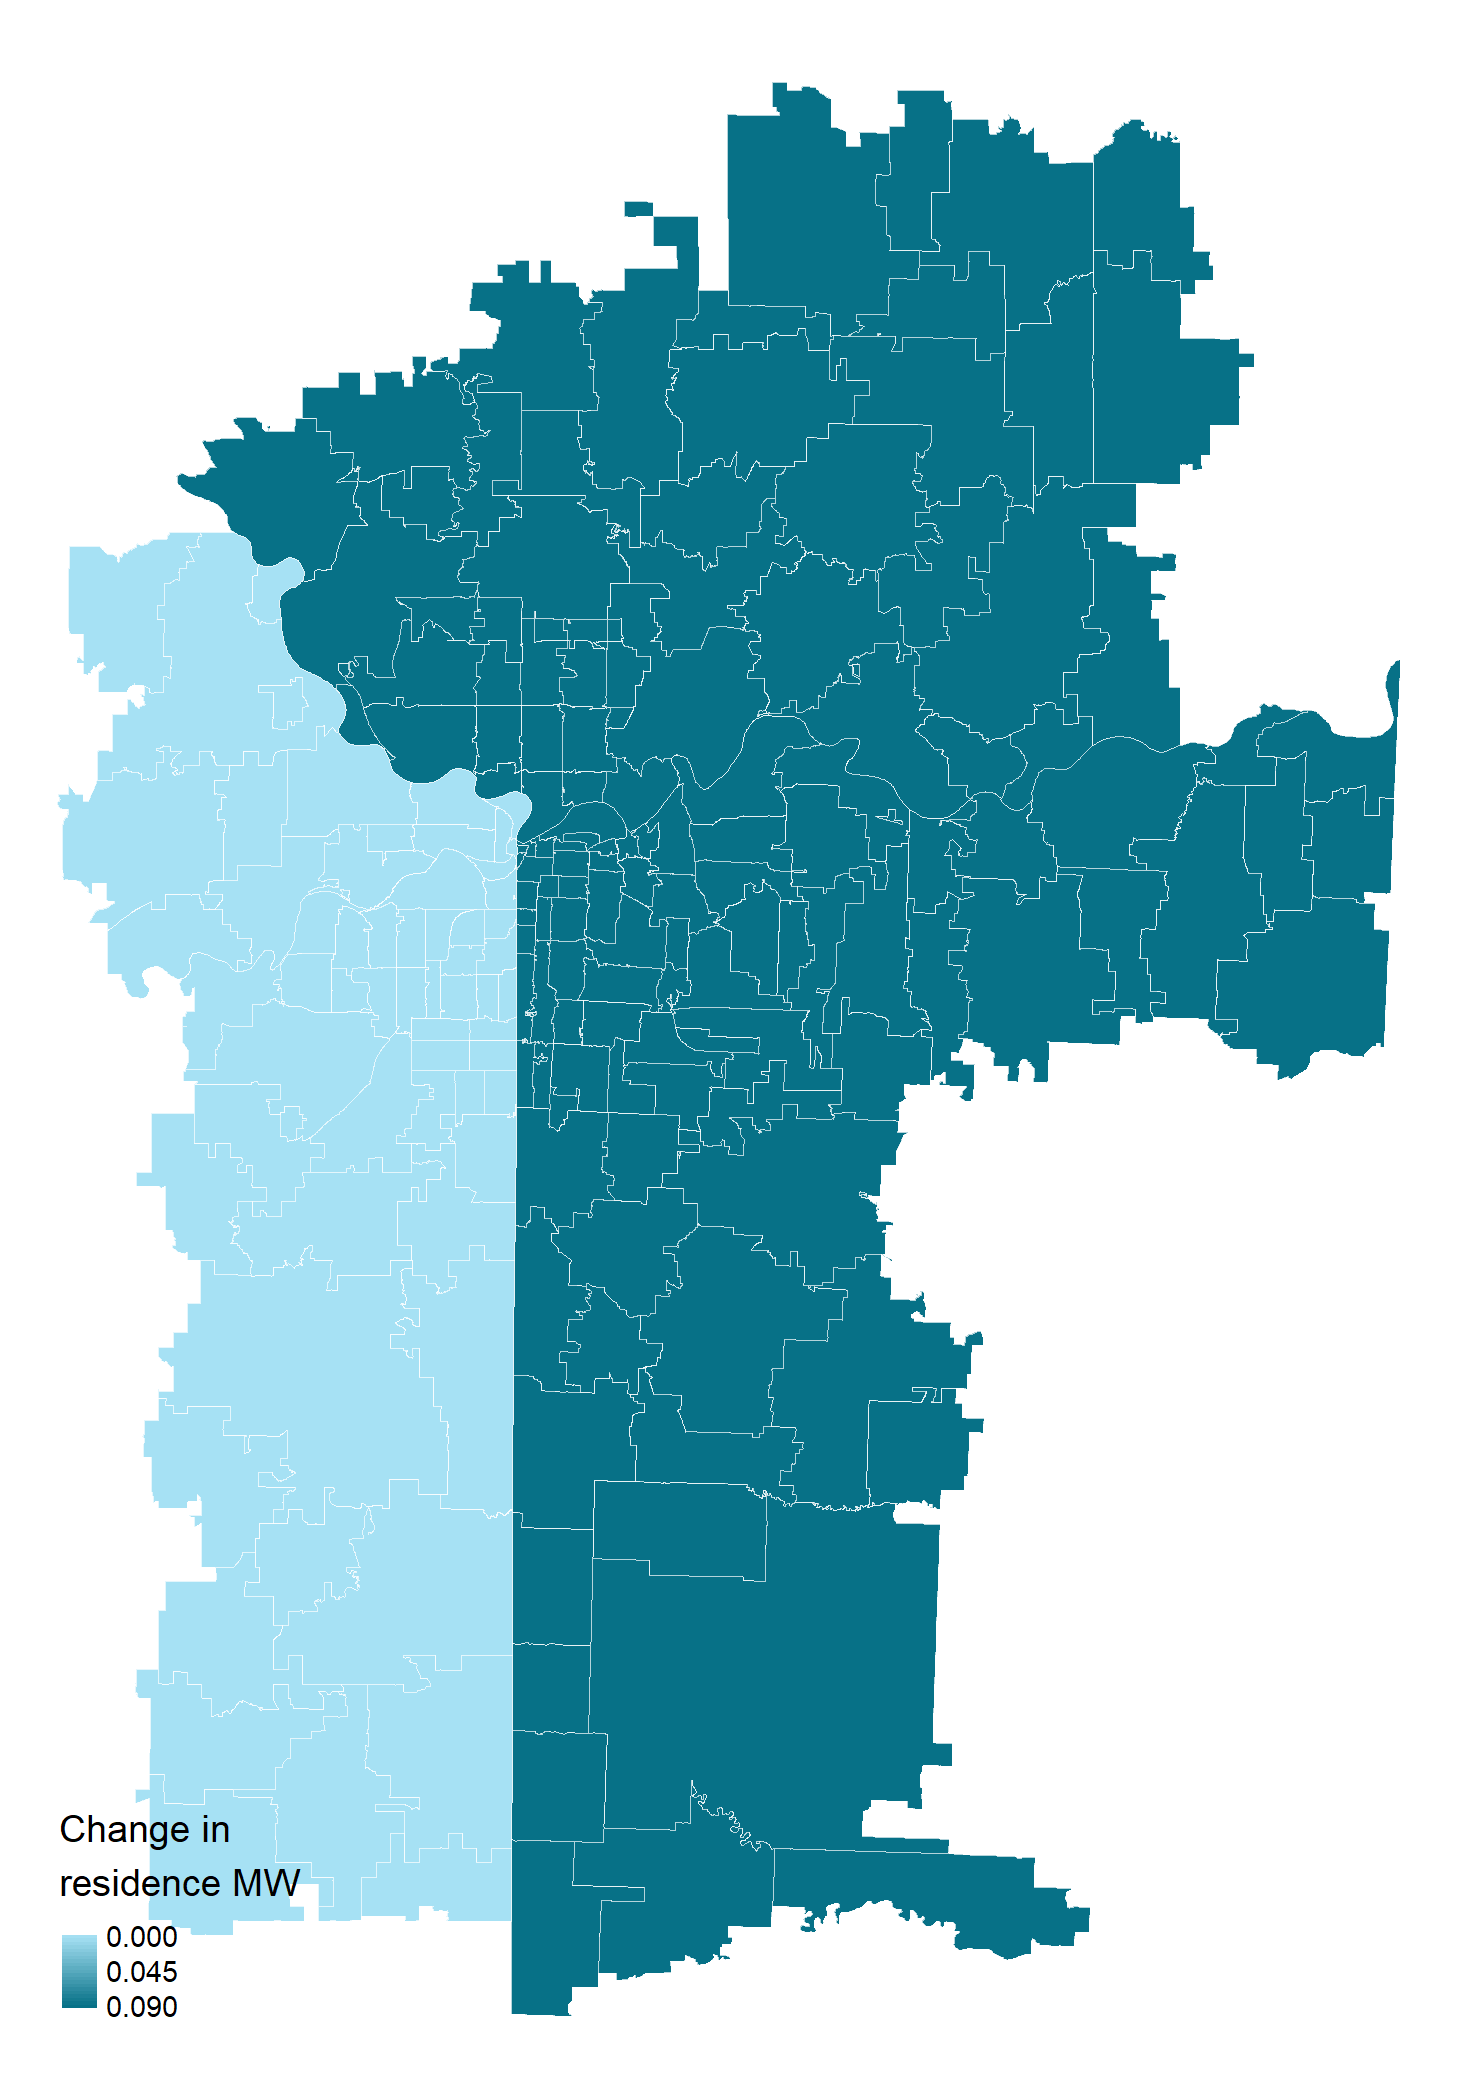
\includegraphics[scale = 0.3]{maps_events/output/kc_2018-12_statutory_mw.png}
            \end{figure}   
        \end{column}
        \begin{column}{0.50\textwidth}
            \vspace{-4mm}
            \begin{figure}
                \centering
                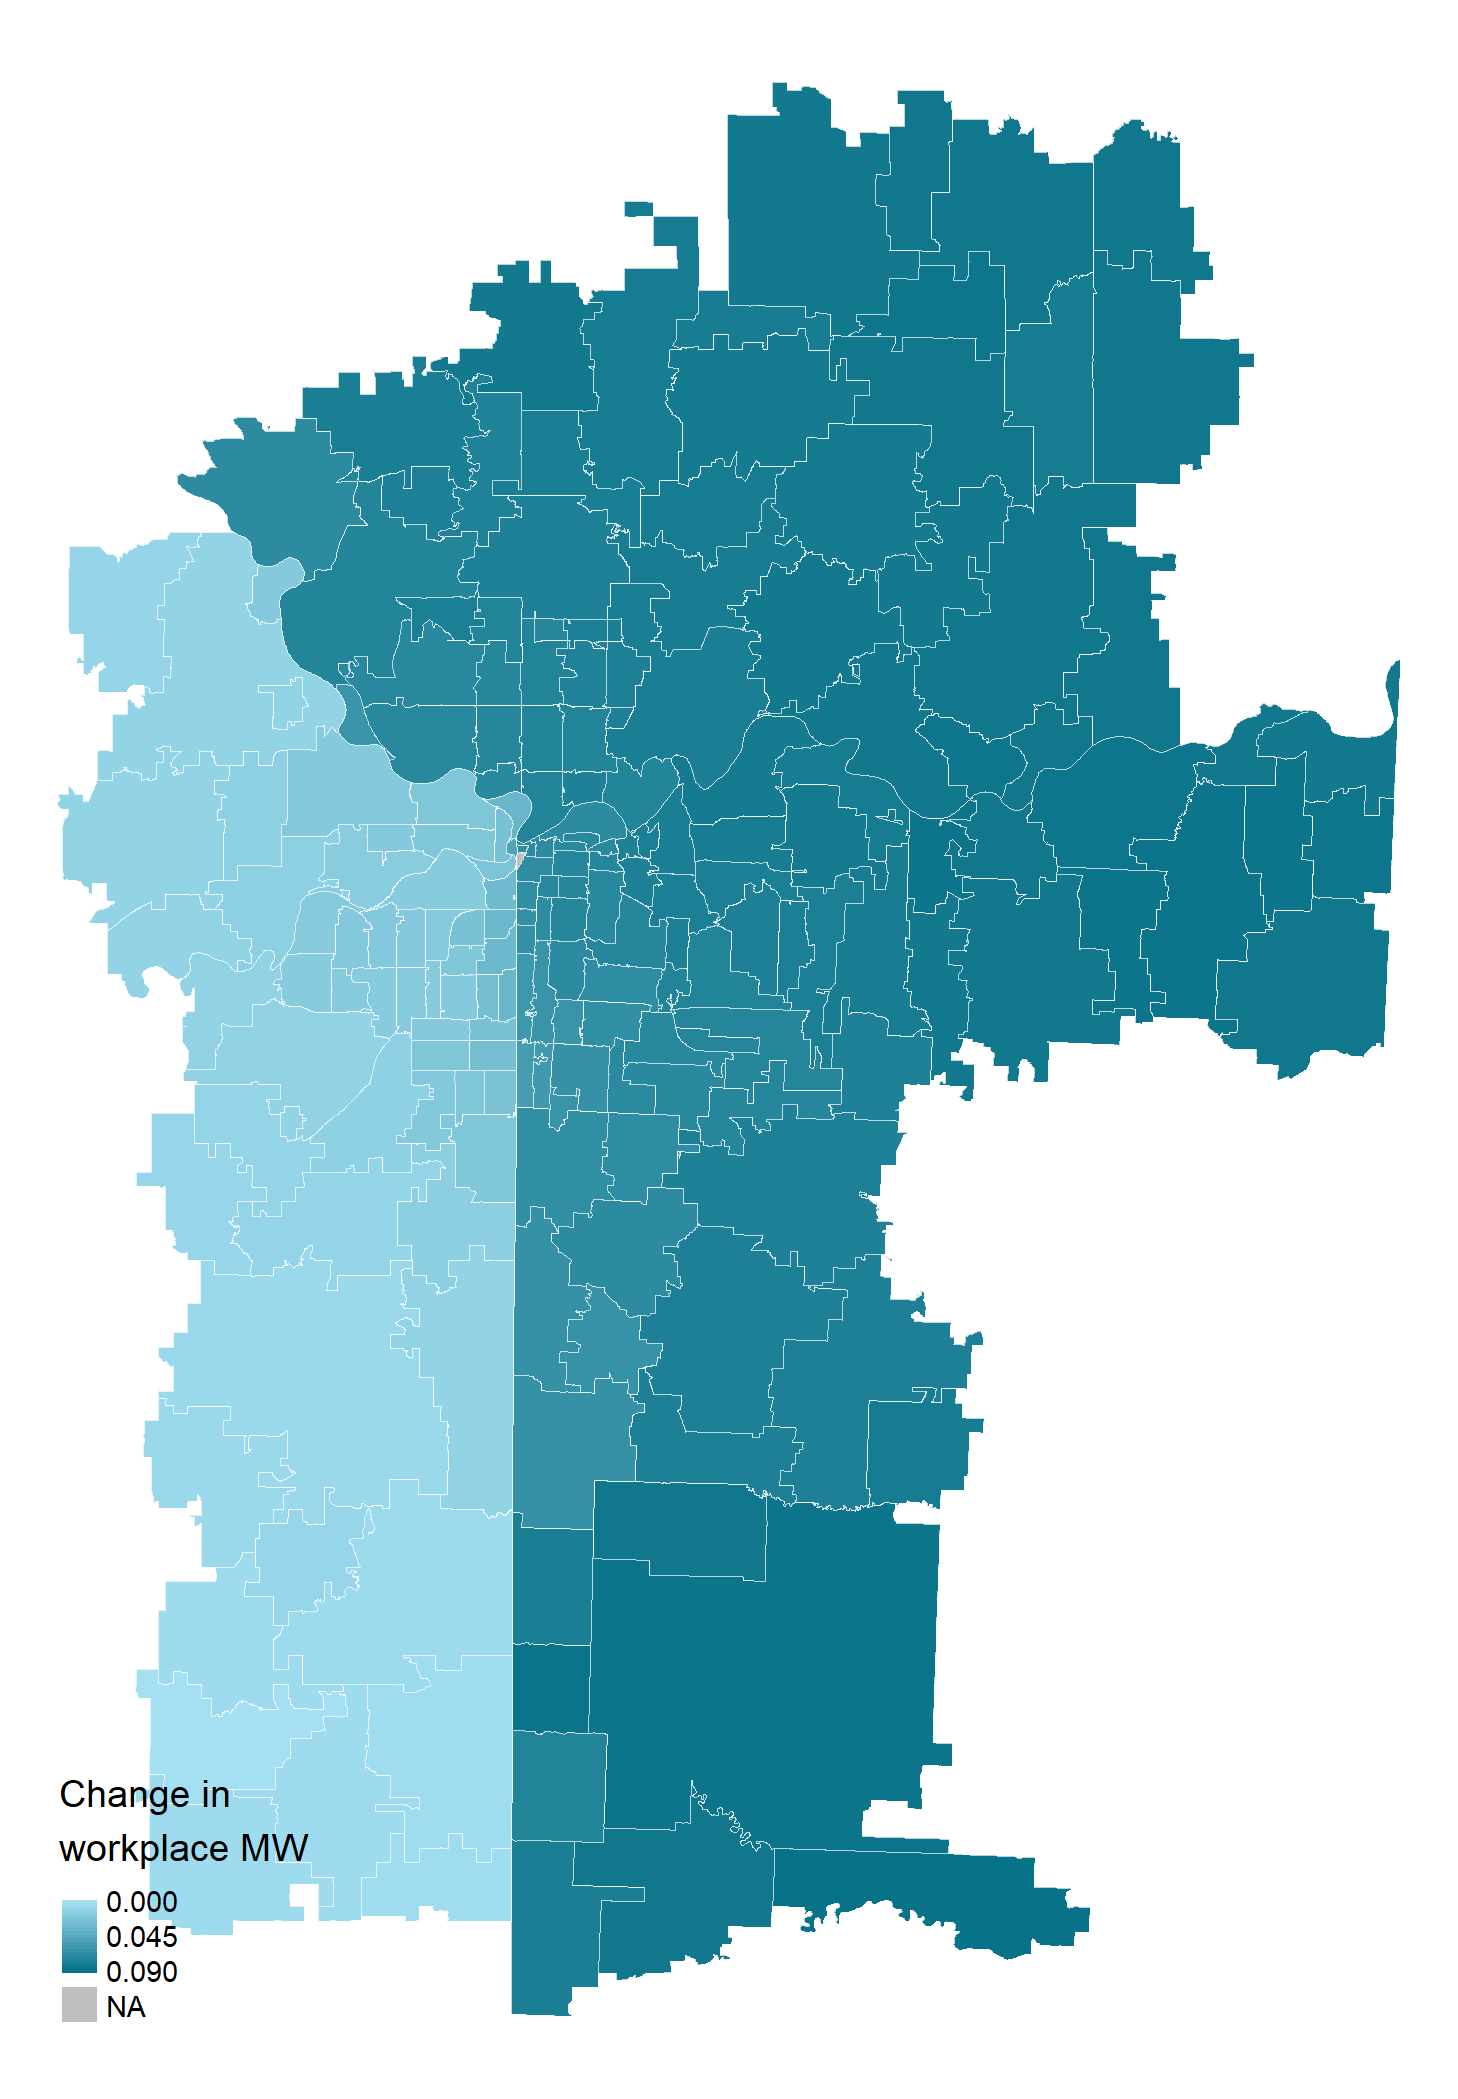
\includegraphics[scale = 0.3]{maps_events/output/kc2018-12_wkp_mw.png}
            \end{figure}   
        \end{column}
    \end{columns}
     \hyperlink{chi_example}{\beamerbutton{Go back}}
\end{frame}

\begin{frame}[label = zillow_pop_density]
    \frametitle{Comparison between Zillow Sample and Population Density}
    \begin{figure}
        \centering
    \vspace{10mm}
    \hspace{-23mm}
        \begin{subfigure}{0.41\textwidth}
            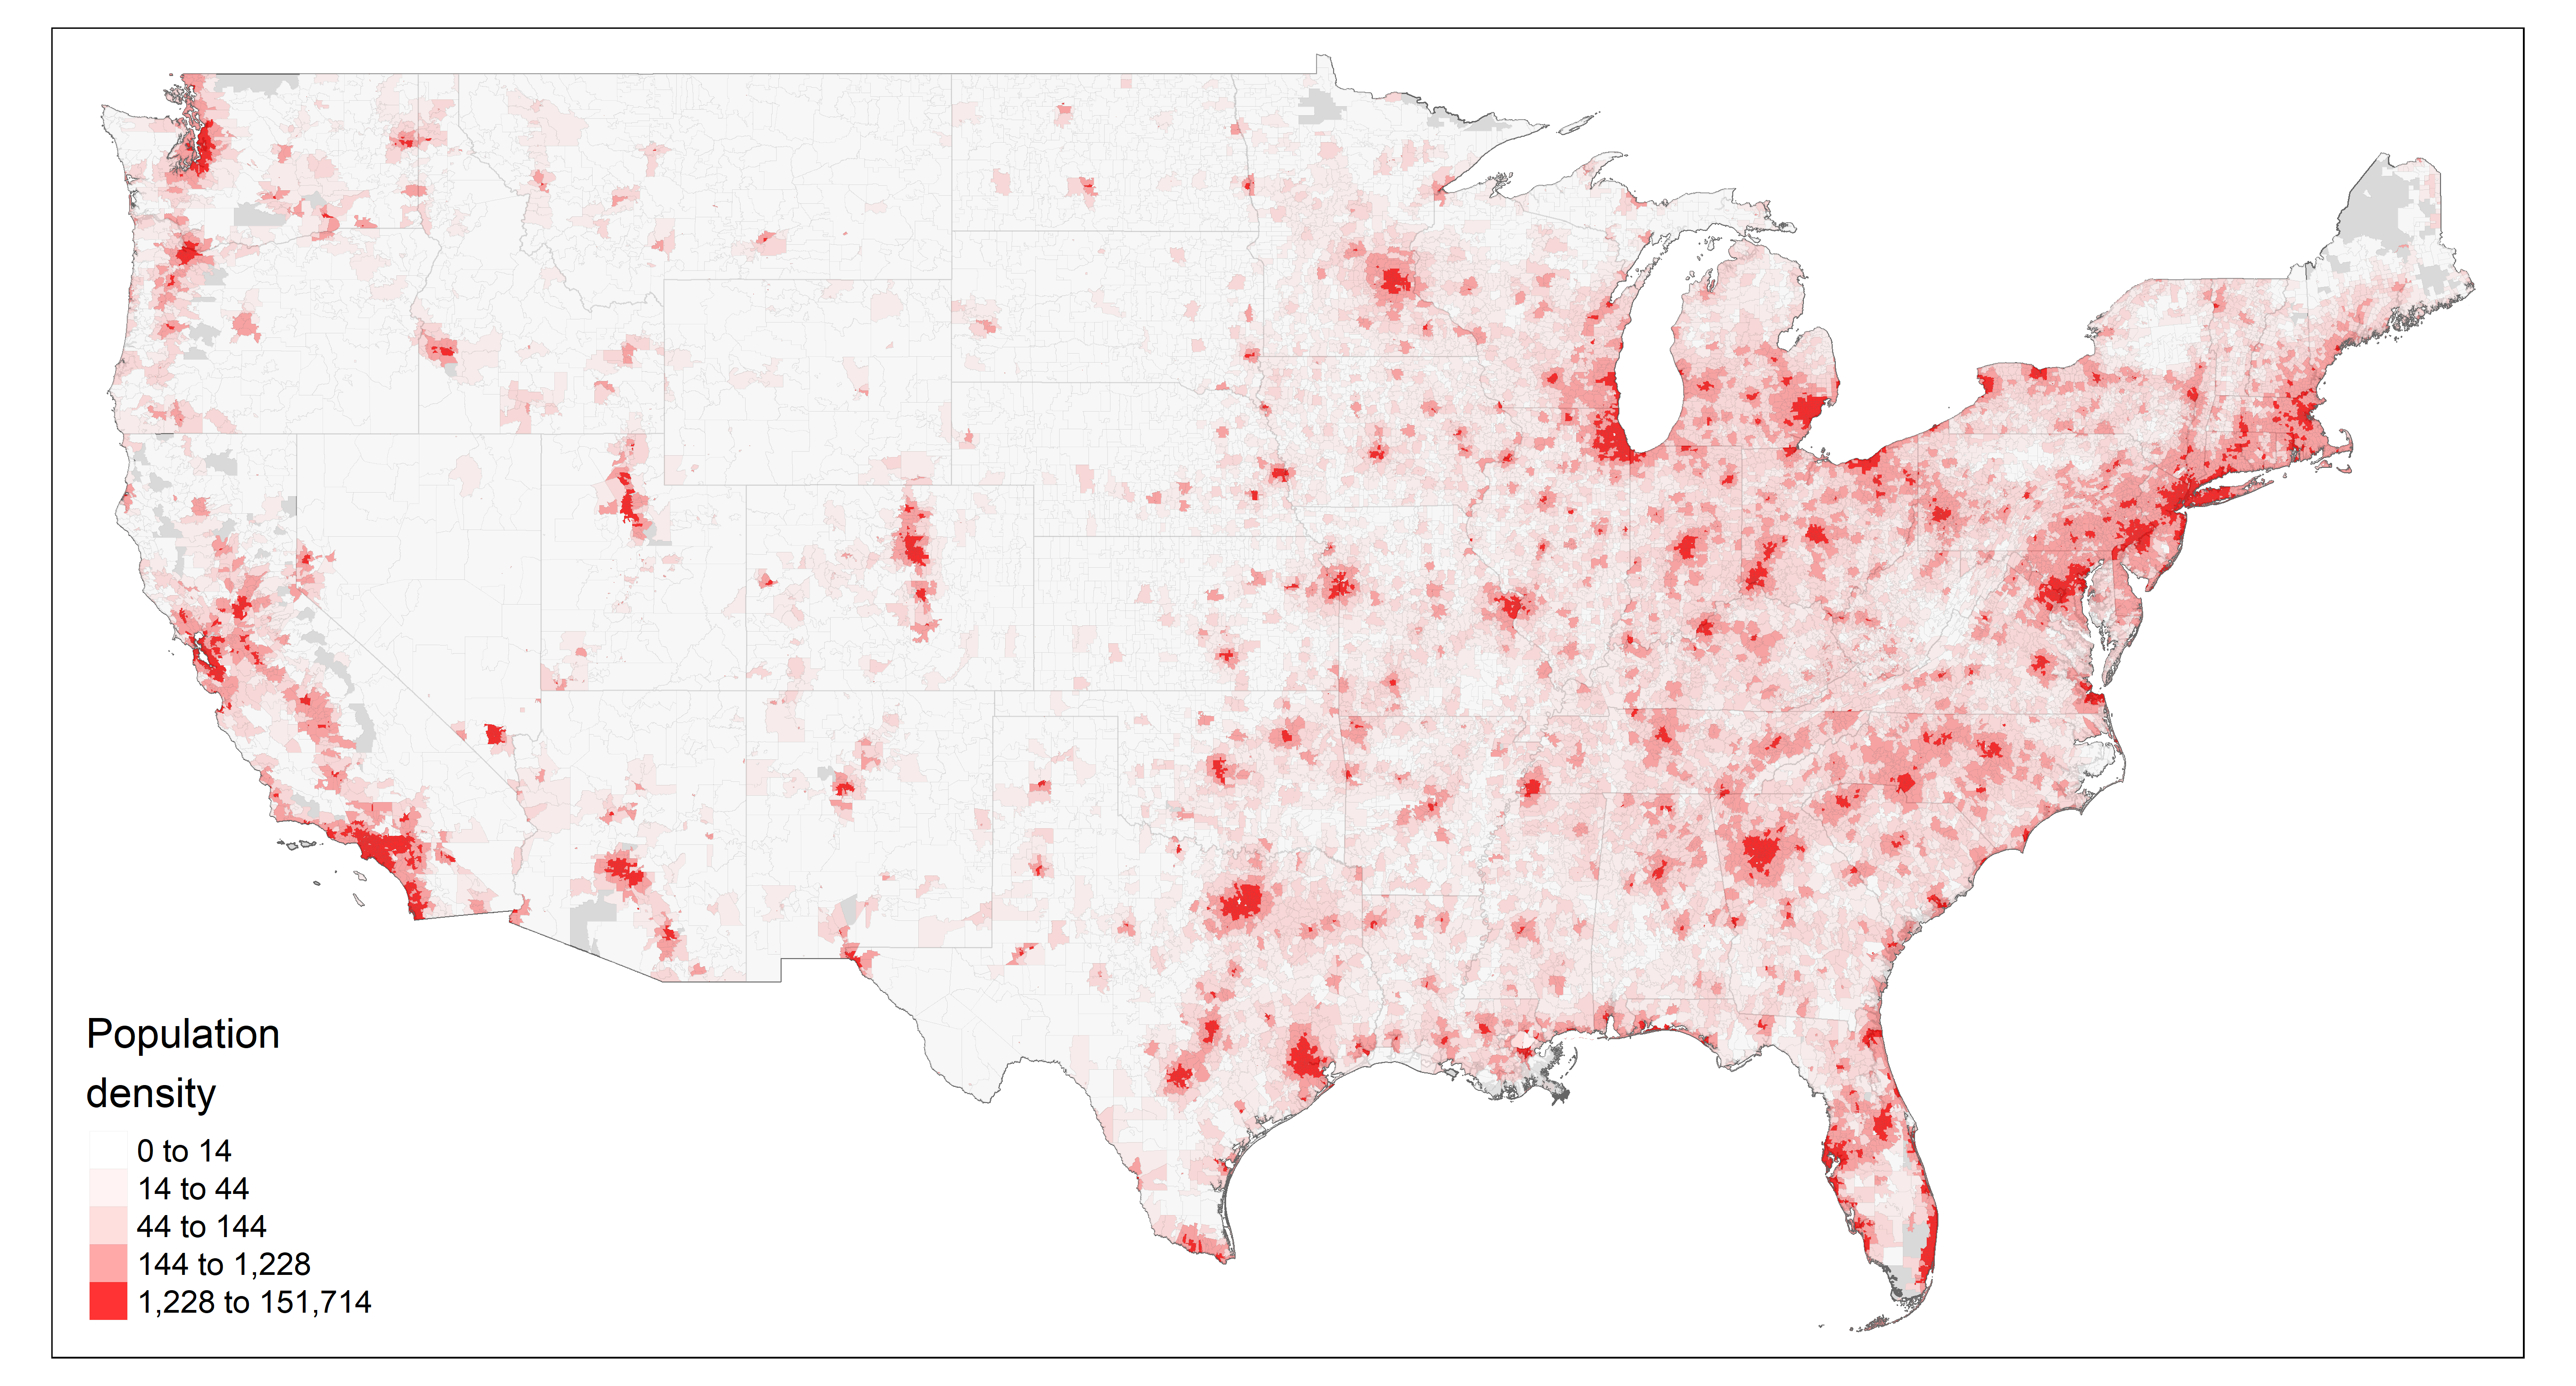
\includegraphics[scale = 0.33]{maps_US/output/USPS_zipcodes_pop_density.png}
        \end{subfigure}%
    \quad\quad\quad\quad\quad\quad
        \begin{subfigure}{0.41\textwidth}
            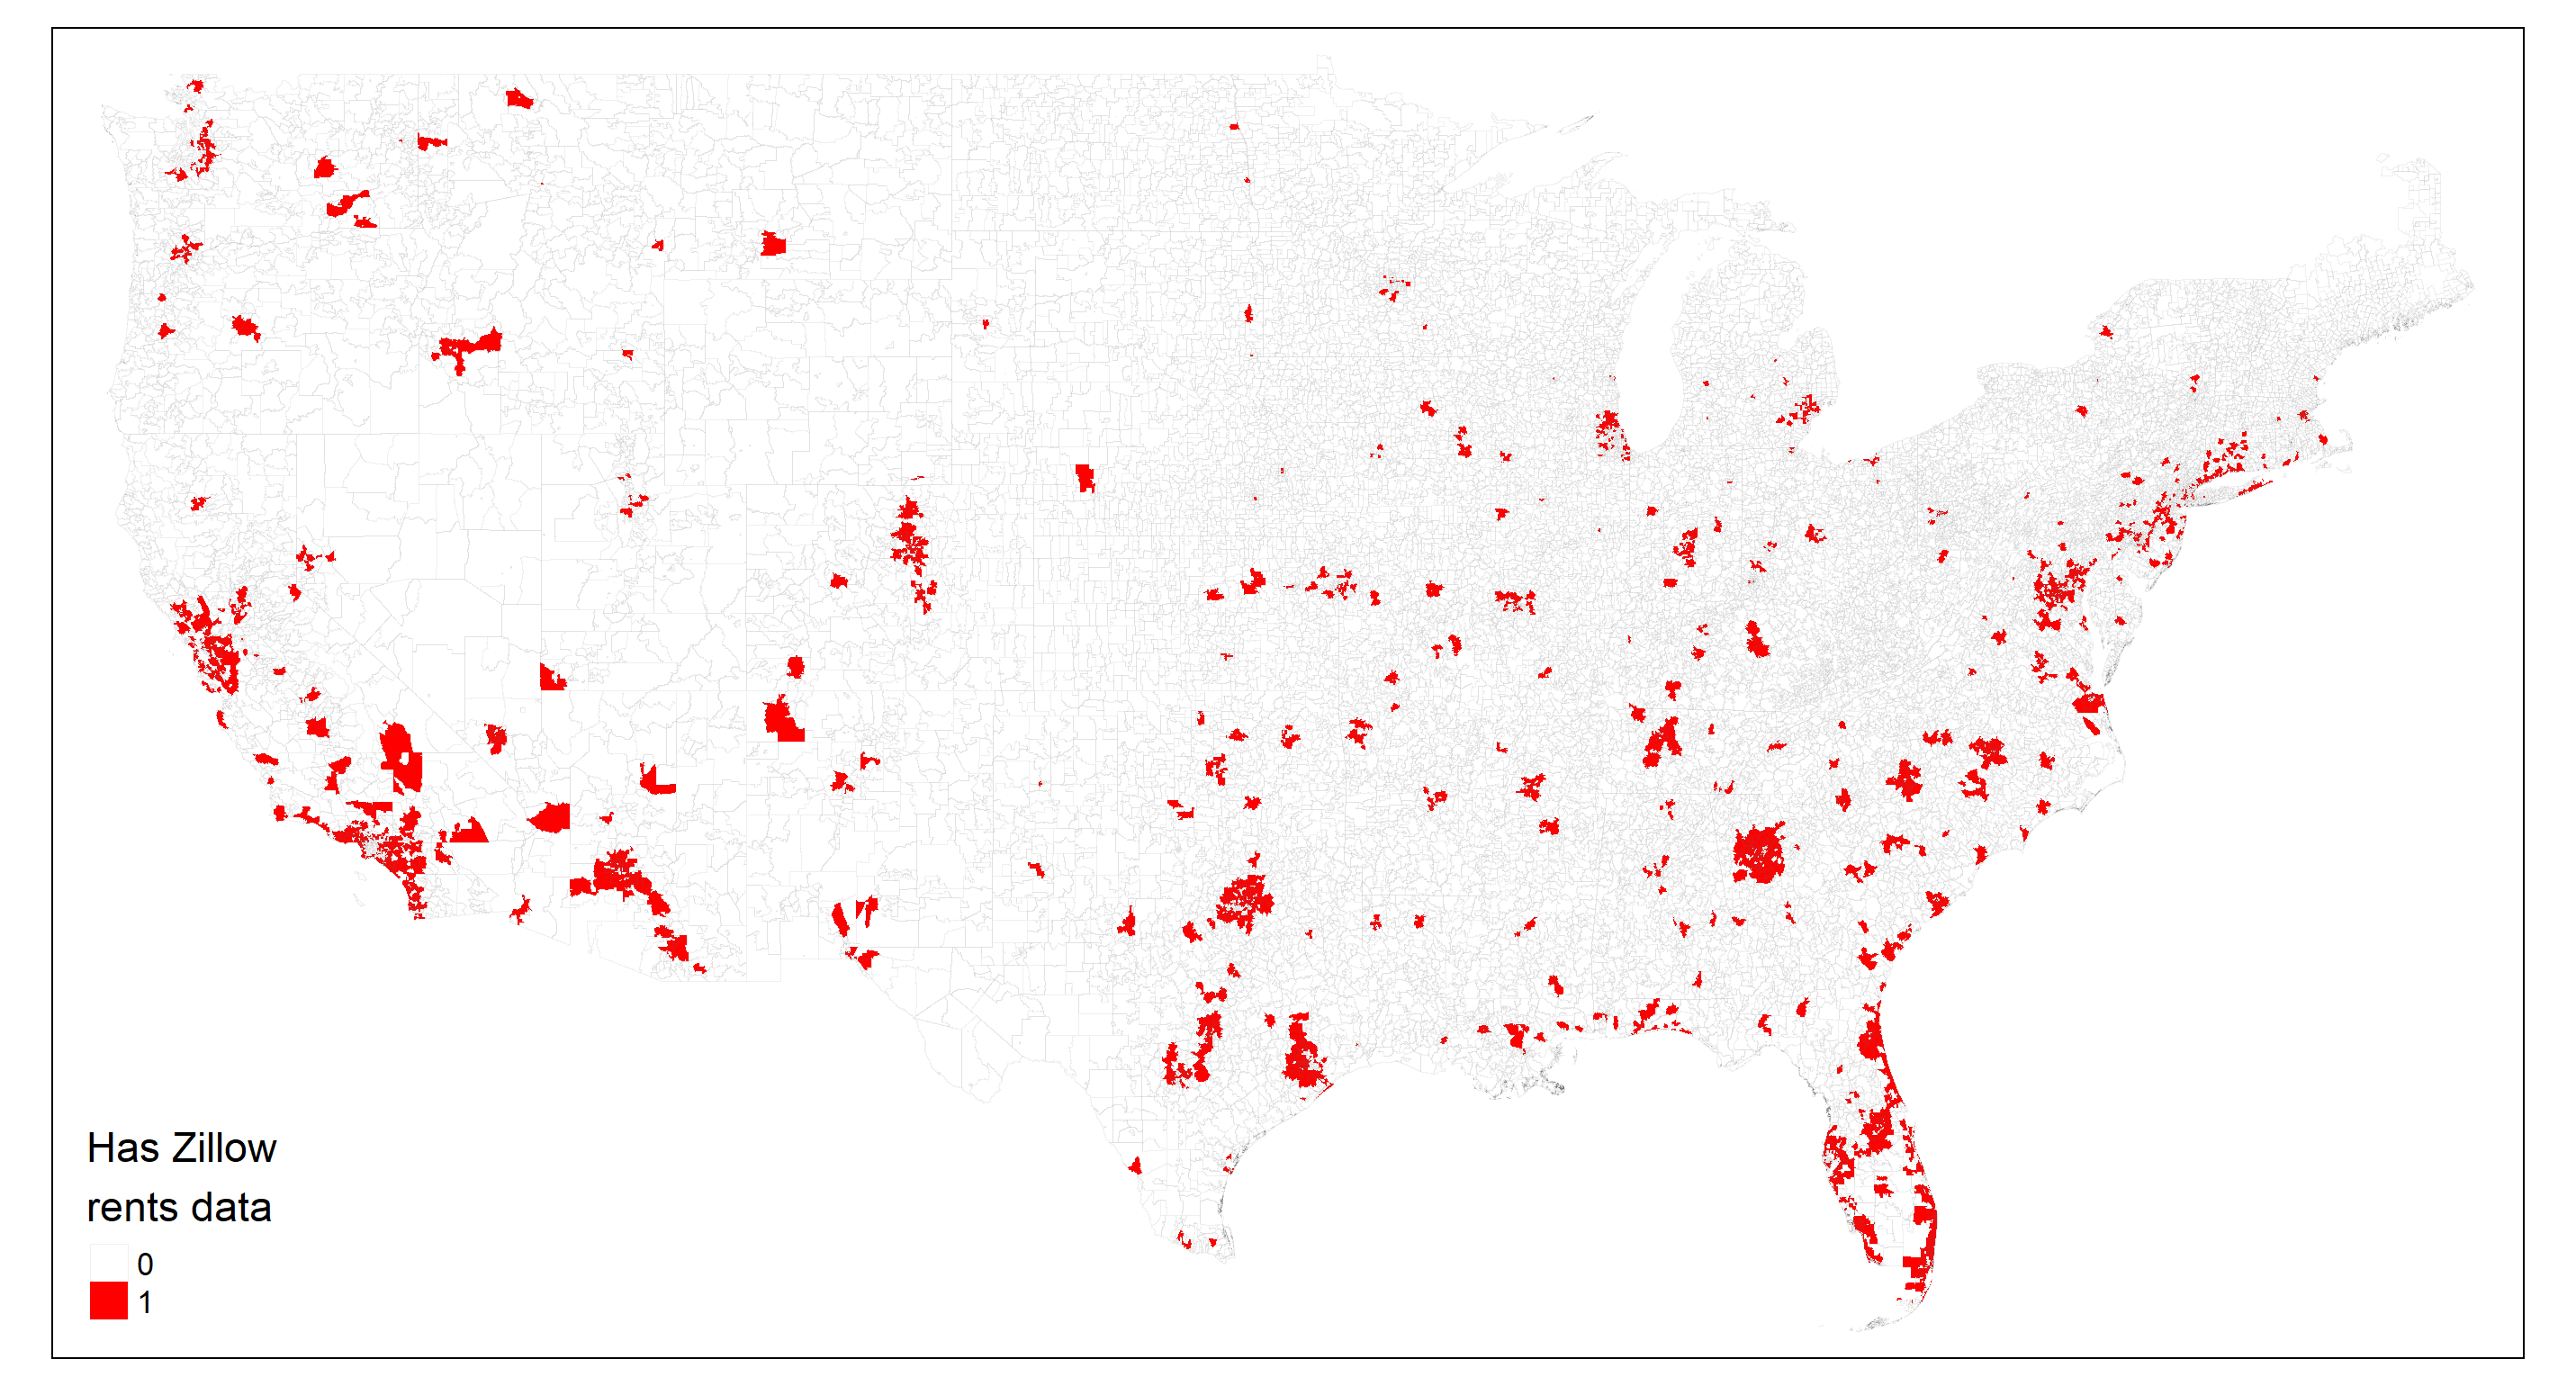
\includegraphics[scale = 0.33]{maps_US/output/USPS_zipcodes_zillow_data.png}
        \end{subfigure}
    \end{figure}
    \hyperlink{zillow_data}{\beamerbutton{Go Back}}
\end{frame}

\begin{frame}[label=mw_changes_map]
    \frametitle{MW changes between Jan 2010 and Dec 2019, mainland US}

    \vspace{2mm}
    \begin{figure}        
        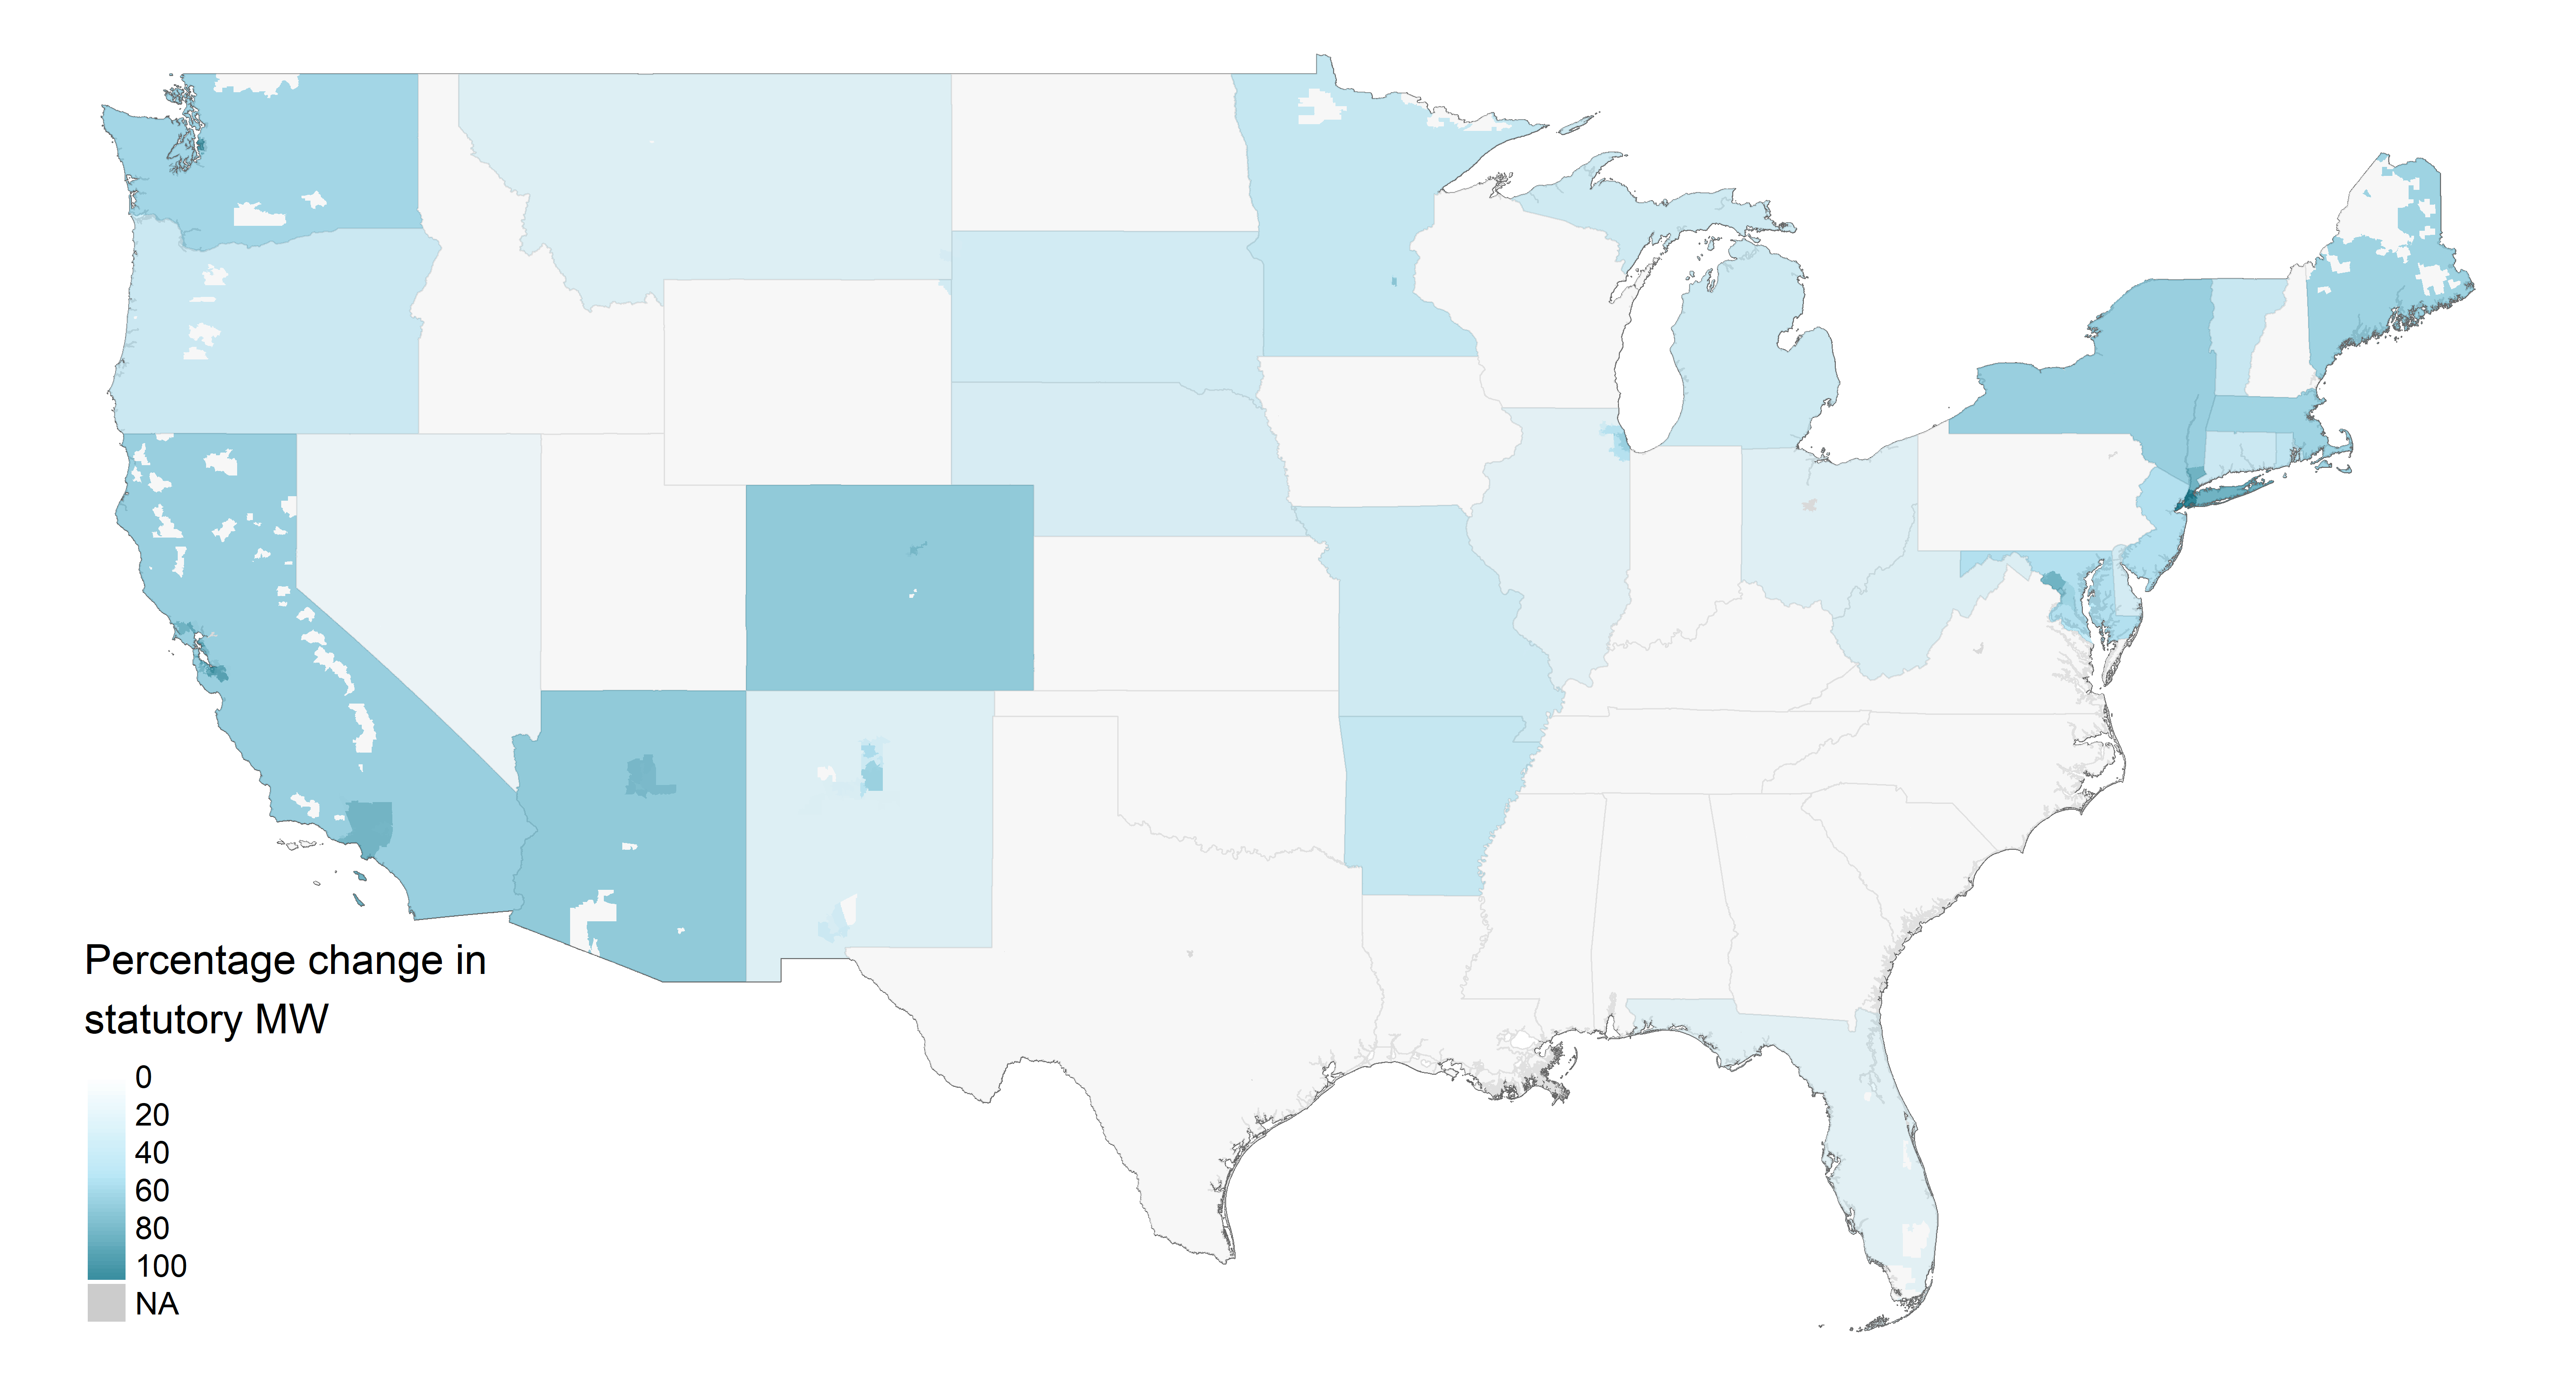
\includegraphics[width = 0.84\textwidth]{maps_mw_long_run/output/USchange_perc_statutory_mw.png}
    \end{figure}
    
    \hyperlink{dist_mw_changes}{\beamerbutton{Go Back}}
\end{frame}

\begin{frame}[label = exclude_res]
    \frametitle{Excluding residence MW}

    \begin{figure}
        \centering
        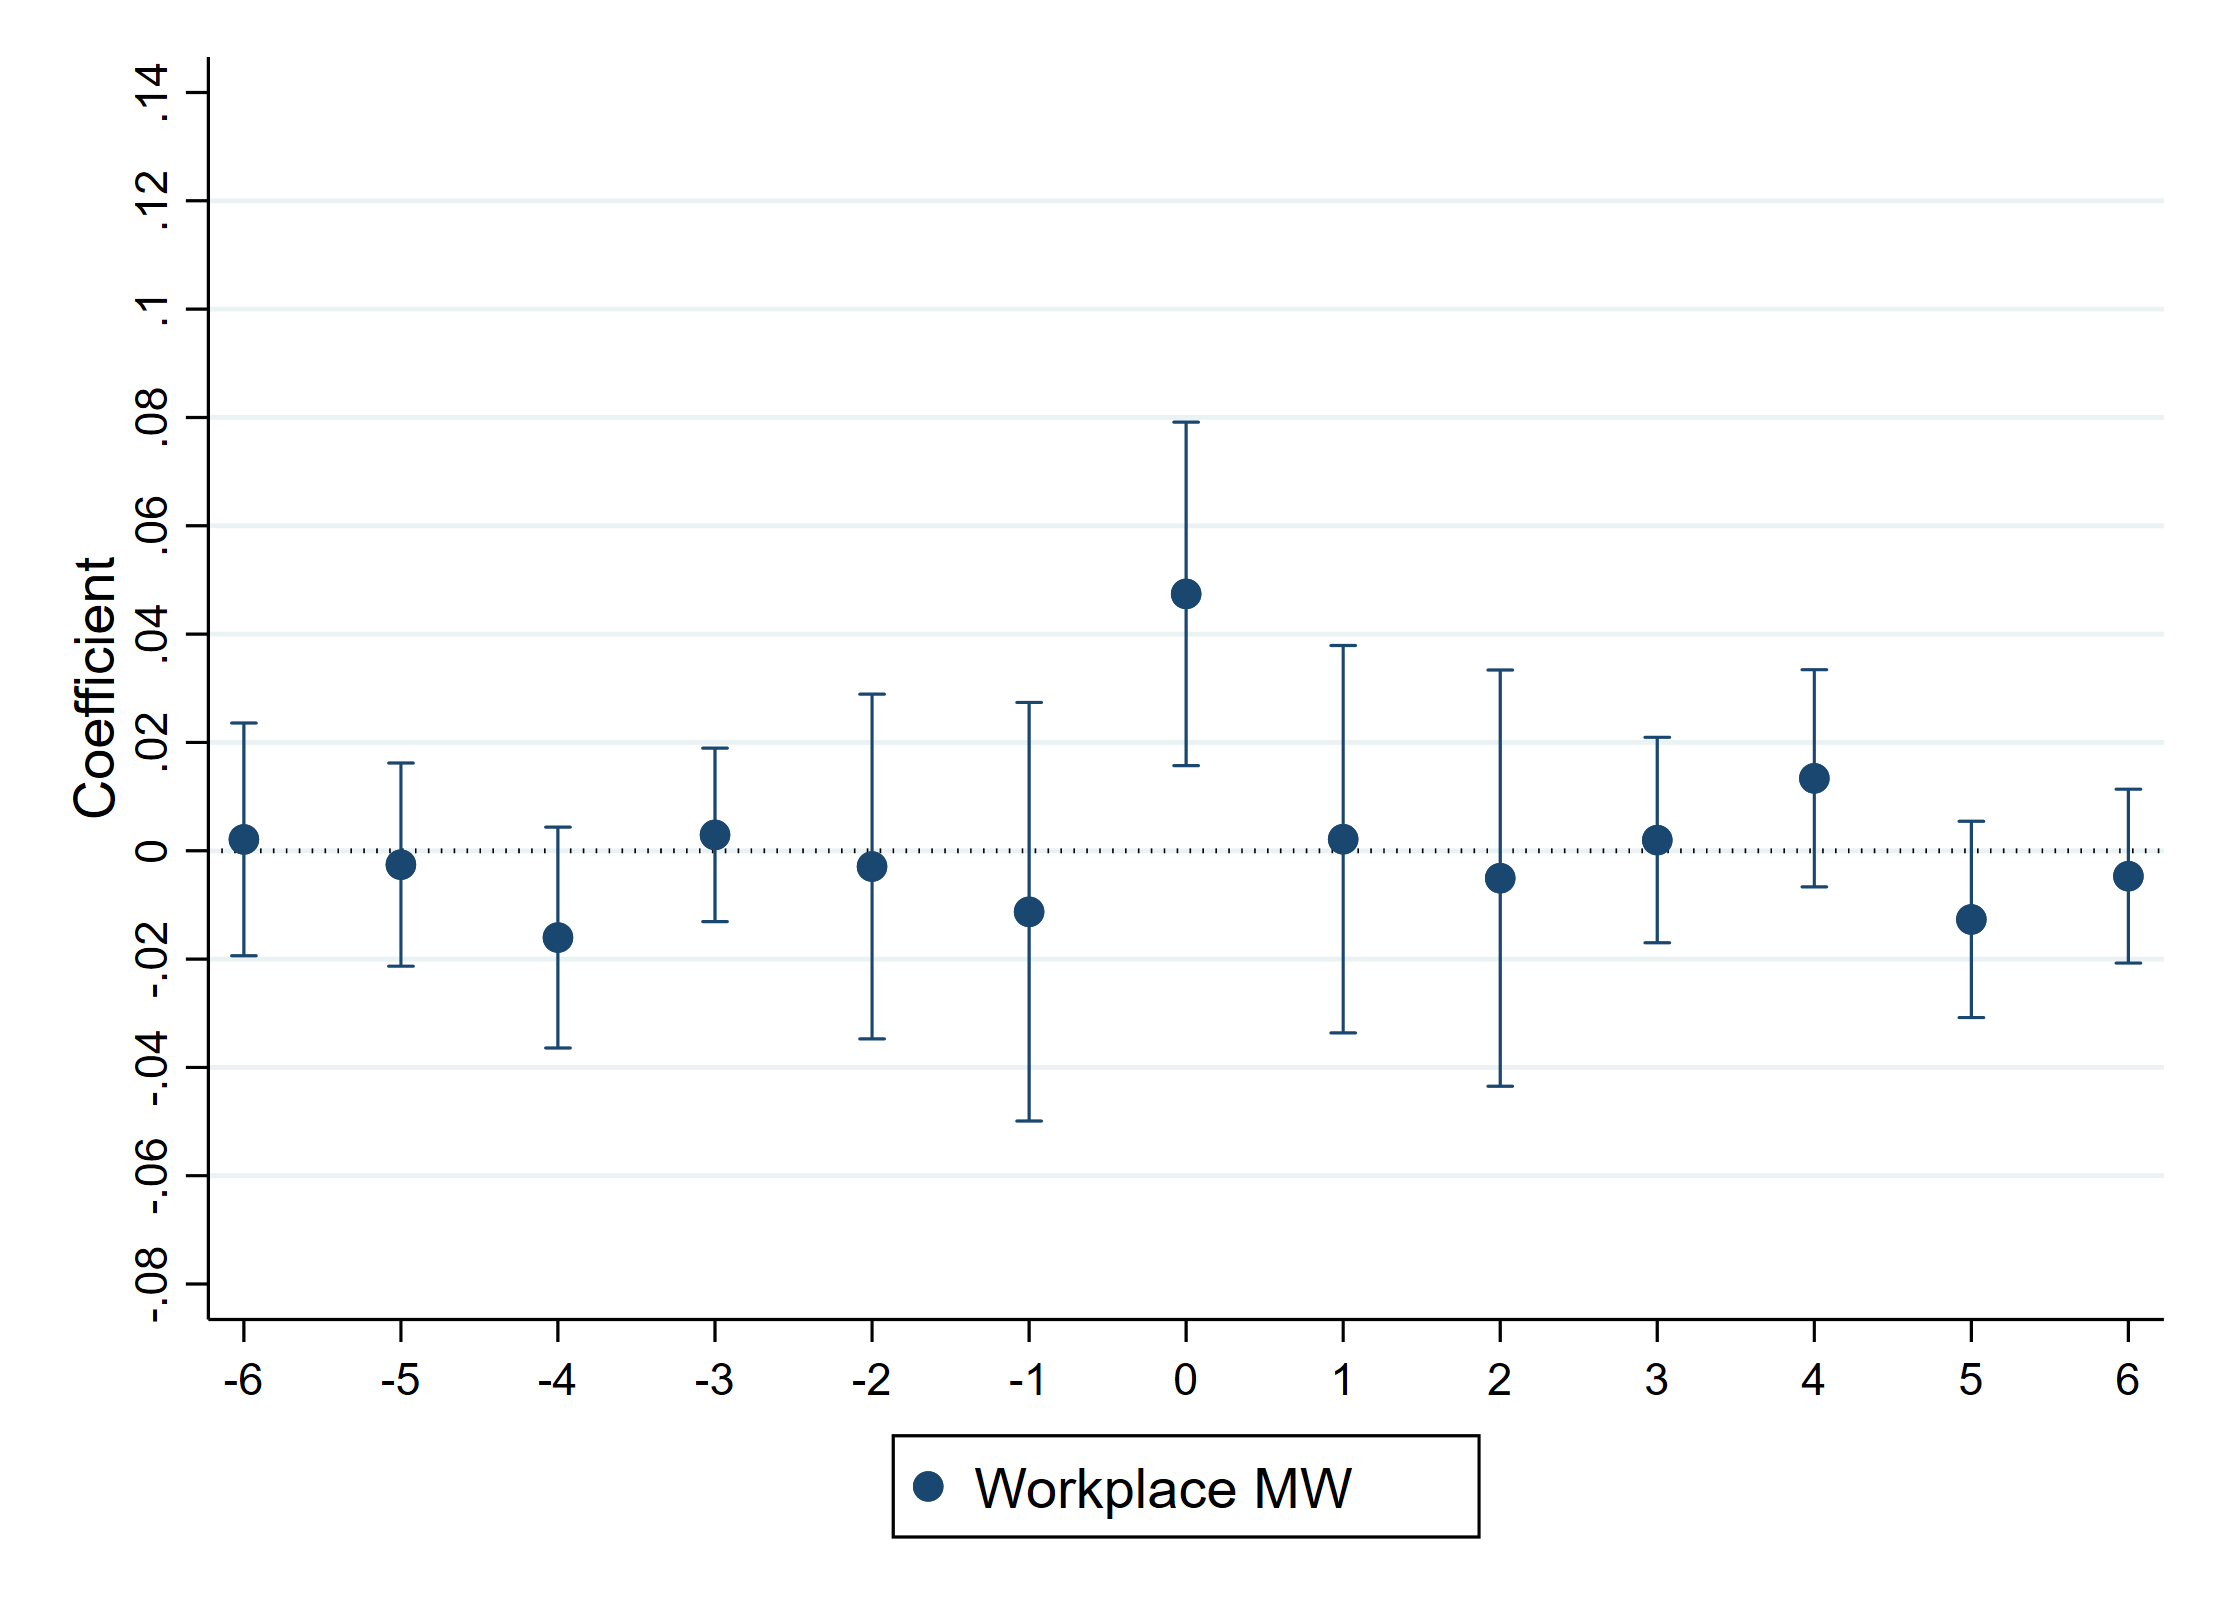
\includegraphics[width=0.68\textwidth]{fd_baseline/output/fd_mw_wkp_only_dynamic.png}
    \end{figure}
    
    \hyperlink{dyn_baseline_plot}{\beamerbutton{Go Back}}
\end{frame}

\begin{frame}[label = res_only_dyn]
    \frametitle{Including leads and lags of residence MW}

    \begin{figure}
        \centering
        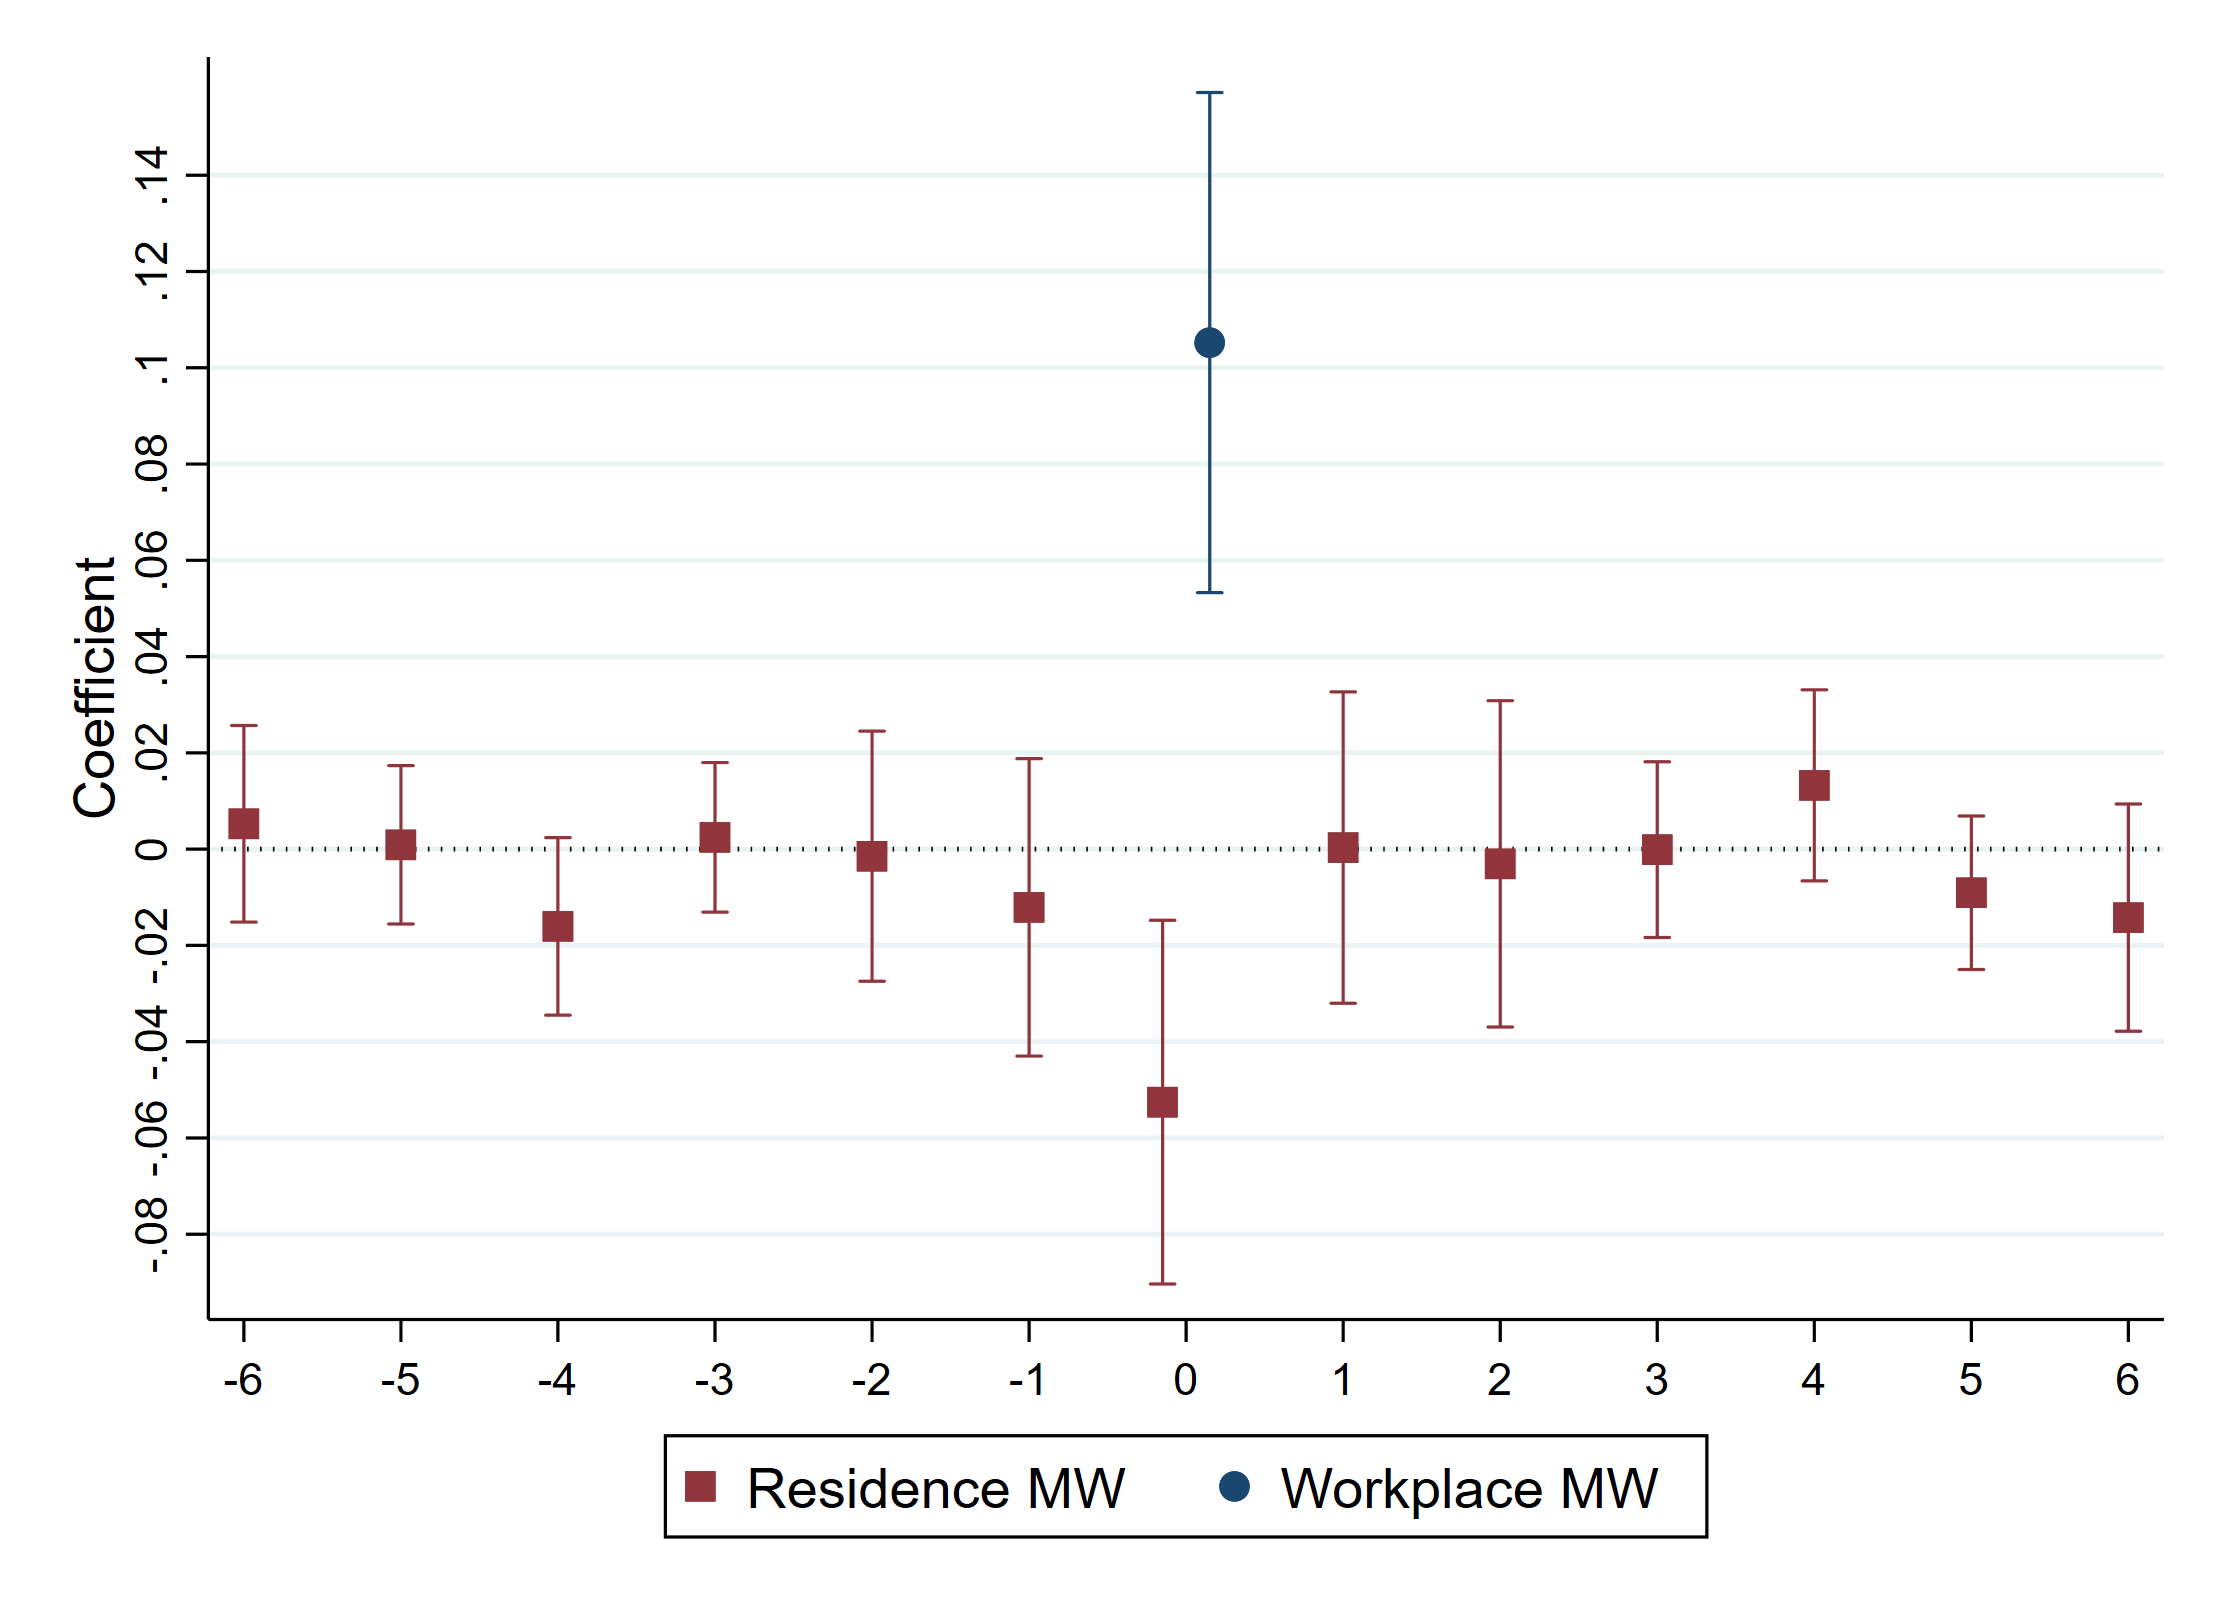
\includegraphics[width=0.68\textwidth]{fd_baseline/output/fd_both_mw_res_only_dynamic.png}
    \end{figure}
    
    \hyperlink{dyn_baseline_plot}{\beamerbutton{Go Back}}
\end{frame}

\begin{frame}[label = both_dyn]
    \frametitle{Including leads and lags of both MW measures}

    \begin{figure}
        \centering
        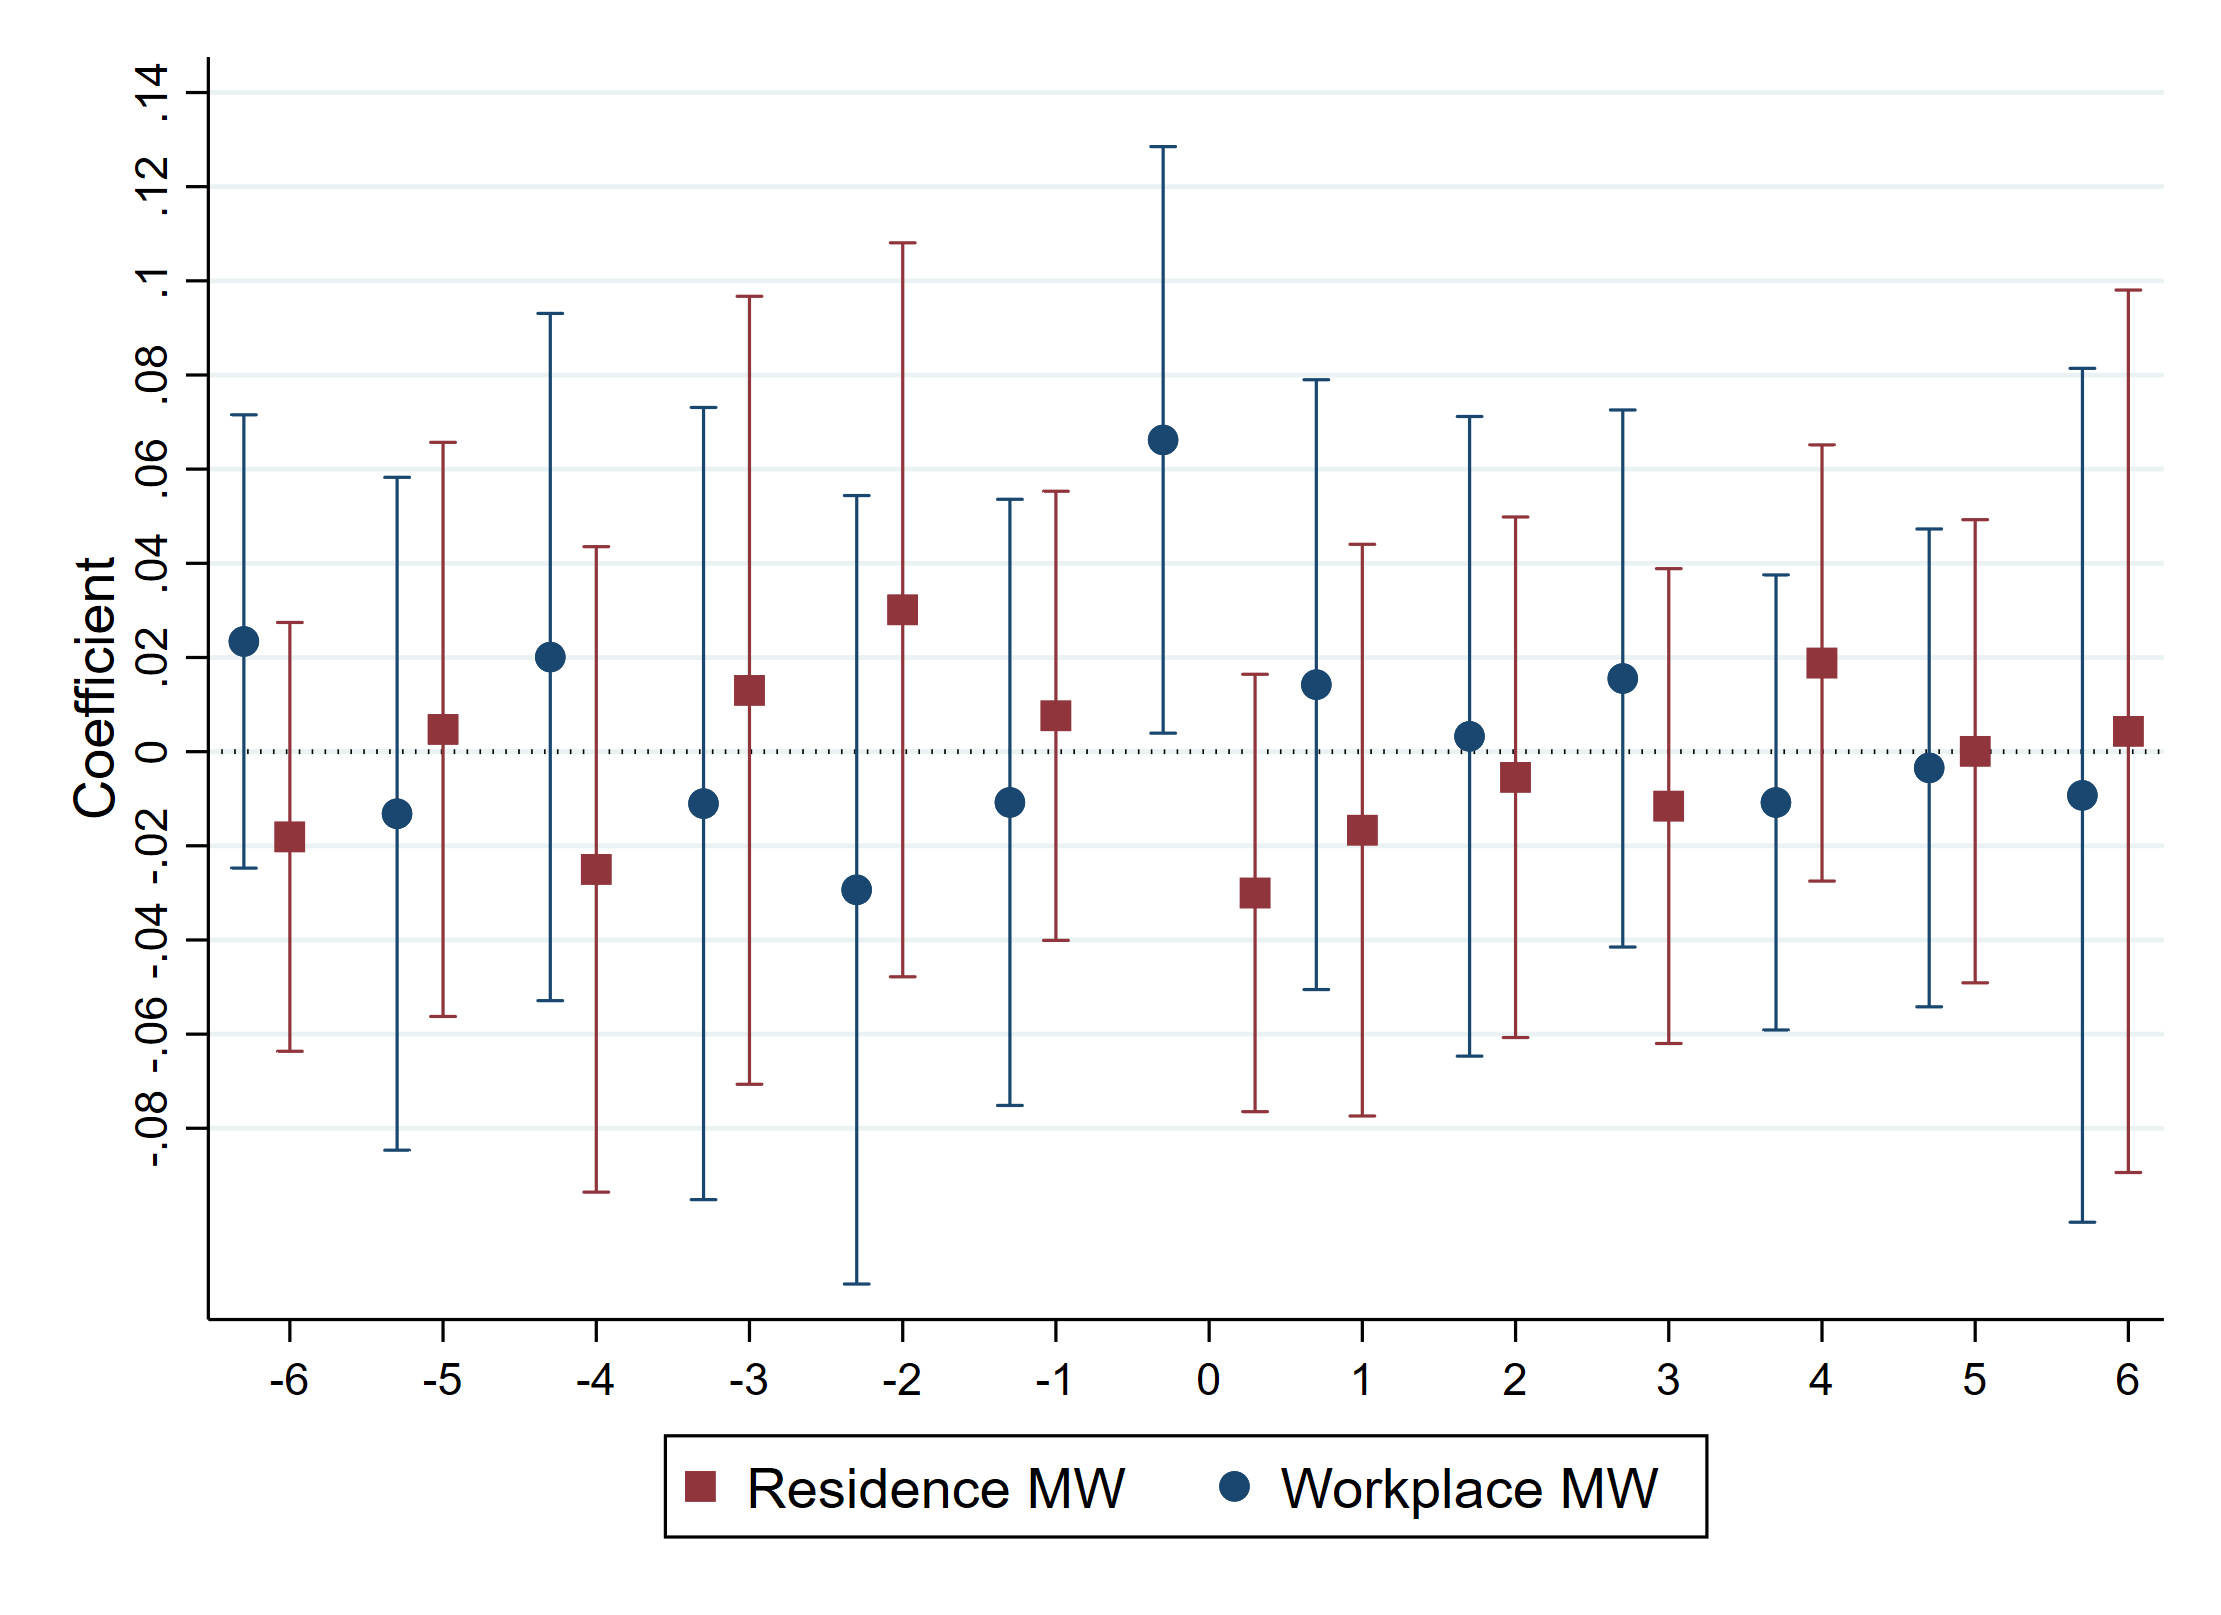
\includegraphics[width=0.68\textwidth]{fd_baseline/output/fd_both_dynamic.png}
    \end{figure}
    
    \hyperlink{dyn_baseline_plot}{\beamerbutton{Go Back}}
\end{frame}

\begin{frame}[label = robustness_sample]
    \frametitle{Sample selection concerns}

    \begin{table}
    \label{tab:static_sample}
    \scalebox{0.65}{
    \begin{tabular}{@{}lcccccc@{}}
        \toprule
                                           & \multicolumn{6}{c}{Change log rents}                                     \\ \cmidrule(l){2-7} 
                                           & \shortstack{Baseline\\(1)}       & \shortstack{Baseline\\Reweighted (2)}
                                           & \shortstack{Unbalanced\\(3)}     & \shortstack{Unbalanced\\Reweighted (4)}
                                           & \shortstack{Fully-balanced\\(5)} & \shortstack{Fully-balanced\\Reweighted (6)}  \\ \midrule
        Change residence minimum wage      & -0.0204      & -0.0077        & -0.0240       & -0.0163      & -0.0194     & 0.0032            \\
                                           & (0.0169)    & (0.0177)      & (0.0200)     & (0.0192)    & (0.0198)   & (0.0158)          \\
        Change workplace minimum wage      & 0.0545      & 0.0466        & 0.0461       & 0.0376      & 0.0678     & 0.0493            \\
                                           & (0.0283)    & (0.0303)      & (0.0305)     & (0.0343)    & (0.0308)   & (0.0293)          \\ \midrule
        P-value equality                   & 0.0965      & 0.2500        & 0.1586       & 0.3048      & 0.0826     & 0.2983            \\
        R-squared                          & 0.0209      & 0.0205        & 0.0160       & 0.0146      & 0.0216     & 0.0205            \\
        Observations                       & 131,383     & 125,502       & 193,292      & 185,198     & 78,912    & 75,447           \\ \bottomrule
    \end{tabular}
    }
\end{table}

    
    \hyperlink{robustness}{\beamerbutton{Go back}}
\end{frame}

\begin{frame}[label = wages_results]
    \frametitle{Estimates of the effect of the MW on total wages in a ZIP code}

    \vspace{2mm}
    \begin{table}[hbt!]
    \centering
    \label{tab:static_wages}

    \scalebox{0.87}{
    \begin{tabular}{@{}lccccc@{}}
        \toprule
                                & \multicolumn{4}{c}{Log total wages}
                                & \multicolumn{1}{c}{Log dividends}                        \\ \cmidrule(lr){2-5}\cmidrule(lr){6-6}
                                & (1)       & (2)      & (3)      & (4)       & (5)        \\ \midrule
        Workplace MW            & 0.1275       & 0.0909      & 0.1013      & 0.1013       & 0.0169        \\
                                & (0.0522)     & (0.0336)    & (0.0274)    & (0.0272)     & (0.0653)      \\ \midrule
        Sample                  & All       & All      & All      & Baseline  & All        \\
        Economic controls       & No        & Yes      & Yes      & Yes       & Yes        \\
        CBSA $\times$ year FE   & No        & No       & Yes      & Yes       & Yes        \\
        Within R-squared        & 0.0216       & 0.0090      & 0.0158      & 0.0953       & 0.0165        \\
        Observations            & 0      & 0     & 163,417     & 146,824      & 146,759       \\ \bottomrule
    \end{tabular}
    }
\end{table}


    
    \vspace{2mm}
    {\footnotesize
    Notes: unit of observation is ZIP code by year pairs. 
    All regressions include ZIP code FE and year FE.
    Workplace MW measure is yearly average of monthly 2017 variable.}

    \vspace{2mm}
    \hyperlink{share_pocketed_model}{\beamerbutton{Go back}}
\end{frame}

\end{document}